%%%%%%%%%%%%%%%%%%%%%%%%%%%%%%%%%%%%%%%%%%%%%%%%%%%%%%%%%%%%%%%%%%%%%%%%%%%%%%%%%%%%%%%%%%%%%%%%%%%%%
%% \section{Collaborators}

%% \begin{frame}
%%   \frametitle{Collaborators}
%%   \begin{itemize}
%%   \item Prof. Trygve Helgaker
%%   \item Dr. Simen Reine
%%   \item Dr. Thomas Bondo Pedersen
%%   \item Dr. Thomas Kj{\ae}rgaard
%%   \end{itemize}
%% \end{frame}




%% %%%%%%%%%%%%%%%%%%%%%%%%%%%%%%%%%%%%%%%%%%%%%%%%%%%%%%%%%%%%%%%%%%%%%%%%%%%%%%%%%%%%%%%%%%%%%%%%%%%%%
%% %%%%% slide 1 
%% \begin{frame}{Outline}
%%   \footnotesize

%%   \begin{itemize}
%%   \item The Resolution-of-the-Identity (RI) approximation
%%   \item Methods exploiting locality to reach linear-scaling RI
%%   \item The PARI approximation
%%   \item Results and Analysis of convergence issues
%%   \item Conclusion
%%   \end{itemize}

%% \end{frame}

%%%%%%%%%%%%%%%%%%%%%%%%%%%%%%%%%%%%%%%%%%%%%%%%%%%%%%%%%%%%%%%%%%%%%%%%%%%%%%%%%%%%%%%%%%%%%%%%%%%%%
%%%%% 
\frametitle{Introduction}
\framesubtitle{Limitations of pure KS-DFT for large molecules}

\begin{frame}{Limitations of pure KS-DFT for large molecules}
  %\footnotesize
  \textbf{Large/Protein-like molecules:}
  \begin{itemize}
  \item self-interaction error increases with system size 
    \\ > {\red error on properties increases with system size} 
  \item vanishing HUMO-LUMO gap \\ > {\red fail to converge} (e.g. Insulin)
  \item Required starting-points: HF or Hybrid-DFT \\> {\red Bottleneck: exact exchange contribution!}
  \end{itemize}


  \textbf{How to construct the Fock/KS matrix efficiently?}
% \\ > possibly using fitting approximations!  
  %% \begin{itemize}
  %% \item {\blue Resolution-of-the-identity approach (RI)}:\\ by fitting the products of atomic orbitals $|\mu\nu) = \widetilde{ |\mu\nu) }$
  %% \end{itemize}
  
  
\end{frame}

%%%%%%%%%%%%%%%%%%%%%%%%%%%%%%%%%%%%%%%%%%%%%%%%%%%%%%%%%%%%%%%%%%%%%%%%%%%%%%%%%%%%%%%%%%%%%%%%%%%%%
\frametitle{The RI approximation}
\framesubtitle{}

\begin{frame}{The RI approximation}
  \footnotesize
  \begin{itemize}
  \item  Four-center two-electron integrals in AO basis (Mulliken notation)
    \beq
 \int_{{\mathbb R}^3} \int_{{\mathbb R}^3} \psi_a(\mathbf{r}_1)\psi_b(\mathbf{r}_1) \frac{1}{r_{12}} \psi_c(\mathbf{r}_2)\psi_d(\mathbf{r}_2)
    d\mathbf{r}_1d\mathbf{r}_2 =    (ab|cd)
    \eeq

  \item Approximate AO-product functions:  $ {\blue |cd)} \approx  {\blue | \widetilde{cd})} = {\blue \sum_{\gamma} C_{\gamma}^{cd}|\gamma) } $

  \item Robust integral approximation (Dunlap)
    \beq
    (ab|cd) \approx (\widetilde{ab|cd}) = (\widetilde{ab}|cd) + (ab|\widetilde{cd}) - (\widetilde{ab}|\widetilde{cd})
    \eeq

  \item Error on integrals bounded with {\blue $\Delta_{ab} = |cd) - |\widetilde{cd} ) $ }
    \beq
    \vert (ab|cd) - (\widetilde{ab|cd}) \vert  \leq \sqrt{ (\Delta_{ab} | \Delta_{ab}) (\Delta_{cd} | \Delta_{cd}) }
    \eeq

  \item Find fitting coefficients $ {\blue C_{\alpha}^{ab} }$  for each AO-product $|ab)$
    \beq
    \min_{\mathbf{C}} (\Delta_{ab} \vert \Delta_{ab}) \Longleftrightarrow (\Delta_{ab} \vert \alpha) = 0  \ \ \ \forall \alpha
    \eeq

  \end{itemize}
\end{frame}



%%%%%%%%%%%%%%%%%%%%%%%%%%%%%%%%%%%%%%%%%%%%%%%%%%%%%%%%%%%%%%%%%%%%%%%%%%%%%%%%%%%%%%%%%%%%%%%%%%%%%
%%%%% slide 2
\frametitle{The RI approximation: Pros \& Limitations}
\framesubtitle{}

\begin{frame}{The RI approximation}
  \footnotesize

  The {\blue Resolution-of-the-Identity (RI)}, or the {\blue density-fitting (DF)} approximation:
  \begin{itemize}
  \item Speed up calculations ({\blue typically by factor 3-30}) at little loss of chemical accuracy
  \item Highly successful for {\blue approximating the Coulomb contribution} (in particular in DFT)
  \item Also used for small- to medium-sized systems for {\blue approximation of the exact exchange} and 
    in correlated treatment \\ > {\red Scaling wall} about 1000 AO basis-functions
%  \item  The {\red  auxiliary basis set} defines the smallest error on integrals
  \end{itemize}
\end{frame}

%%%%%%%%%%%%%%%%%%%%%%%%%%%%%%%%%%%%%%%%%%%%%%%%%%%%%%%%%%%%%%%%%%%%%%%%%%%%%%%%%%%%%%%%%%%%%%%%%%%%%
%%%%% slide 4
\frametitle{}
\framesubtitle{}

\begin{frame}{RI for the exact exchange (RI-K)}
  \footnotesize
  \begin{itemize}
  \item The (regular) exchange contribution
    \begin{eec}
      K_{ab} = \sum_{ab} (ac|bd) D_{cd} = \sum_i^\text{occ} (a i | b i) 
    \end{eec}
    %% \begin{eec}
    %%   \tilde K_{\mu\nu} = \sum_{\gamma\delta} \sum_{IJ} (\mu\gamma|I)(I|J)^{-1}(J|\nu\delta) D_{\gamma\delta}
    %%   = \sum_i^\text{occ} \sum_{IJ} (\mu i |I)(I|J)^{-1}(J| \nu i)
    %% \end{eec}
    {\tiny {\blue Weigend (2002), Polly~\emph{et.al} (2004)} }

  \item in RI-K, each pair is fitted over the whole molecule \\{\red Too expensive, not even needed: ``contaminants''!}
    \\the {\red Scaling wall} limits the approach to about 1000 AO basis-functions

    \begin{itemize}
      \footnotesize
    \item metric matrix $\blue (I|J)$ non-sparse $\red \to {\cal O}(N^3)$ scaling
    \item non-locality of fitting coefficients $\blue c_I^{\mu\nu}$ (\red for each pair $\mu\nu$)
    \end{itemize}
  \item  Exchange and Correlation are local phenomena
\\    {\red Locality has to be exploited!}
  \end{itemize}
\end{frame}

%%%%%%%%%%%%%%%%%%%%%%%%%%%%%%%%%%%%%%%%%%%%%%%%%%%%%%%%%%%%%%%%%%%%%%%%%%%%%%%%%%%%%%%%%%%%%%%%%%%%%
%%%%% slide 5.1
\frametitle{}
\framesubtitle{}

\begin{frame}{Methods for linear-scaling RI}
  \footnotesize

  Two main approaches forcing locality toward linear-scaling RI:
  \begin{itemize}
  \item {\red the Local Metric approach}
    \\Obtain the fitting coefficients using (\textit{w}) a local metric
    \\(e.g. the overlap metric)
    \\{\tiny {\blue Baerends~\emph{et.al} (1973), Vahtras~\emph{et.al} (1993), Jung~\emph{et.al} (2005), Reine~\emph{et.al} (2008)} }
    %% \begin{eec}
    %%   c_I^{\mu\nu} = \sum_J \langle I|w|J \rangle^{-1} \langle J|w|\mu\nu\rangle
    %% \end{eec}
    %% instead of the Coulomb metric
    %% \begin{eec}
    %%   \blue c_I^{\mu\nu} = \sum_J (I|J)^{-1} (J|\mu\nu)
    %% \end{eec}
  \item {\red the Partitioning approach}
    \\Partition the density and fit each density in a local region 
    \\{\tiny {\blue Gallant and St-Amant (1996), Sodt~\emph{et.al} (2006), Sodt and Head-Gordon (2008)} }
    %\begin{eec}
    %  \rho(\mathbf{r}) = \sum_s \rho^s(\mathbf{r}), \quad \red \rho^s(\mathbf{r}) \approx \tilde\rho^s(\mathbf{r})
    %\end{eec}
    \begin{itemize}
  \footnotesize
      \item e.g. The Atomic RI (ARI)
    \end{itemize}
  \end{itemize}
\end{frame}

%%%%%%%%%%%%%%%%%%%%%%%%%%%%%%%%%%%%%%%%%%%%%%%%%%%%%%%%%%%%%%%%%%%%%%%%%%%%%%%%%%%%%%%%%%%%%%%%%%%%%
%%%%% slide 5.2
\frametitle{}
\framesubtitle{}

\begin{frame}{Methods for linear-scaling RI}
  \footnotesize
  %
      {\blue Atomic RI (ARI)}: an elegant and balanced partitioning approach:
      \begin{itemize}
      \item In the ARI approach of Sodt~\emph{et.al} each charge distribution $\blue |\mu\nu)$ is 
        first associated with a center $\blue C$, and is fitted using auxiliary functions 
        $\blue |I)$ centered on the atoms in some buffer zone $\blue [C]$ around $\blue C$ 

        \begin{eec}
          |\mu\nu) = \sum_I c_I^{\mu\nu} |I), \quad \red |I) \in [C]
        \end{eec}
        \begin{itemize}
          \footnotesize 
        \item fixed buffer-zone size - {\red system dependent}
        \item the set $\blue |I)$ includes the {\red auxiliary functions centered on several atoms}
        \end{itemize}
      %% \item Jung~\emph{et.al} explored the decay behavior of the two-center fitting coefficients
      %%   $\blue c_I^{\mu\nu}$. 
      %%   \begin{itemize}
      %%     \footnotesize 
      %%   \item Coulomb metric fit - the asymptotic decay of $\blue c_I^{\mu\nu}$ was as slow 
      %%     as $\red \frac{1}{r}$
      %%   \item local ({\blue overlap/attenuated Coulomb}) metric fit - {\red exponential decay} with distance
      %%   \item But the fitting errors $\approx 10$ times smaller in the Coulomb than in the overlap metric
      %%   \end{itemize}
      \end{itemize}

\end{frame}


%%%%%%%%%%%%%%%%%%%%%%%%%%%%%%%%%%%%%%%%%%%%%%%%%%%%%%%%%%%%%%%%%%%%%%%%%%%%%%%%%%%%%%%%%%%%%%%%%%%%%
%%%%% slide 6.1
\frametitle{}
\framesubtitle{}

\begin{frame}{The PARI approach}
  \footnotesize

  We propose the pair-atomic resolution-of-the-identity (PARI):
  \begin{itemize}
  \item fit each charge distribution $\blue |\mu\nu)$ with auxiliary functions
    $\blue |I)$ centered on the two parent atoms $\blue A$ and $\blue B$ of 
    the basis functions $\blue |\mu)$ and $\blue |\nu)$
    \begin{eec}
      |\widetilde{\mu\nu}) = \sum_{I\in{A\cup B}} c_I^{\mu\nu}|I), 
      \quad c_I^{\mu\nu} = \sum_{\red J\in{A\cup B}} (I|J)^{-1}(J|\mu\nu)
    \end{eec}
    instead of the (regular) RI approx.
    \begin{eec}
      |\widetilde{\mu\nu}) = \sum_{I\in{\cal M}} c_I^{\mu\nu}|I), 
      \quad c_I^{\mu\nu} = \sum_{\red J\in{\cal M}} (I|J)^{-1}(J|\mu\nu)
    \end{eec}
  %% \item replace all $\blue (\mu\nu|\gamma\delta)$ by {\red robust} and {\red variational} 
  %%   $\blue \widetilde{(\mu\nu|\gamma\delta)}$ given by
  %%   \begin{equation*}
  %%     \begin{split}
  %%       \blue
  %%       \widetilde{(\mu\nu|\gamma\delta)} &\blue= (\mu\nu|\widetilde{\gamma\delta}) 
  %%       + (\widetilde{\mu\nu}|\gamma\delta) - (\widetilde{\mu\nu}|\widetilde{\gamma\delta})\\
  %%       & = \blue (\mu\nu|\gamma\delta) - \red (\mu\nu-\widetilde{\mu\nu}|\gamma\delta-\widetilde{\gamma\delta})
  %%     \end{split}
  %%   \end{equation*}
  \item Pros/Cons:
    \begin{itemize}
  \footnotesize
    \item Highly local : \textbf{ {\blue removes scaling bottleneck } }
    \item Straightforwardly linear scaling using screening and FMM
    \item {\red decreases accuracy} $\to$ larger auxiliary basis sets
    \item \textbf{ {\red some unpredictable $\&$ spectacular diverging cases!!!} }
    \end{itemize}
  \end{itemize}

\end{frame}
%
%% %%%%%%%%%%%%%%%%%%%%%%%%%%%%%%%%%%%%%%%%%%%%%%%%%%%%%%%%%%%%%%%%%%%%%%%%%%%%%%%%%%%%%%%%%%%%%%%%%%%%%
%% %%%%% slide 6.2
%% \frametitle{}
%% \framesubtitle{}

%% \begin{frame}{PARI-J}
%%   \footnotesize

%%   PARI for the Coulomb contribution (PARI-J)
%%   \begin{equation*}
%%     \begin{split}
%%       \widetilde{J}_{\mu\nu} &=  \sum_{\gamma\delta} \widetilde{(\mu\nu|\gamma\delta)} D_{\gamma\delta} 
%%       = \sum_{\gamma\delta} \left[  (\widetilde{\mu\nu}|\gamma\delta) +  (\mu\nu|\widetilde{\gamma\delta}) -  (\widetilde{\mu\nu}|\widetilde{\gamma\delta}) \right]  D_{\gamma\delta}\\
%%       &=  \sum_{\gamma\delta} \left[ \sum_{I\in{A\cup B}}c_I^{\mu\nu} (I|\gamma\delta) + \sum_{J\in{C\cup D}} (\mu\nu|J) c_J^{\gamma\delta} - \sum_{I\in{A\cup B},J\in{C\cup D}}c_I^{\mu\nu} (I|J) c_J^{\gamma\delta} \right]  D_{\gamma\delta}\\
%%       &=  \sum_{I\in{A\cup B}}c_I^{\mu\nu} (I|\rho) + \sum_{J\in{C\cup D}} (\mu\nu|J) c_J - \sum_{I\in{A\cup B}}c_I^{\mu\nu} (I| \tilde{\rho}),  with \quad \red c_J = \sum_{\gamma\delta} c_J^{\gamma\delta} D_{\gamma\delta} \\
%%       &= \sum_{J\in{C\cup D}} (\mu\nu|J) c_J +  \sum_{I\in{A\cup B}}c_I^{\mu\nu} (I|\rho-\tilde{\rho}), with \quad 
%%       \blue |\tilde\rho) = \sum_J c_J|J),  \red \sum_J (I|J)c_J = (J|\rho) \\
%%       & = \sum_I (\mu\nu|I)c_I + \sum_{I\in{A\cup B}} C_I^{\mu\nu}(I|\rho-\tilde\rho)
%%     \end{split}
%%   \end{equation*}
%%   \begin{itemize}
%%   \item straightforwardly linear scaling using screening and FMM
%%   \end{itemize}
%% \end{frame}
%% %

%% %%%%%%%%%%%%%%%%%%%%%%%%%%%%%%%%%%%%%%%%%%%%%%%%%%%%%%%%%%%%%%%%%%%%%%%%%%%%%%%%%%%%%%%%%%%%%%%%%%%%
%% %%%%% slide 6.3
%% \frametitle{}
%% \framesubtitle{}

%% \begin{frame}{PARI-K}
%%   \footnotesize

%%   PARI for the Exact-Exchange contribution (PARI-K)
%%   \begin{itemize}
%%   \item split fitting coefficients into the two parent atoms
%%     \begin{eec}
%%       |\widetilde{\mu\nu}) = 
%%       |\widetilde{\underbar{$\mu$}\nu}) + |\widetilde{\mu\underbar{$\nu$}}), 
%%       \quad \red |\widetilde{\underbar{$\mu$}\nu}) = \sum_{I\in A} c_I^{\mu\nu} |I),
%%       \quad \blue |\mu\widetilde{\underbar{$\nu$}}) = \sum_{J\in B} c_J^{\mu\nu} |J)
%%     \end{eec}
%%   \item leads to a splitting of $\blue \widetilde{(\mu\nu|\gamma\delta)}$ into eight parts
%%     - four involving three-center and four two-center integrals
%%   \item collect terms in order to calculate each integral only once and select 
%%     contraction pathway in order to reduce cost
%%   \item exploit symmetry of integrals and density matrix 
%%   \end{itemize}
%%   An example three-center term:
%%   \begin{equation*}
%%     \blue K_{\mu\gamma} \stackrel{+}{=} \sum\limits_{I\delta} d_{I,\delta}^\mu (I|\gamma\delta), 
%%     \quad \red I,\mu\in A,\blue \gamma\in C, \red \delta\in {\cal M}, \quad
%%     \blue d_{I,\gamma}^\mu = \sum\limits_\nu c_I^{\mu\nu}D_{\nu\gamma}
%%     %\begin{split}
%%     % \blue K_{\mu\gamma} &\blue\stackrel{+}{=} \sum\limits_{I\delta} d_{I,\delta}^\mu (I|\gamma\delta), \quad \red I,\mu\in A,\blue \gamma\in C, \red \delta\in {\cal M}\\
%%     % \blue d_{I,\gamma}^\mu &\blue = \sum\limits_\nu c_I^{\mu\nu}D_{\nu\gamma}
%%     %\end{split}
%%   \end{equation*}
%%   \begin{itemize}
%%   \item ignoring screening each of these terms scale $\blue {\cal O}(N^3 n^3 a)$\\
%%     number of atoms $\blue N$, of regular/auxiliary basis functions per atom 
%%     $\blue n$,$\blue a$
%%   \item to be compared with the $\red {\cal O}(N^4 n^2 a^2)$ scaling of conventional RI
%%     %- {\blue can be reduced to $\red {\cal O}(N^3 N_\text{occ} n a^2)$ using MOs, with $\red N_\text{occ}$ the number of occupied MOs}
%%   \end{itemize}
%% \end{frame}
%% %
%% %%%%%%%%%%%%%%%%%%%%%%%%%%%%%%%%%%%%%%%%%%%%%%%%%%%%%%%%%%%%%%%%%%%%%%%%%%%%%%%%%%%%%%%%%%%%%%%%%%%%%
%% %%%%% slide 7
%% \frametitle{}
%% \framesubtitle{}

%% \begin{frame}{ Outline of PARI-K algorithm}
%%   \footnotesize
%%   \begin{figure}
%%     \begin{tabbing}
%%       \hspace{3pt}\=\hspace{10pt}\=\hspace{10pt}\=\hspace{10pt}\=\hspace{10pt}\=\hspace{10pt}\=\hspace{10pt}\=\hspace{10pt}\=\hspace{10pt}\=\hspace{10pt}\kill
%%       \> {\blue Three-center contributions} \\
%%       \> Loop $A$ \\
%%       \> \> Calculate the fitting coefficients $\blue c_I^{\mu\nu}, \quad \red I,\mu\in A, \blue \nu\in {\cal M}$ \\
%%       \> \> and density coefficients $\blue d_{I,\gamma}^\mu $ \\
%%       %\> \> Construct density coefficients $\blue d_{I,\gamma}^\mu $\\
%%       \> \> Loop $C$ \\
%%       \> \> \> Loop $D\ge C$ \\
%%       \> \> \> \> Calculate $\blue (I|\gamma\delta), \quad \red I\in A,\blue\gamma\in C, \red\delta\in D$ \\
%%       \> \> \> \> Make contractions \\
%%       \> \> \> \> \> $\blue \tilde K_{\mu\gamma} \stackrel{+}{=} \sum\limits_{I\delta} d_{I,\delta}^\mu (I|\gamma\delta), \red \quad {\cal O}(N^3 n^3 a)$ \\
%%       \> \> \> \> \> $\blue \tilde K_{\mu\delta} \stackrel{+}{=} \sum\limits_{I\gamma} d_{I,\gamma}^\mu (I|\gamma\delta), \red \quad {\cal O}(N^3 n^3 a)$ \\
%%       \> \> \> \> \> $\blue X_{I,\gamma}^\mu = \sum\limits_\delta (I|\gamma\delta)D_{\mu\delta}, \red \quad {\cal O}(N^3 n^3 a)$ \\
%%       \> \> \> \> \> $\blue X_{I,\delta}^\mu = \sum\limits_\gamma (I|\gamma\delta)D_{\mu\gamma}, \red \quad {\cal O}(N^3 n^3 a)$ \\
%%       %\> \> \> End loop $D$ \\
%%       \> \> Make contractions \\
%%       \> \> \> $\blue \tilde K_{\nu \gamma} \stackrel{+}{=} \sum_{I,\mu} c_{I}^{\mu\nu} X_{I,\gamma}^\mu, \red \quad {\cal O}(N^3 n^3 a)$ \\
%%       \> \> \> $\blue \tilde K_{\nu \delta} \stackrel{+}{=} \sum_{I,\mu} c_{I}^{\mu\nu} X_{I,\delta}^\mu, \red \quad {\cal O}(N^3 n^3 a)$ \\
%%       %\> \> End loop $C$ \\
%%       %\> End loop $A$ \\
%%       \> Symmetrized or anti-symmetrized $\blue \mathbf{\tilde K}$ \\
%%     \end{tabbing}
%%   \end{figure}
%% \end{frame}


%%%%%%%%%%%%%%%%%%%%%%%%%%%%%%%%%%%%%%%%%%%%%%%%%%%%%%%%%%%%%%%%%%%%%%%%%%%%%%%%%%%%%%%%%%%%%%
%%%%% slide 8
\begin{frame}{PARI Accuracy}
  \footnotesize

\begin{center}
  G2/G3   Benchmark set (480 molecules),
  \\ B3LYP, 6-31G/df-def2, in $\mu E_H$
\\      {\tiny{Development version of LSDalton, www.daltonprogram.org}}
\begin{tabular}{lccccc}
\hline
\hline
&  &  RI-J  &  PARI-J  &  RI-K  &  PARI-K   \\ 
\cline{2-6}
\multirow{3}{*}{6-31G/df-def2}          & $\mu$    & -21 & -74 & 8  & 21 \\  
                                        & $\sigma$ & 9   & 48  & 3  & 10 \\  
\hline
\multirow{3}{*}{ cc-pVTZ/cc-pVTZdenfit}  & $\mu$   & -18 & -22 & 9  & 14 \\  
                                        & $\sigma$ & 4   & 11  & 3  & 7 \\  
\hline
\hline
\end{tabular}
\end{center}

  \begin{itemize}
  \item PARI errors: {\blue factor 2-3 bigger than RI  }
  \item {\red 4 molecules out of 480 with diverging negative energies!}
  \end{itemize}

\end{frame}


%% %%%%%%%%%%%%%%%%%%%%%%%%%%%%%%%%%%%%%%%%%%%%%%%%%%%%%%%%%%%%%%%%%%%%%%%%%%%%%%%%%%%%%%%%%%%%%%
%% %%%%% slide ...
%% \begin{frame}{Results and Analysis: Speed-up}
%%   \footnotesize

%% \begin{center}
%% 14 small to medium sized molecules
%%   \\ B3LYP, cc-pVTZ/cc-pVTZdenfit, in $\mu E_H$
%% \begin{tabular}{lc|c|c||c|c}  
%% \hline
%% \hline
%%    & J-engine   & PARI-J     & RI-J       & LinK       & RI-K     \\ 
%%    & timing (s) & speed-up  & speed-up  & timing (s) & speed-up  \\ 
%% \cline{2-6}
%% PA\_oligomer\_3 &  13 &   7 &  15 &  36 &   3 \\ 

%% benzene &  39 &   9 &  22 & 131 &   4 \\ 

%% PA\_oligomer\_4 &  40 &  10 &  21 & 113 &   3 \\ 

%% PA\_oligomer\_5 &  81 &  11 &  24 & 297 &   3 \\ 

%% dipeptide & 115 &  11 &  24 & 409 &   5 \\ 

%% acene\_1 & 171 &  15 &  31 & 478 &   4 \\ 

%% PA\_oligomer\_2 & 141 &  13 &  24 & 406 &   3 \\ 

%% beta-dipeptide & 169 &  13 &  26 & 625 &   4 \\ 

%% PP & 216 &  16 &  31 & 630 &   4 \\ 

%% dmabn & 235 &  16 &  31 & 826 &   5 \\ 

%% tripeptide & 267 &  14 &  29 & 964 &   3 \\ 

%% acene\_2 & 427 &  20 &  50 & 1319 &   5 \\ 

%% acene\_3 & 764 &  22 &  33 & 2385 &   4 \\ 

%% acene\_4 & 1249 &  26 &  39 & 3806 &   4 \\ 

%% acene\_5 & 1773 &  25 &  40 & 5477 &   4 \\ 

%% \hline
%% \hline
%% \end{tabular}
%% {\tiny{Development version of LSDalton, www.daltonprogram.org}}
%% \end{center}

%% \end{frame}



\section{Problem Analysis}
  \footnotesize
\begin{frame} 
   \frametitle{Problem Analysis:
     \\Attractive forces between the electrons....}
  \begin{itemize}
   \item Two-electron contribution to the total energy becomes negative ({\red attractive iteraction!})
   \item The robust integral representation, 
    \beq
    (ab|cd) \approx (\widetilde{ab|cd}) = (\widetilde{ab}|cd) + (ab|\widetilde{cd}) - (\widetilde{ab}|\widetilde{cd})
    \eeq
though accurate to second order in the fitting error
\\    {\red      not inherently positive-definite  ($(ab|ab)$ <0) sometimes 
\\NEGATIVE SHIFT OF THE EIGENVALUES }

   %% \item Positive semi-definite in:
   %%       \begin{itemize}
   %%          \item global fitting: always
   %%          \item local fitting: fitting basis locally complete
   %%       \end{itemize}
   \item The SCF solver does what it is supposed to: minimize the energy.
   \end{itemize}
\end{frame}







\begin{frame}
   \frametitle{Problem Analysis:
     \\ H$_2$ already infected by PARI}
  \footnotesize

  \begin{center}
    \begin{tabular}{crcccc}
      \hline
      \hline
      &            & exact    & RI    & PARI & PARI+diag(exact)  \\
      \cline{2-6}
      \multirow{3}{*}{H$_2$}        & mad(eri)    &  -     & 2.7   &   {\red 8.9 }      &  {\blue  0.36 }       \\
      \cline{2-6}
                                    & min(eigV)   & 4.4e-2 &1.5e-2 &  {\red-1.1  }     &   {\blue 5.85e-2}     \\
     \cline{2-6}
      & eigV$<0$    & 0/11   &  0/11 &  {\red 2} / 11      &  {\blue  0} / 11        \\
      \hline
      \hline
      \multirow{3}{*}{C$_2$H$_4$}   & mad(eri)    &  -     &  5.6  &    {\red  10.9 }   &  {\red  0.48 }        \\
      \cline{2-6}
      & min(eigV)   & 0      & 0     &    {\red -3.9  }  &   {\red -1.45}        \\
      \cline{2-6}
      & eigV$<0$    &  0/352 & 0/352 &    {\red 63} / 352  &    {\red  17} / 352     \\
      \hline
      \hline
    \end{tabular}
  \end{center}

PARI operator:
  \begin{itemize}
  \item  non-positive definite!!
  \item ``unbalanced'':
\\ $(ab|cd)$ with $a \in A$, $b \in B$ , $c \in C$ and $d \in D$ 
\\ $(ab|cd)$ with $a \in A$, $b \in A$ , $c \in B$ and $d \in B$ 
\\{\red not treated with the same basis set, not the same accuracy}
\\{\red UNBALANCED negative shift between the blocks $(AB|CD)$}

  \end{itemize}
\end{frame}




\section{One failing case ``cured'': but-3-yn-2-one}

\begin{frame}
   \frametitle{One failing case: but-3-yn-2-one}
    \begin{center}
        \begin{figure}
            \scalebox{0.6}{
                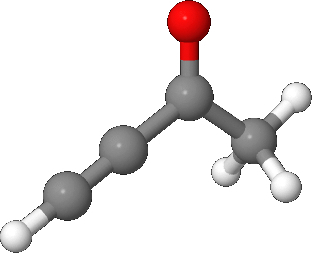
\includegraphics{Figures/c4h4o_transparent.jpg}
            }
        \end{figure}
    \end{center}
\end{frame}

\section{But-3-yn-2-one: SCF iterations, cc-pVTZdenfit}

\begin{frame}
   \frametitle{BLYP cc-pVTZ SCF iterations}
   \tiny{Development version of Molcas, www.molcas.org}
    \begin{center}
        \begin{figure}
            \scalebox{0.3}{
                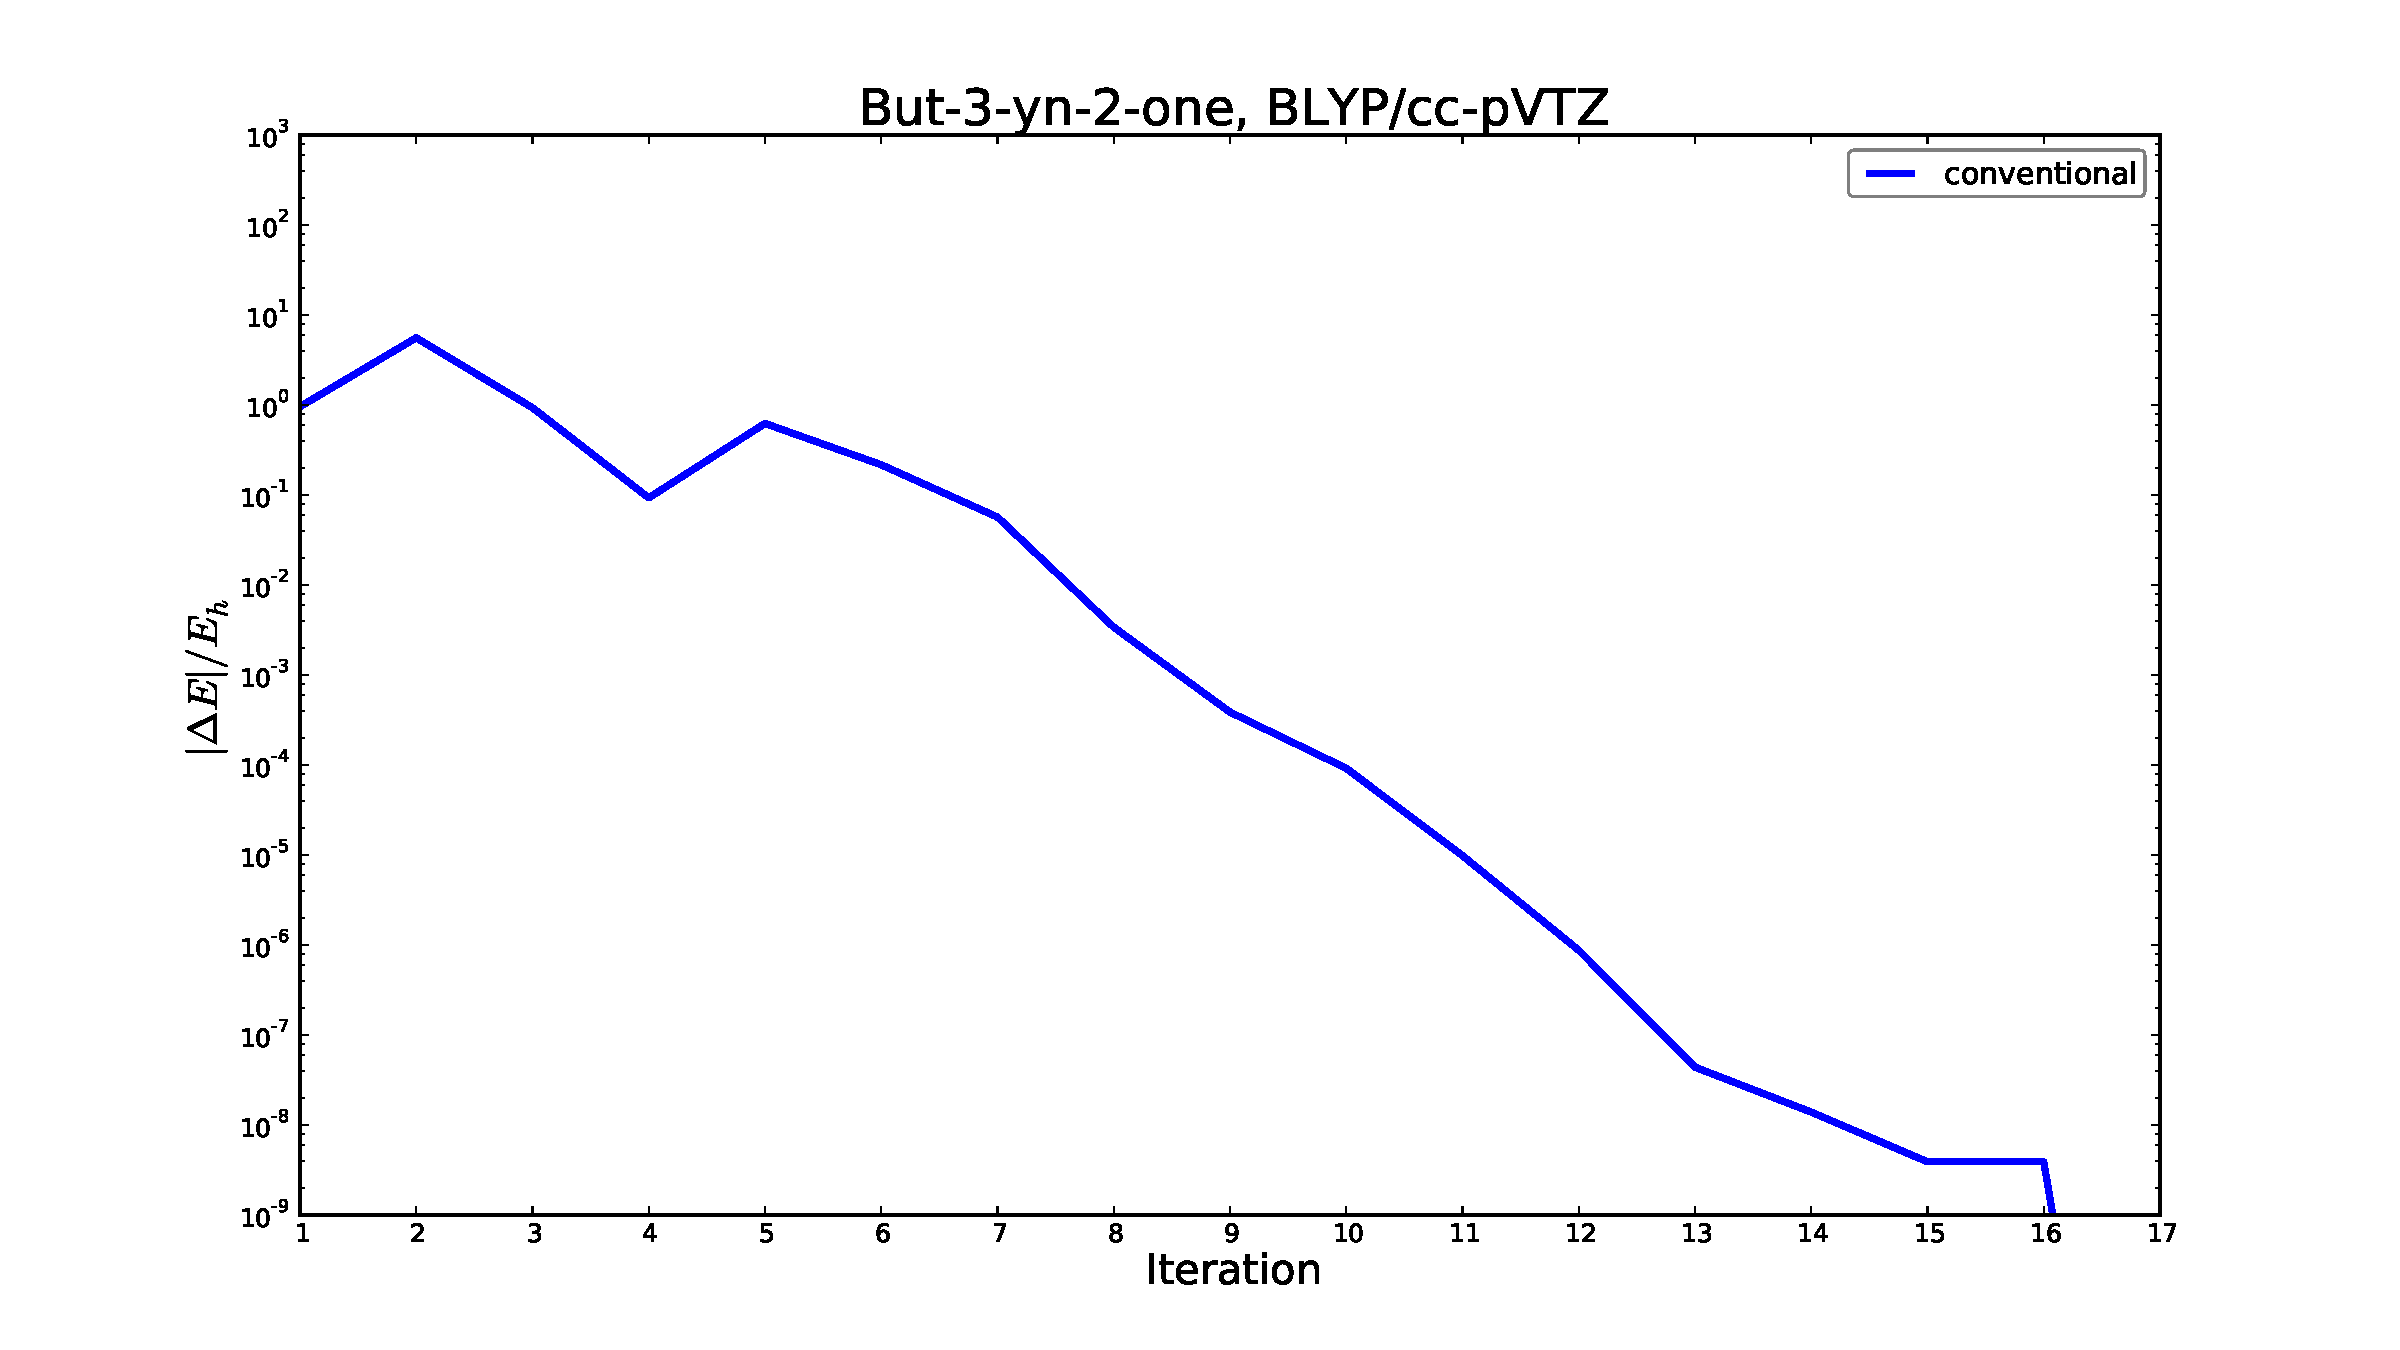
\includegraphics{Figures/conventional.pdf}
            }
        \end{figure}
    \end{center}
\end{frame}

\begin{frame}
   \frametitle{BLYP cc-pVTZ/cc-pVTZdenfit SCF iterations}
   \tiny{Development version of Molcas, www.molcas.org}
    \begin{center}
        \begin{figure}
            \scalebox{0.3}{
                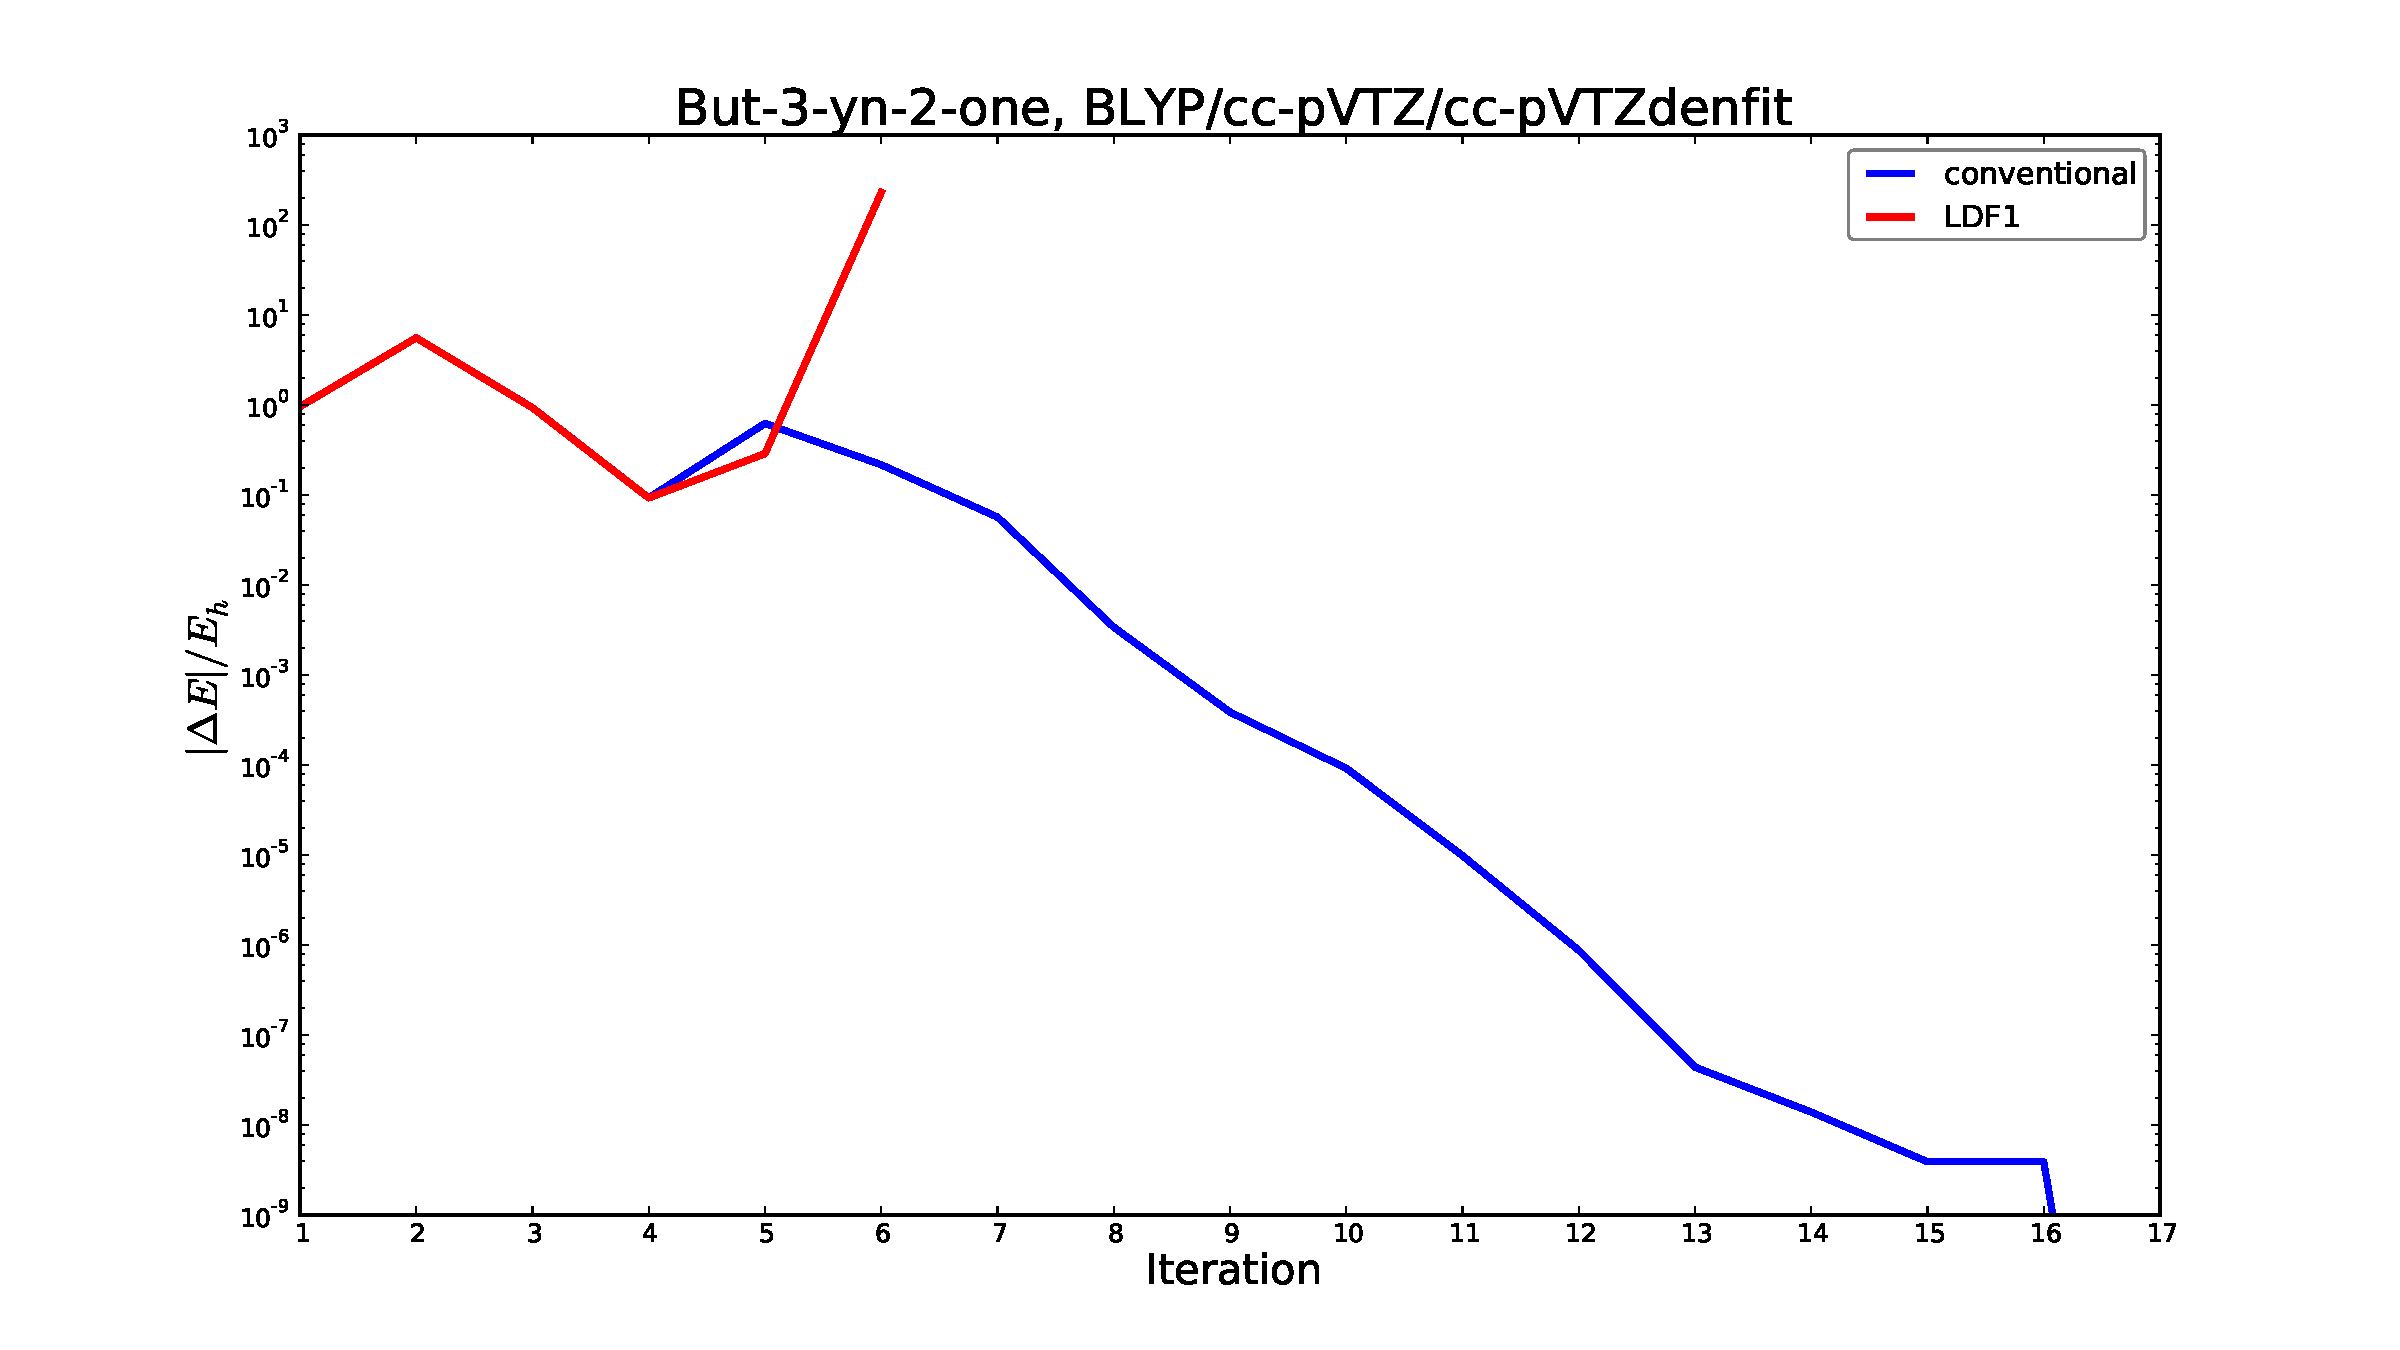
\includegraphics{Figures/conventional_ldf1.pdf}
            }
        \end{figure}
    \end{center}
\end{frame}

\begin{frame}
   \frametitle{BLYP cc-pVTZ/cc-pVTZdenfit SCF iterations}
   \tiny{Development version of Molcas, www.molcas.org}
    \begin{center}
        \begin{figure}
            \scalebox{0.3}{
                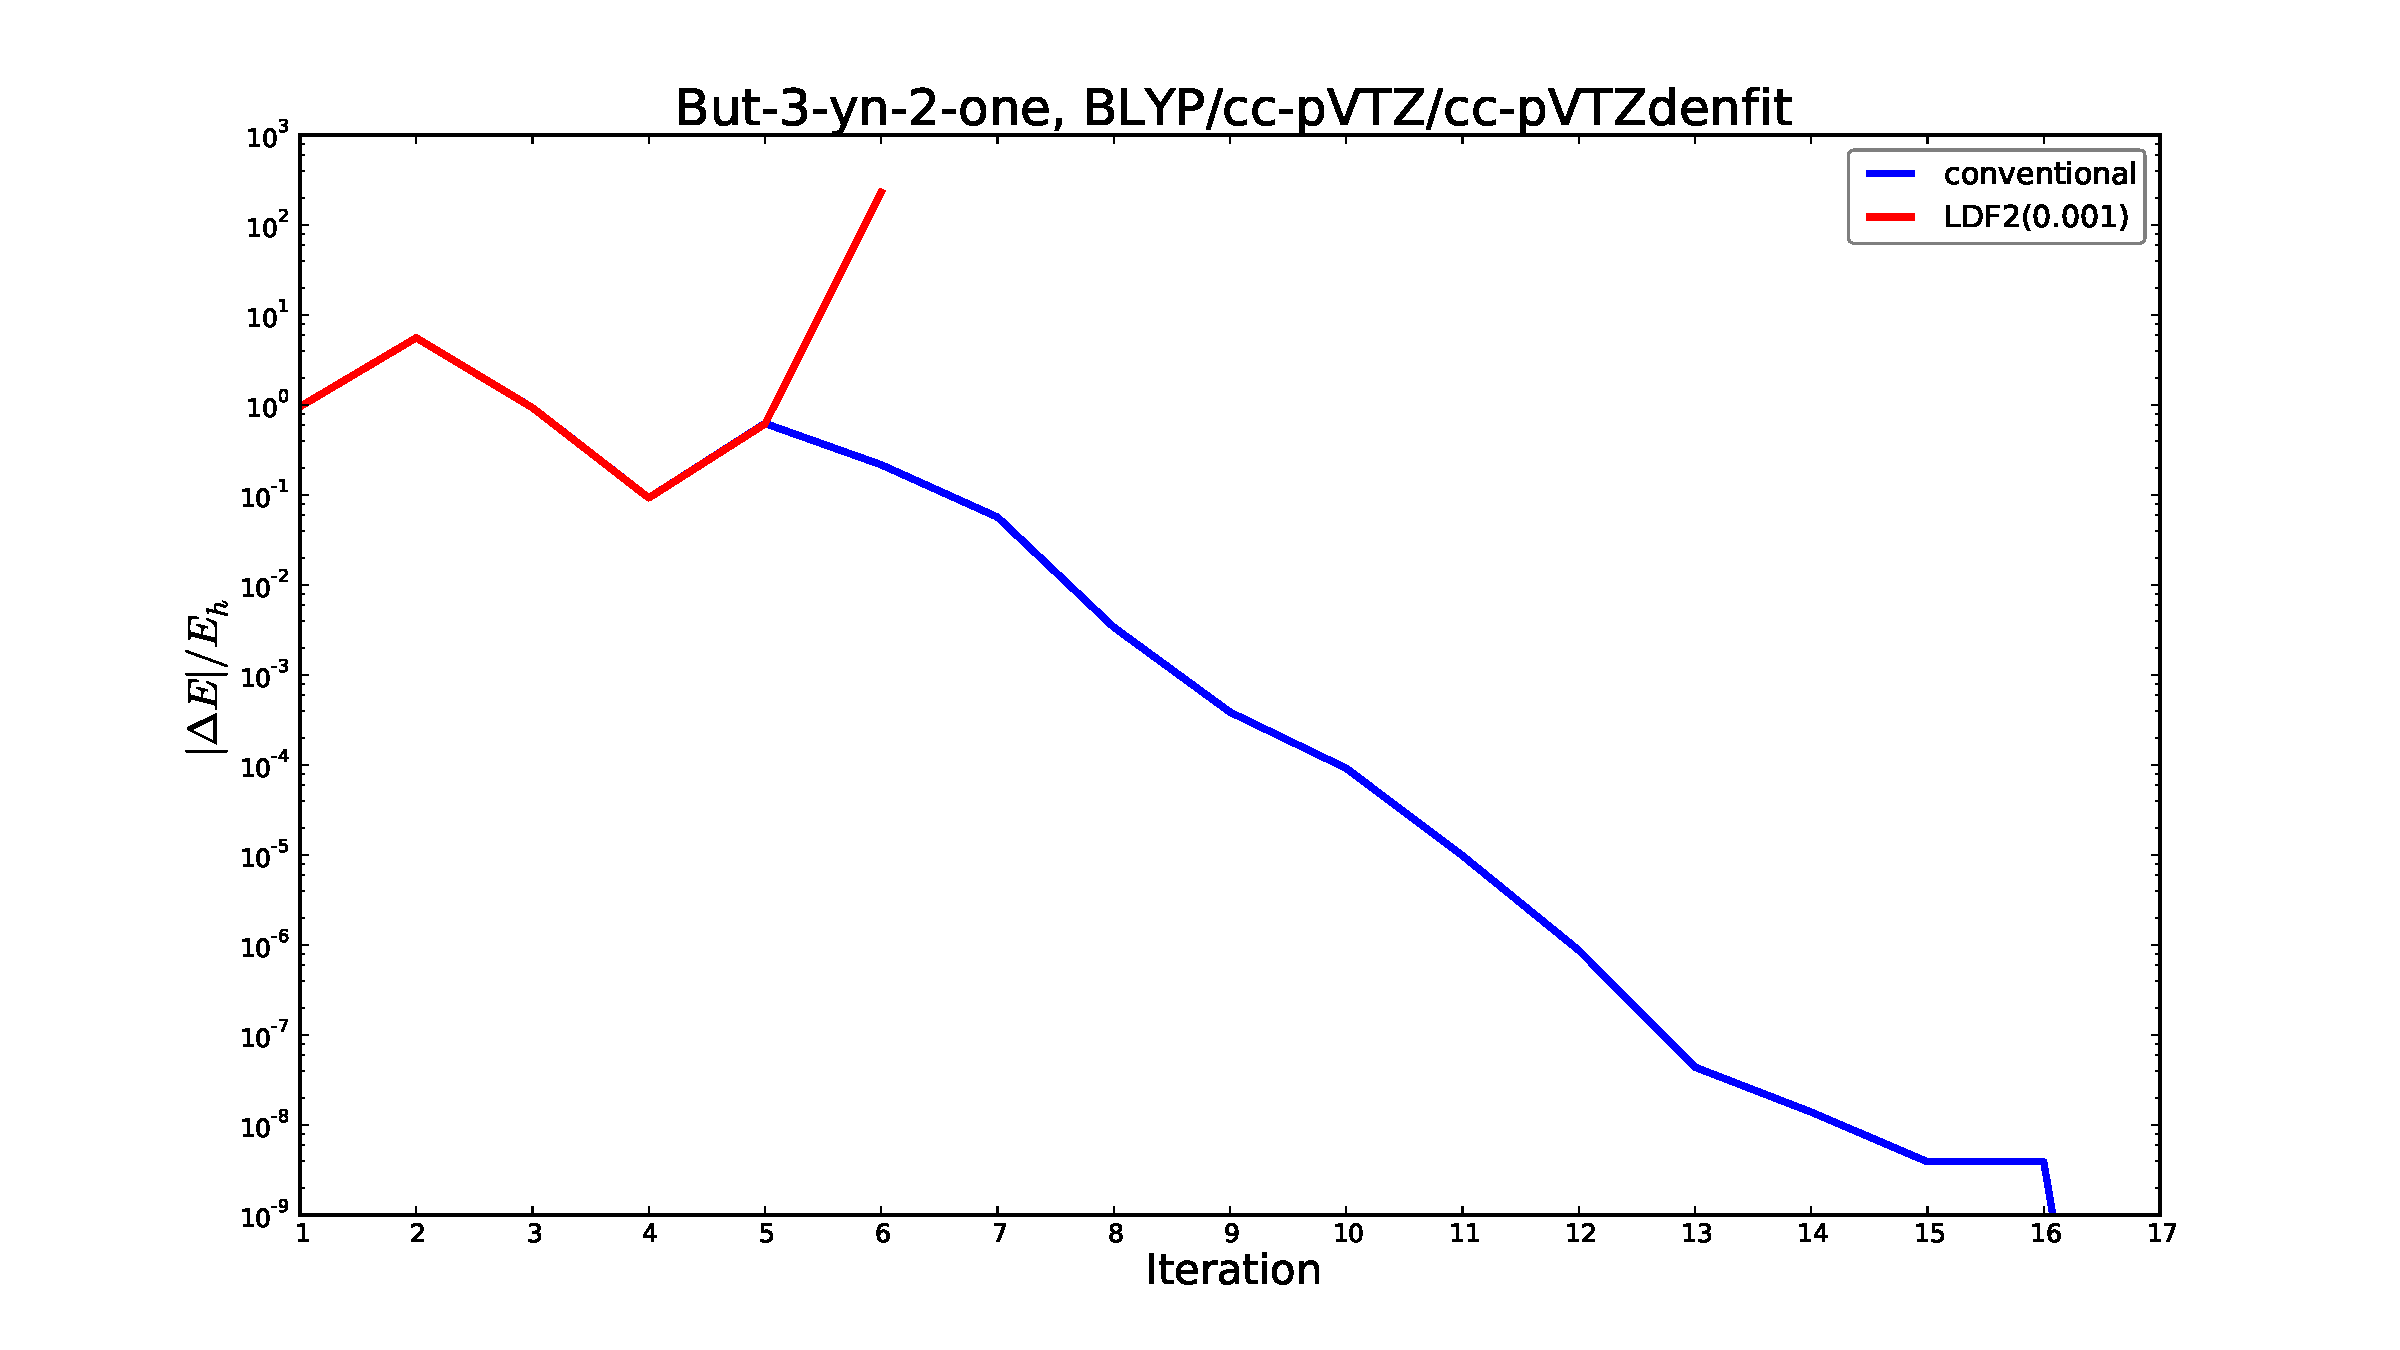
\includegraphics{Figures/conventional_ldf2_3.pdf}
            }
        \end{figure}
    \end{center}
\end{frame}

\begin{frame}
   \frametitle{BLYP cc-pVTZ/cc-pVTZdenfit SCF iterations}
   \tiny{Development version of Molcas, www.molcas.org}
    \begin{center}
        \begin{figure}
            \scalebox{0.3}{
                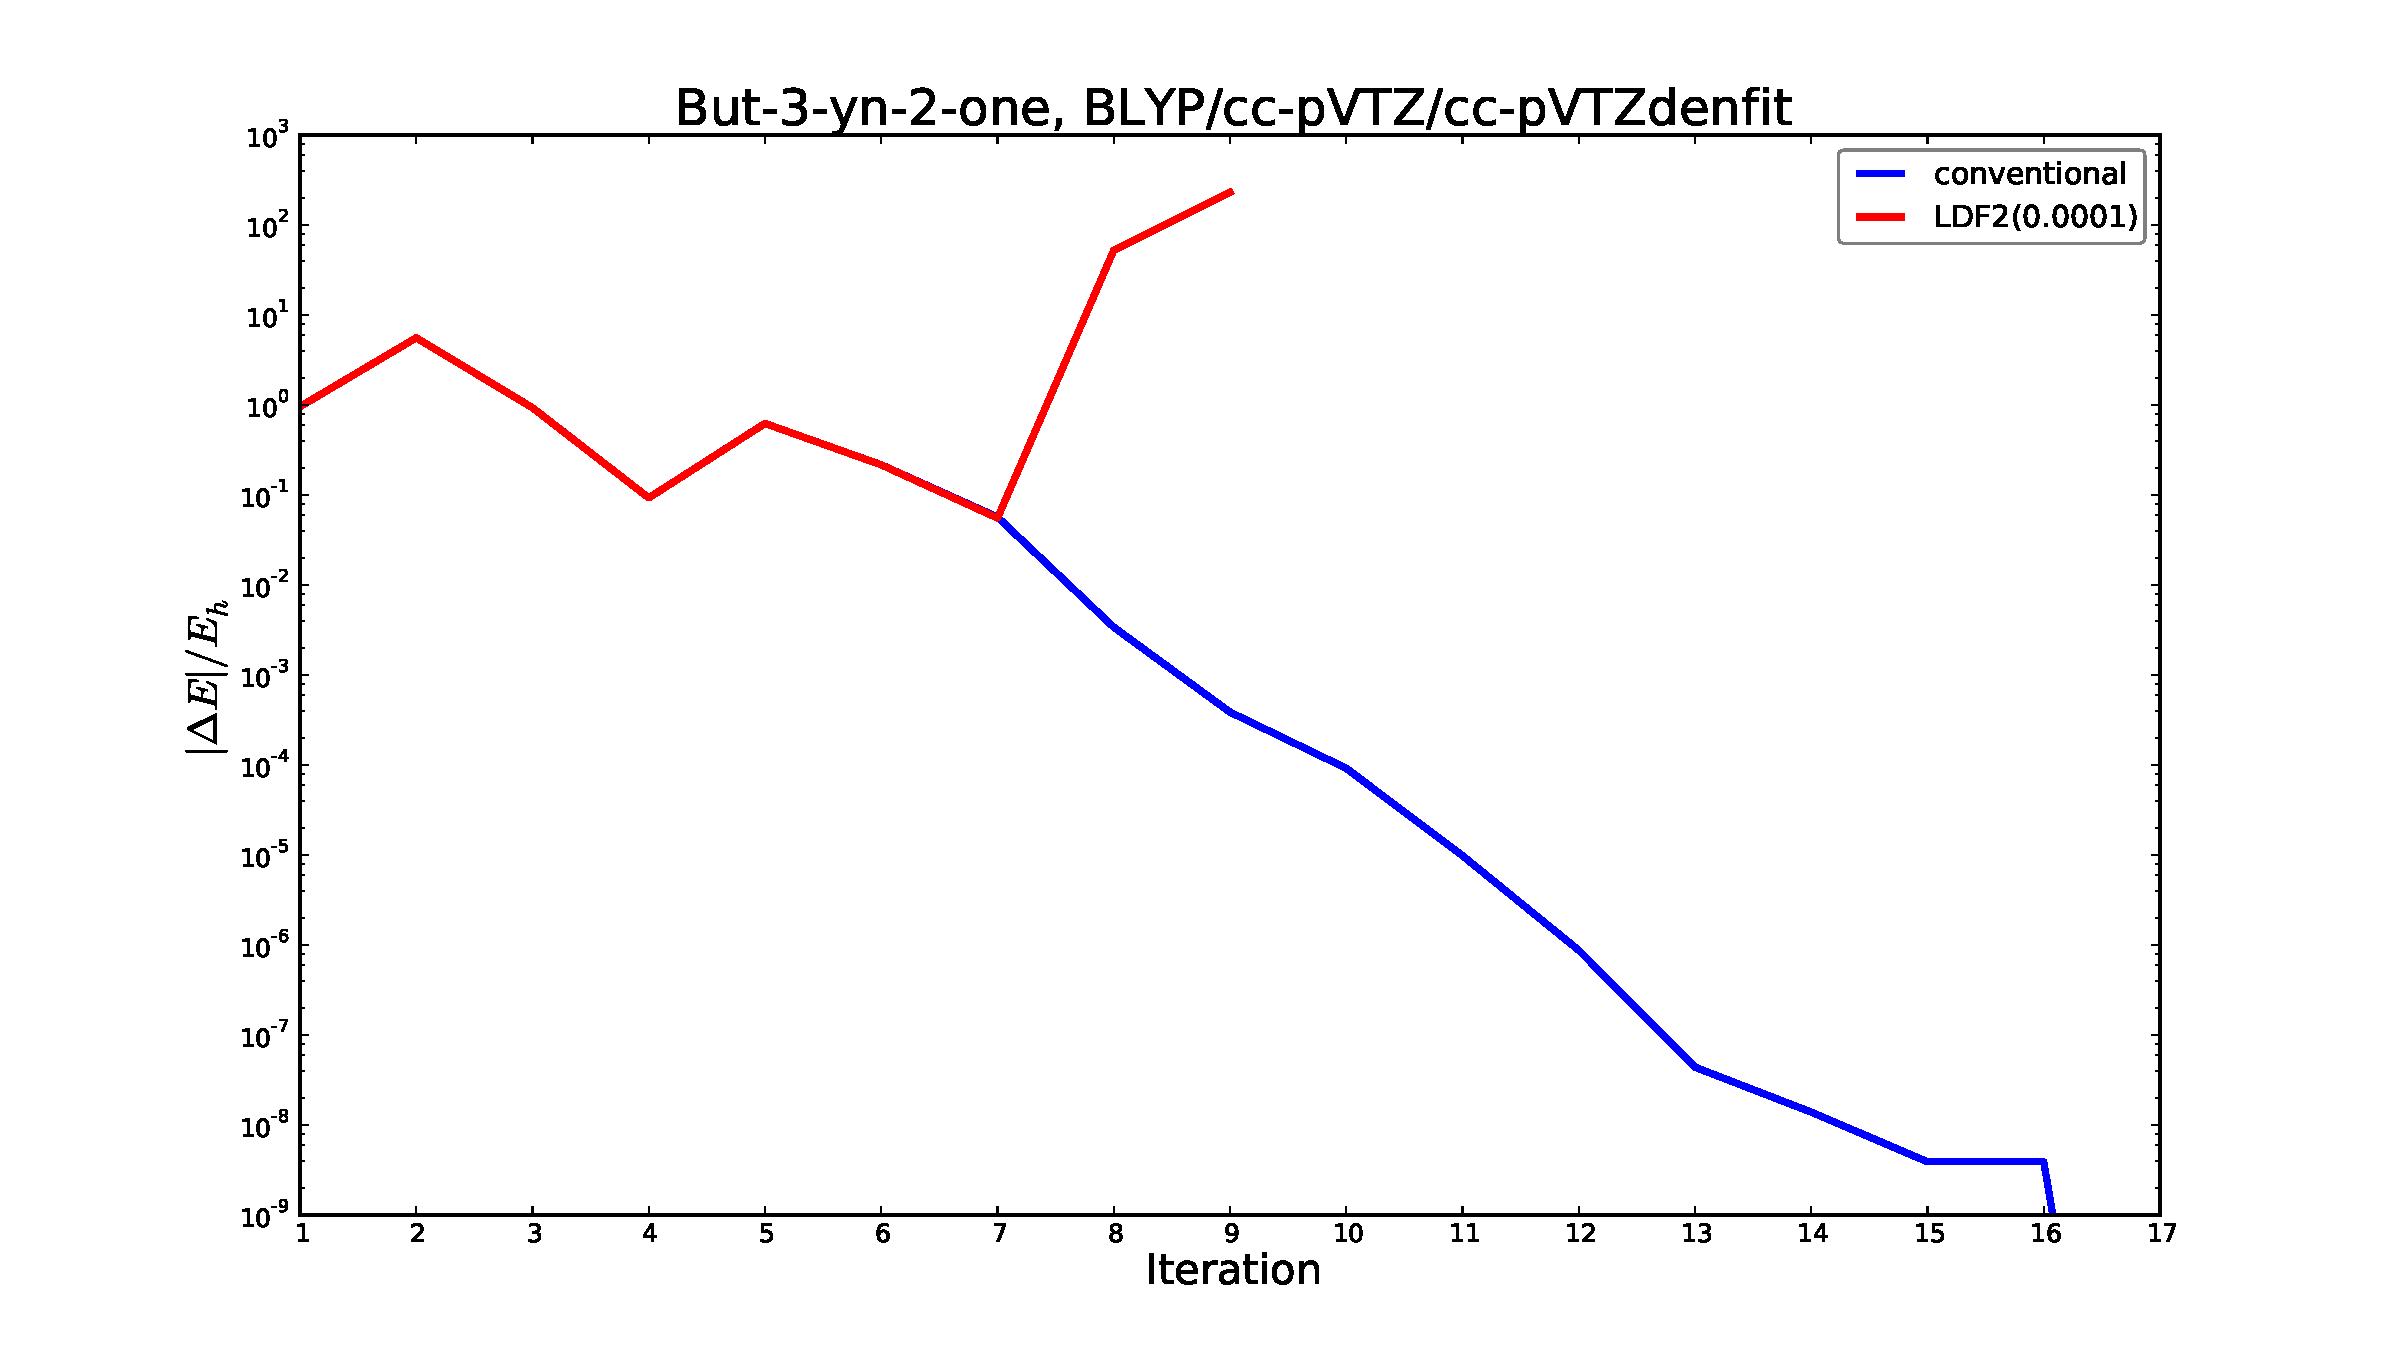
\includegraphics{Figures/conventional_ldf2_4.pdf}
            }
        \end{figure}
    \end{center}
\end{frame}

\begin{frame}
   \frametitle{BLYP cc-pVTZ/cc-pVTZdenfit SCF iterations}
   \tiny{Development version of Molcas, www.molcas.org}
    \begin{center}
        \begin{figure}
            \scalebox{0.3}{
                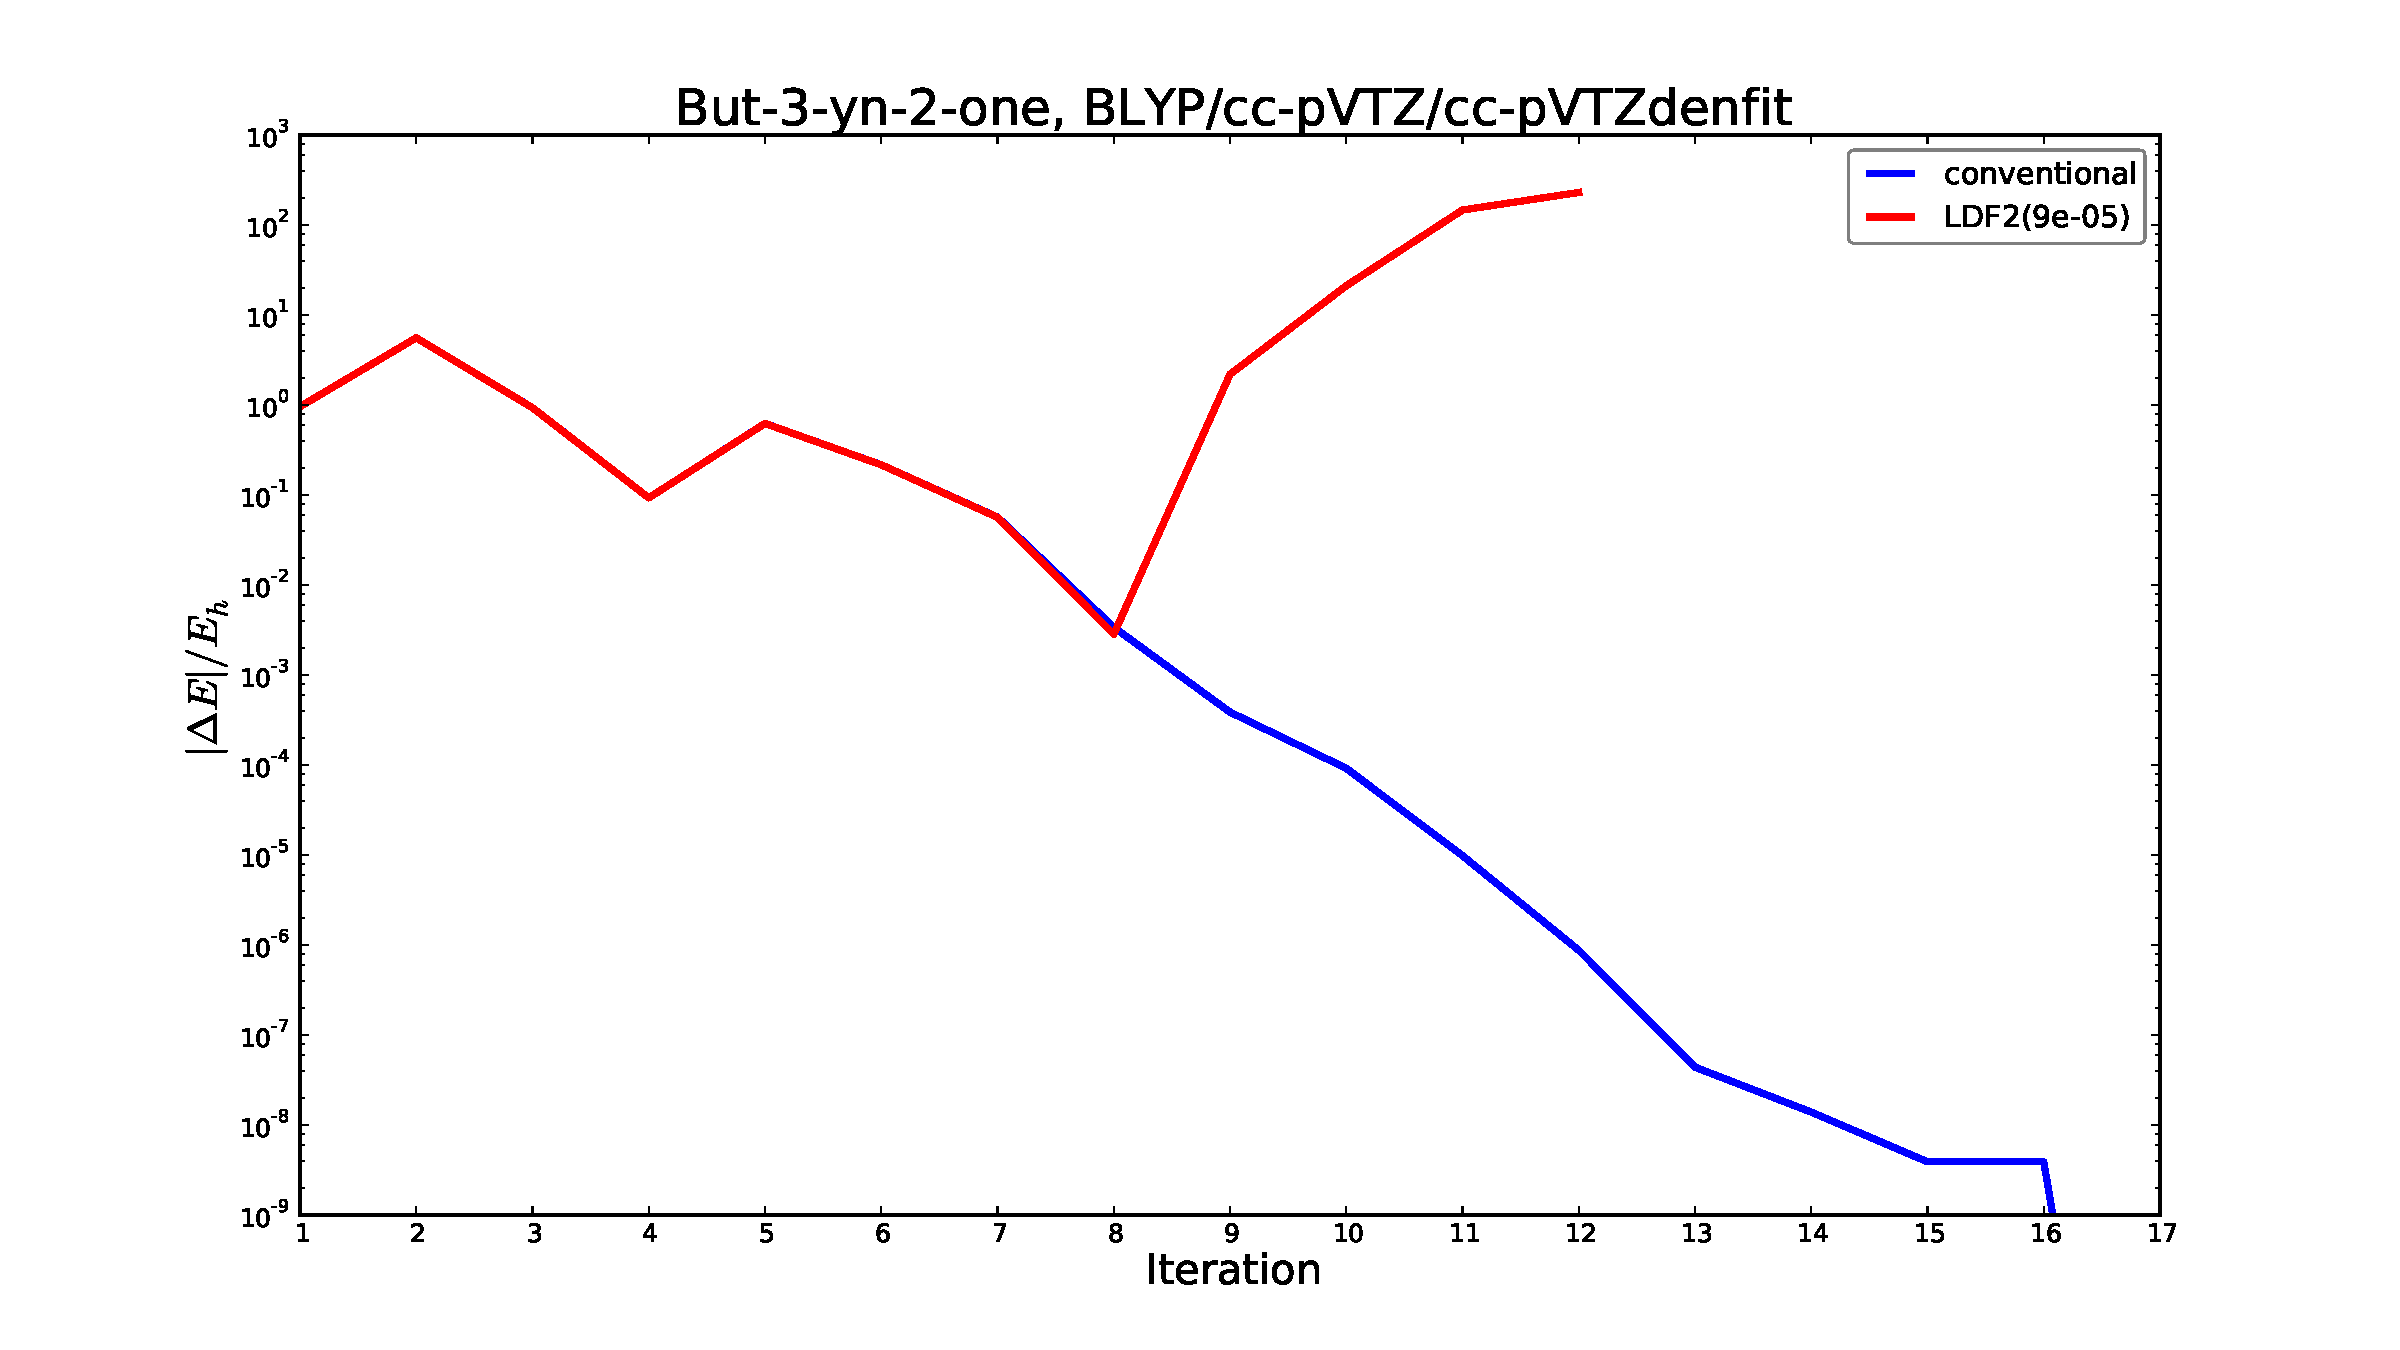
\includegraphics{Figures/conventional_ldf2_5_t9.pdf}
            }
        \end{figure}
    \end{center}
\end{frame}

\begin{frame}
   \frametitle{BLYP cc-pVTZ/cc-pVTZdenfit SCF iterations}
   \tiny{Development version of Molcas, www.molcas.org}
    \begin{center}
        \begin{figure}
            \scalebox{0.3}{
                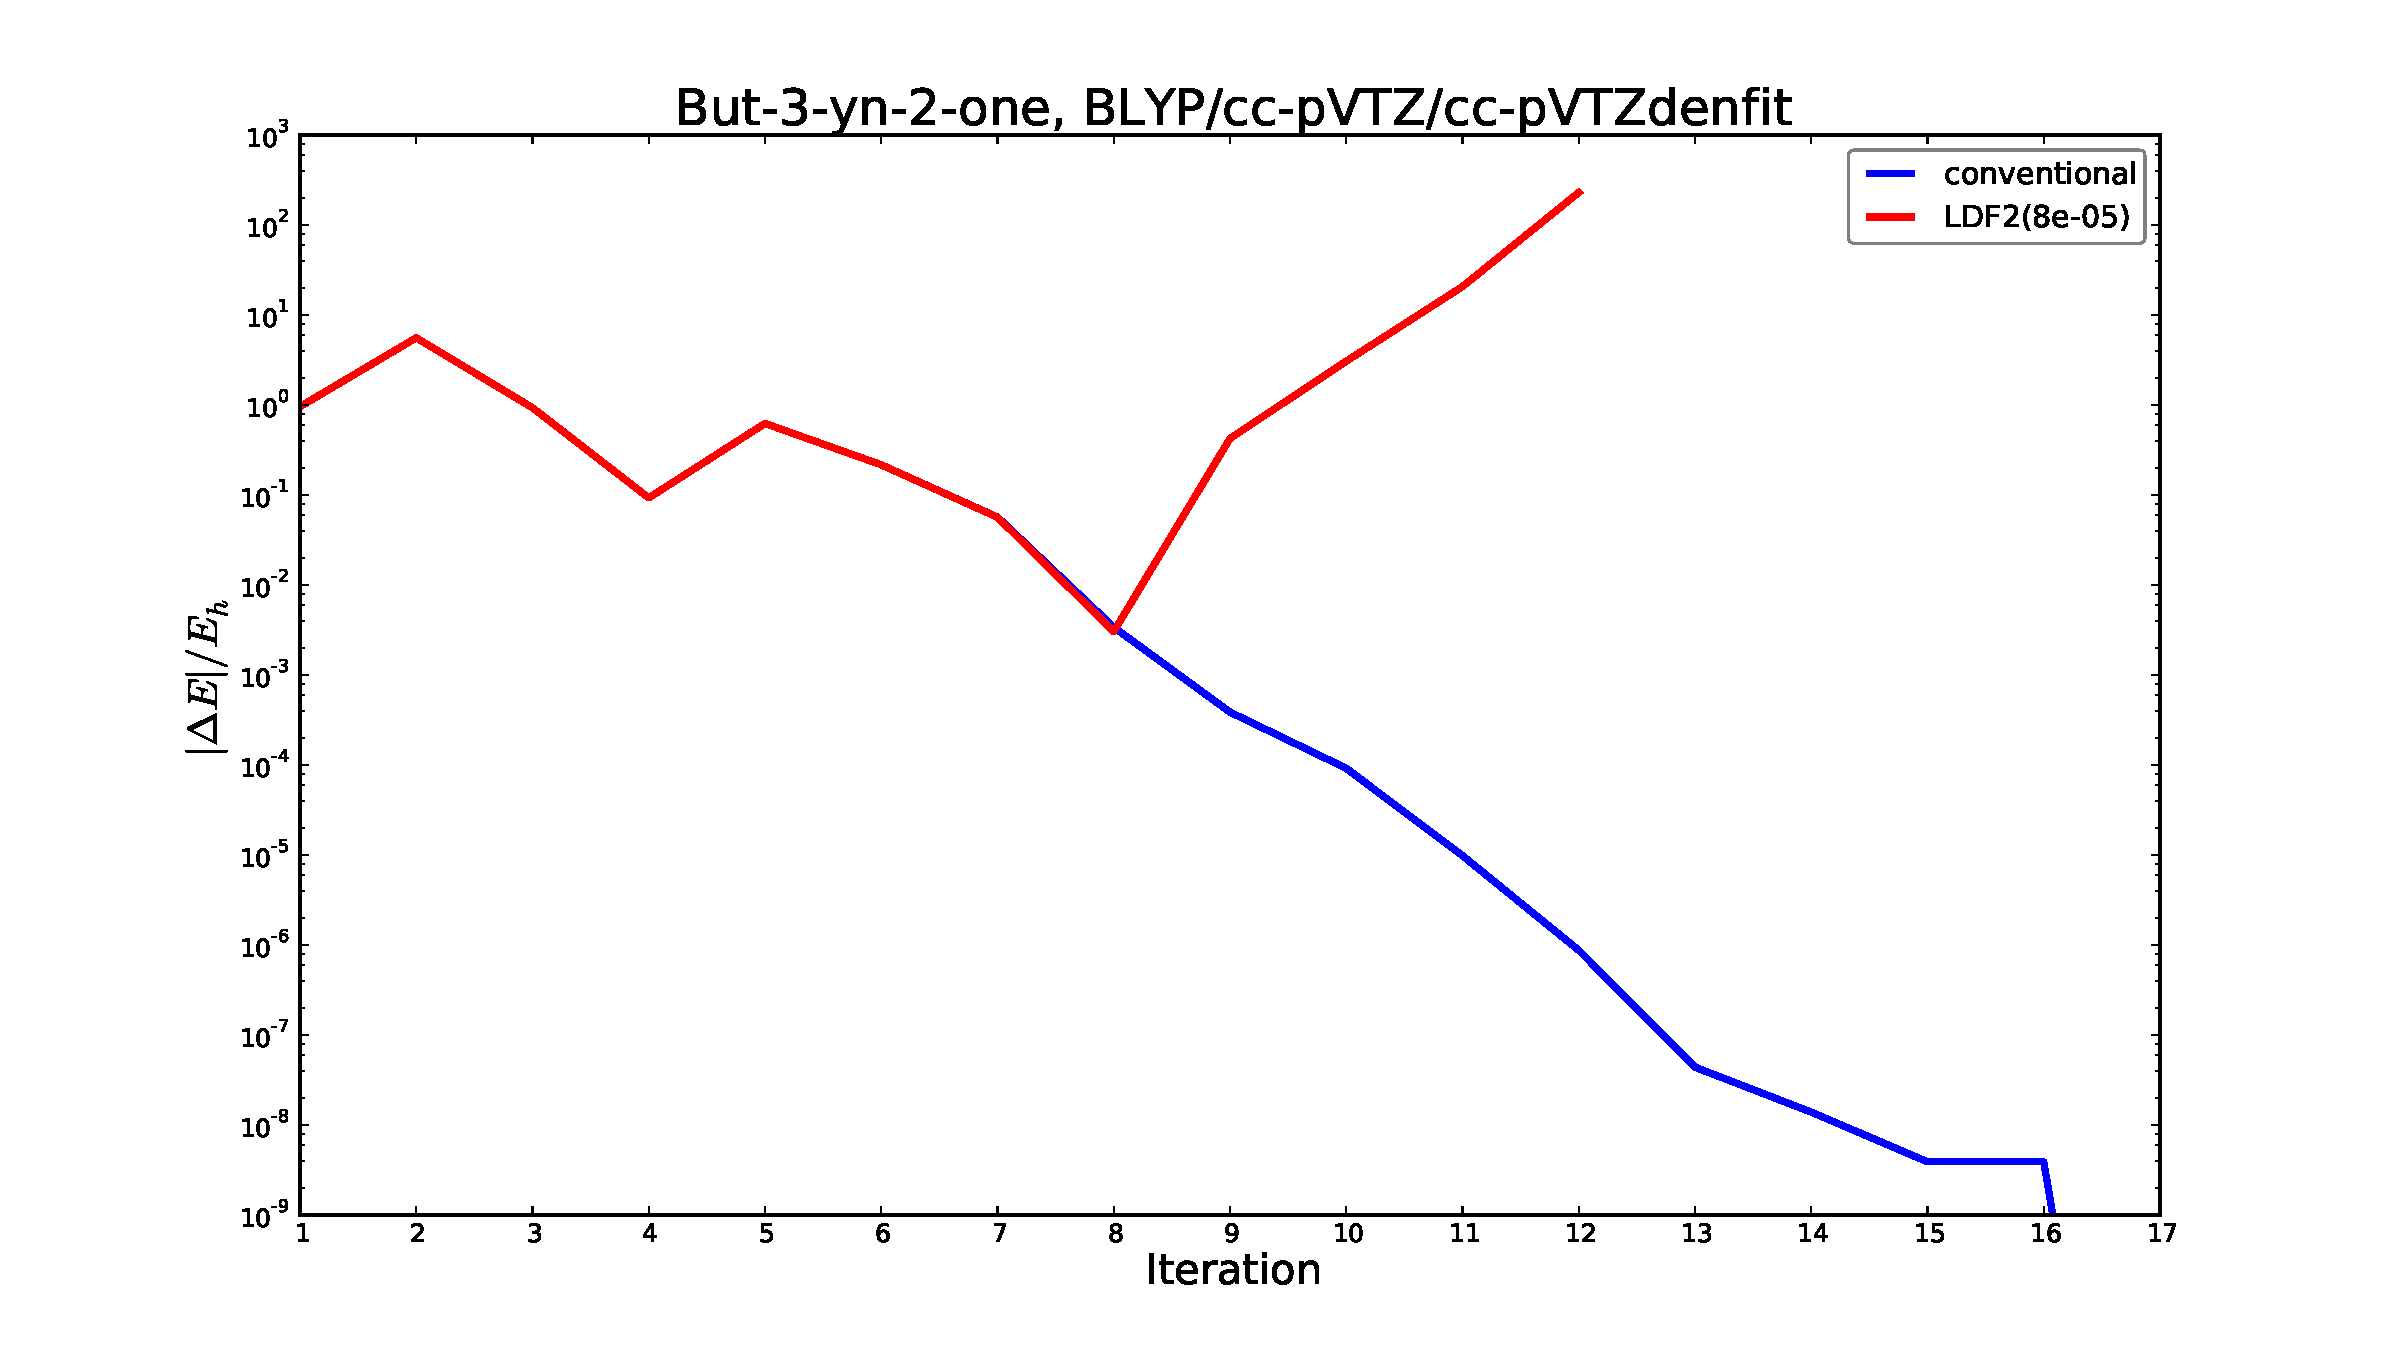
\includegraphics{Figures/conventional_ldf2_5_t8.pdf}
            }
        \end{figure}
    \end{center}
\end{frame}

\begin{frame}
   \frametitle{BLYP cc-pVTZ/cc-pVTZdenfit SCF iterations}
   \tiny{Development version of Molcas, www.molcas.org}
    \begin{center}
        \begin{figure}
            \scalebox{0.3}{
                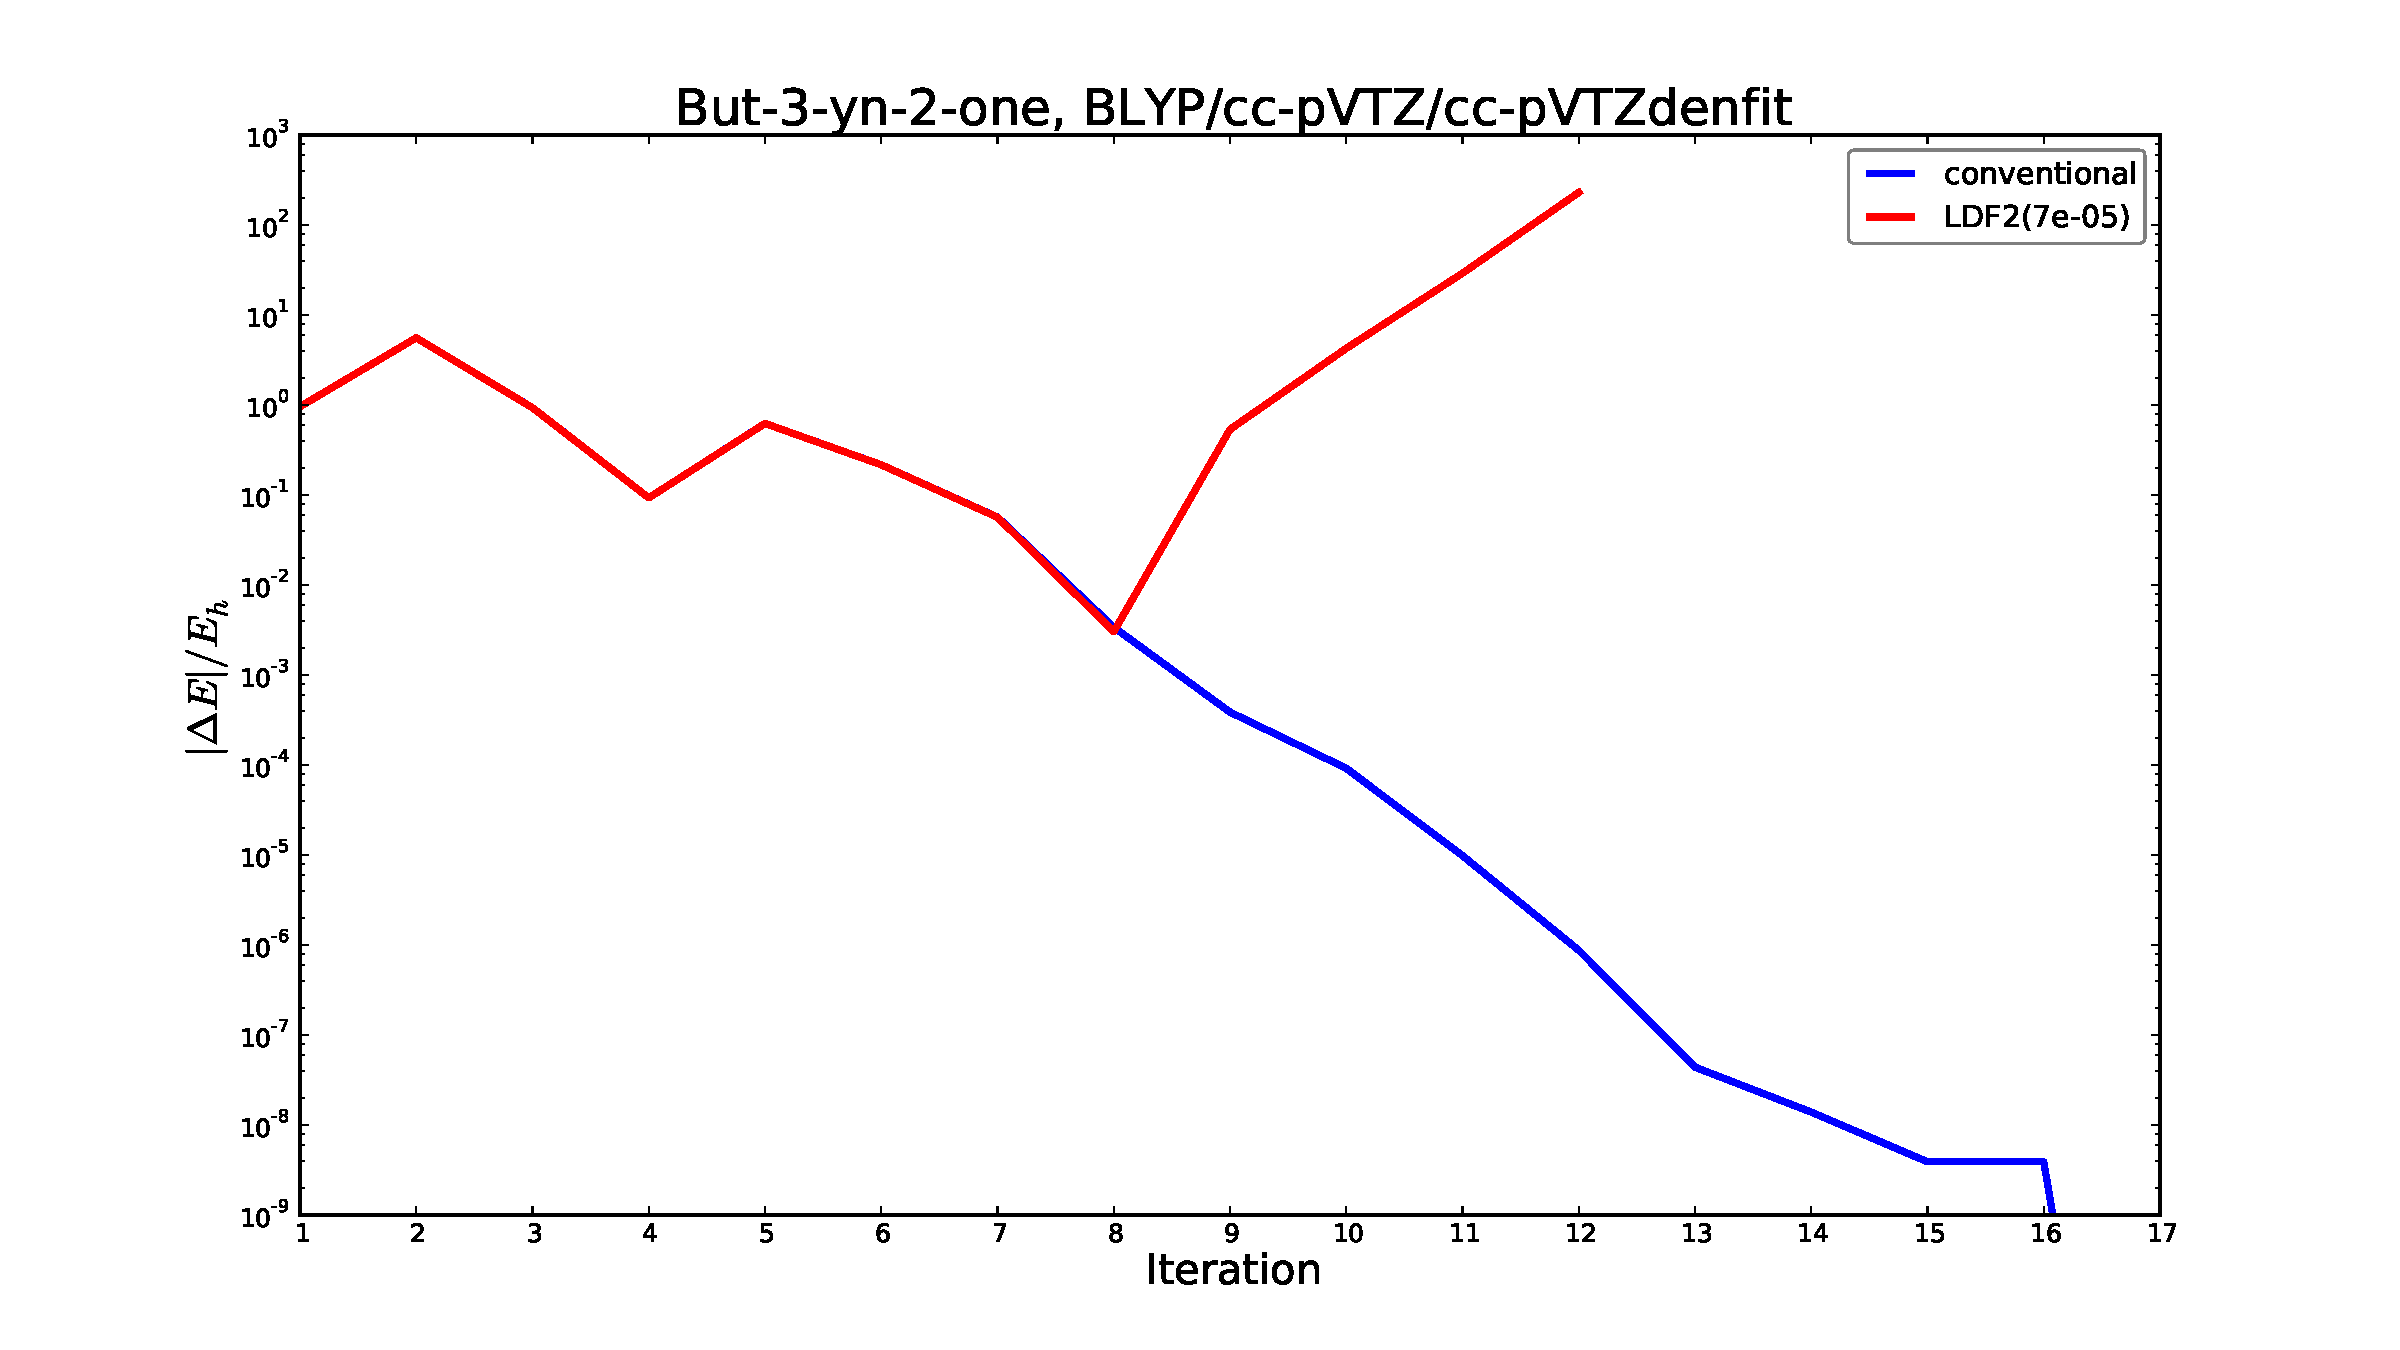
\includegraphics{Figures/conventional_ldf2_5_t7.pdf}
            }
        \end{figure}
    \end{center}
\end{frame}

\begin{frame}
   \frametitle{BLYP cc-pVTZ/cc-pVTZdenfit SCF iterations}
   \tiny{Development version of Molcas, www.molcas.org}
    \begin{center}
        \begin{figure}
            \scalebox{0.3}{
                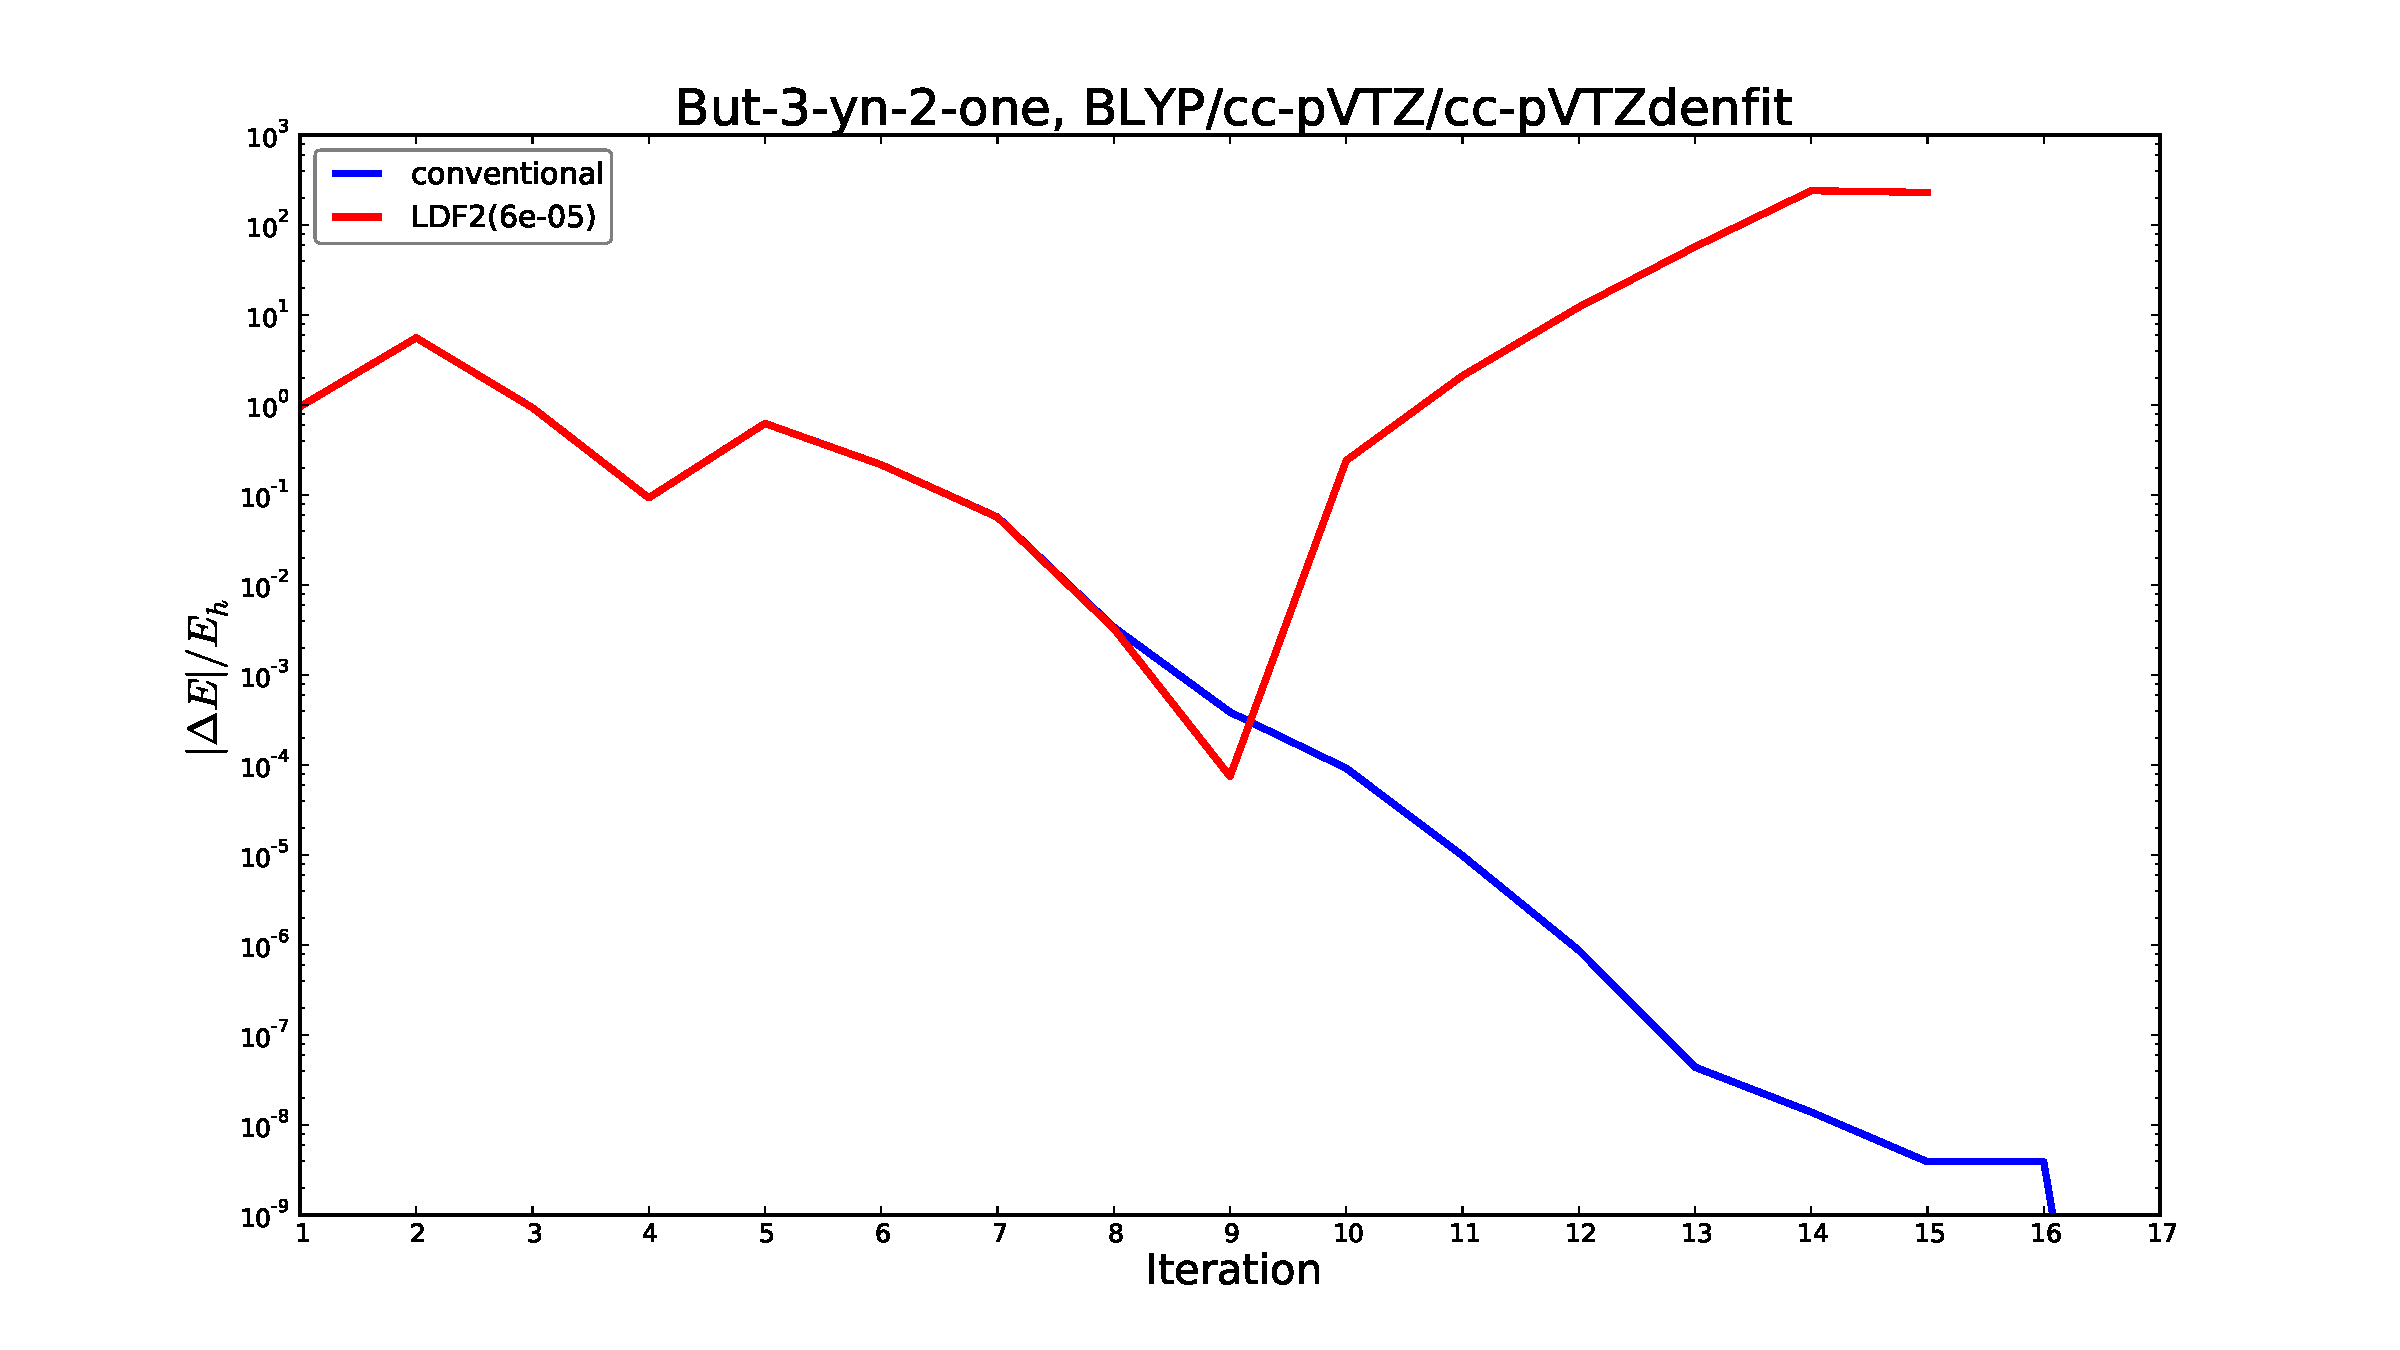
\includegraphics{Figures/conventional_ldf2_5_t6.pdf}
            }
        \end{figure}
    \end{center}
\end{frame}

\begin{frame}
   \frametitle{BLYP cc-pVTZ/cc-pVTZdenfit SCF iterations}
   \tiny{Development version of Molcas, www.molcas.org}
    \begin{center}
        \begin{figure}
            \scalebox{0.3}{
                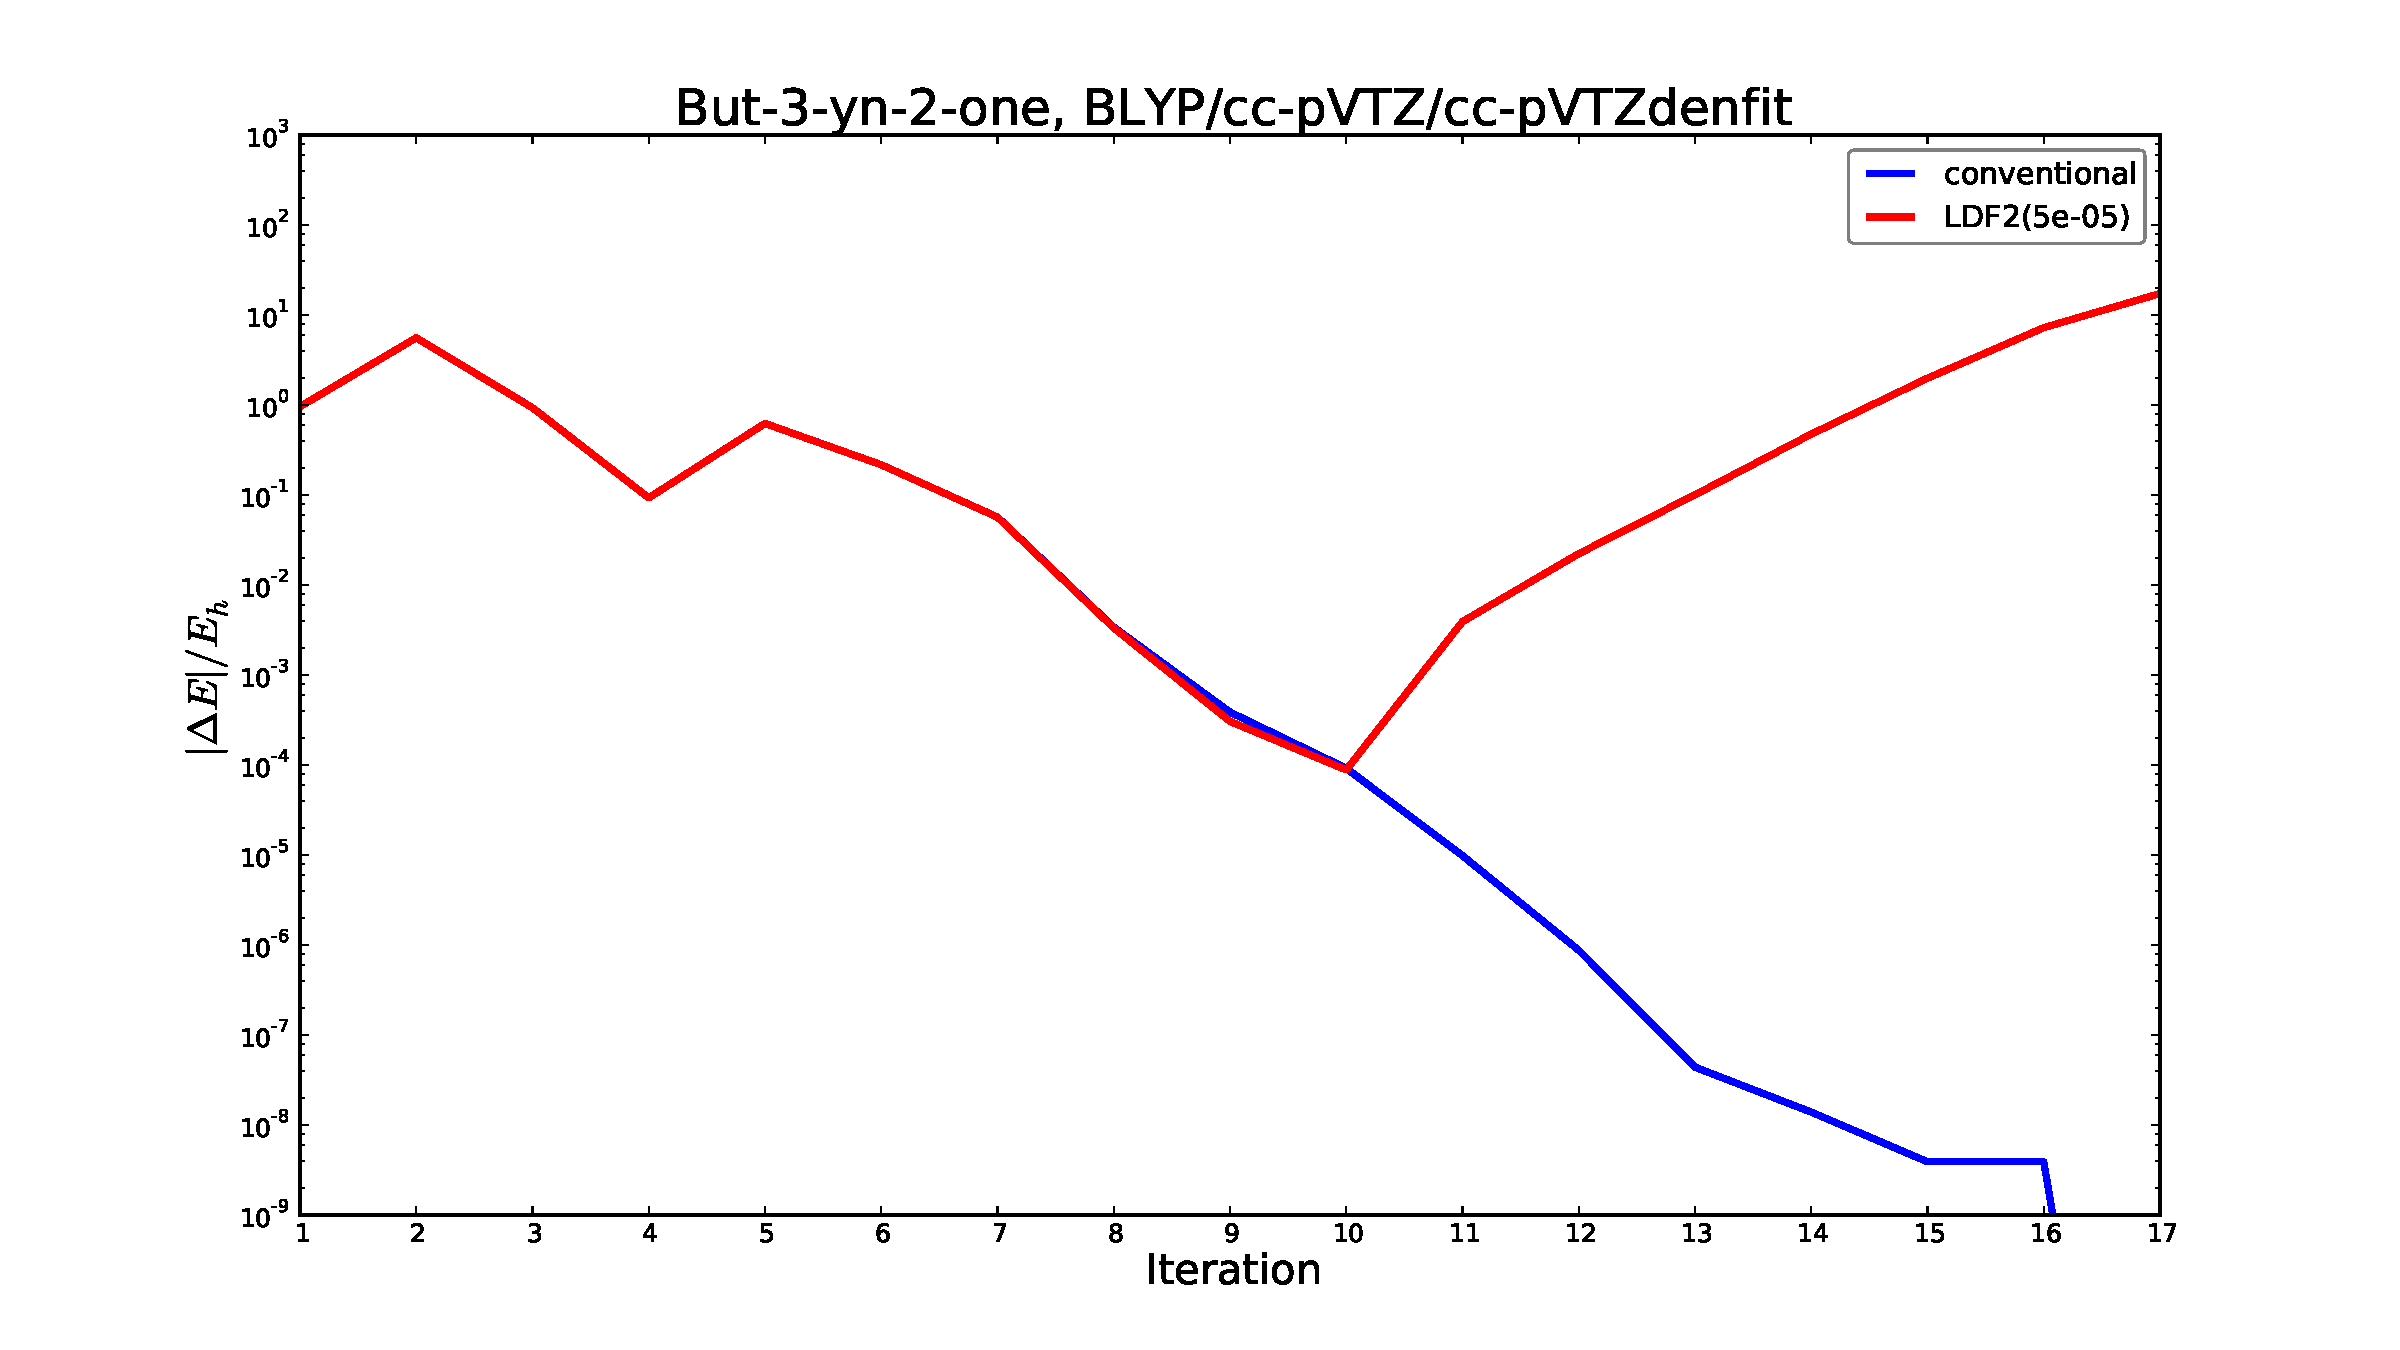
\includegraphics{Figures/conventional_ldf2_5_t5.pdf}
            }
        \end{figure}
    \end{center}
\end{frame}

\begin{frame}
   \frametitle{BLYP cc-pVTZ/cc-pVTZdenfit SCF iterations}
   \tiny{Development version of Molcas, www.molcas.org}
    \begin{center}
        \begin{figure}
            \scalebox{0.3}{
                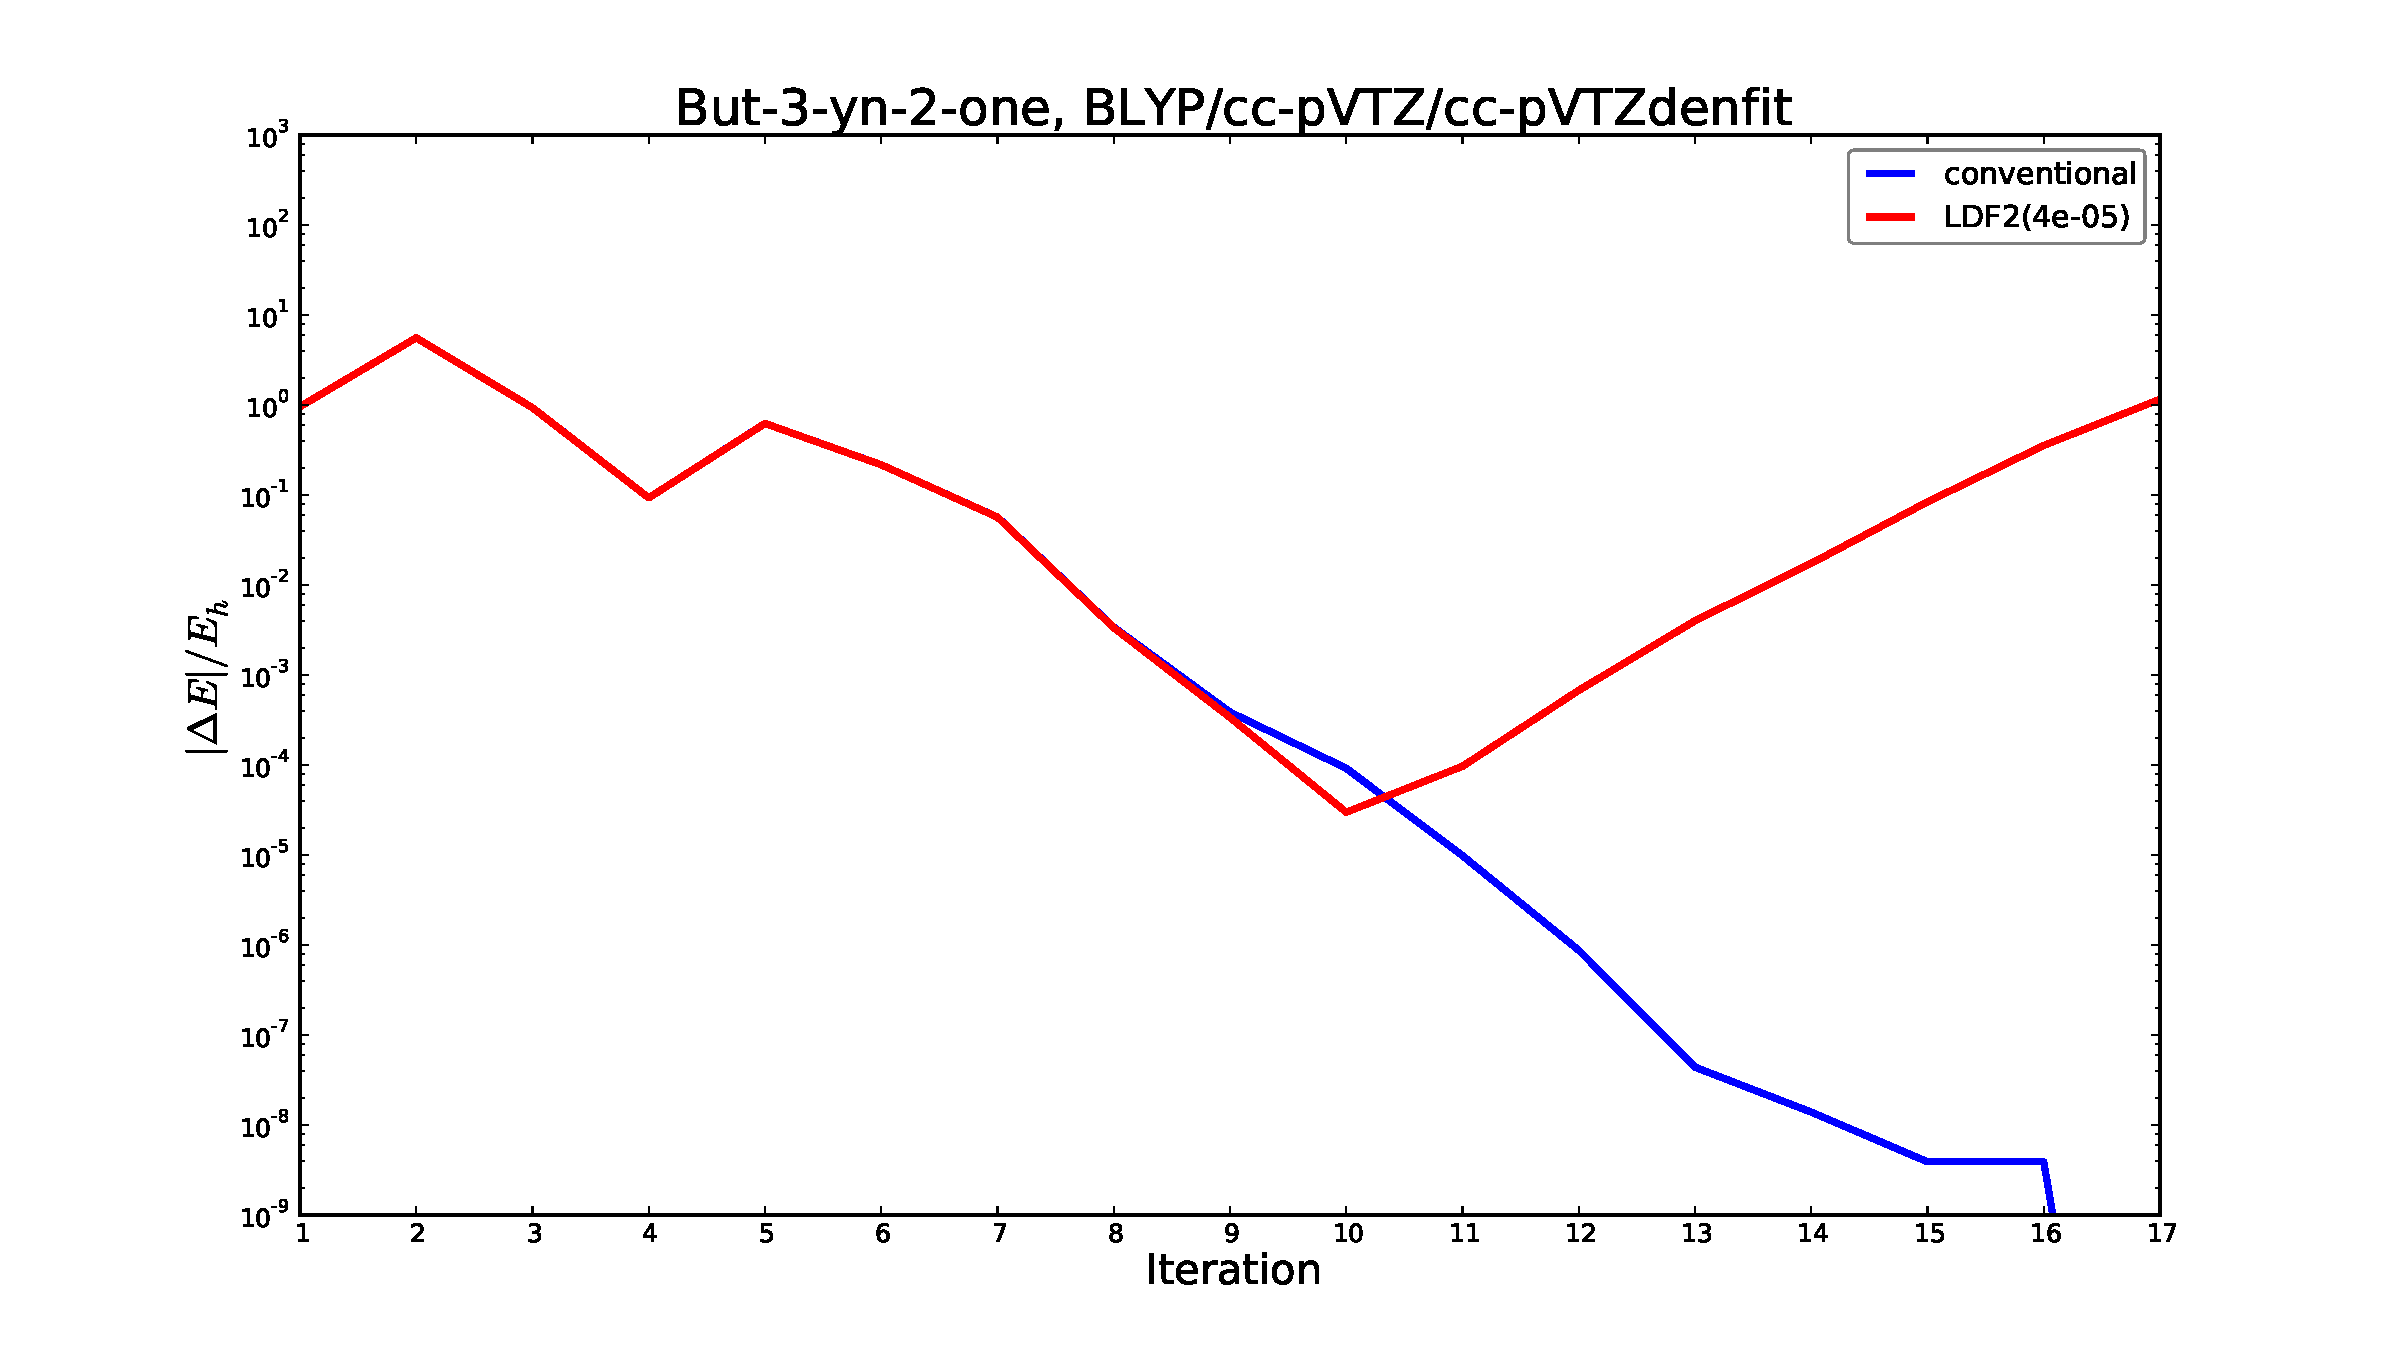
\includegraphics{Figures/conventional_ldf2_5_t4.pdf}
            }
        \end{figure}
    \end{center}
\end{frame}

\begin{frame}
   \frametitle{BLYP cc-pVTZ/cc-pVTZdenfit SCF iterations}
   \tiny{Development version of Molcas, www.molcas.org}
    \begin{center}
        \begin{figure}
            \scalebox{0.3}{
                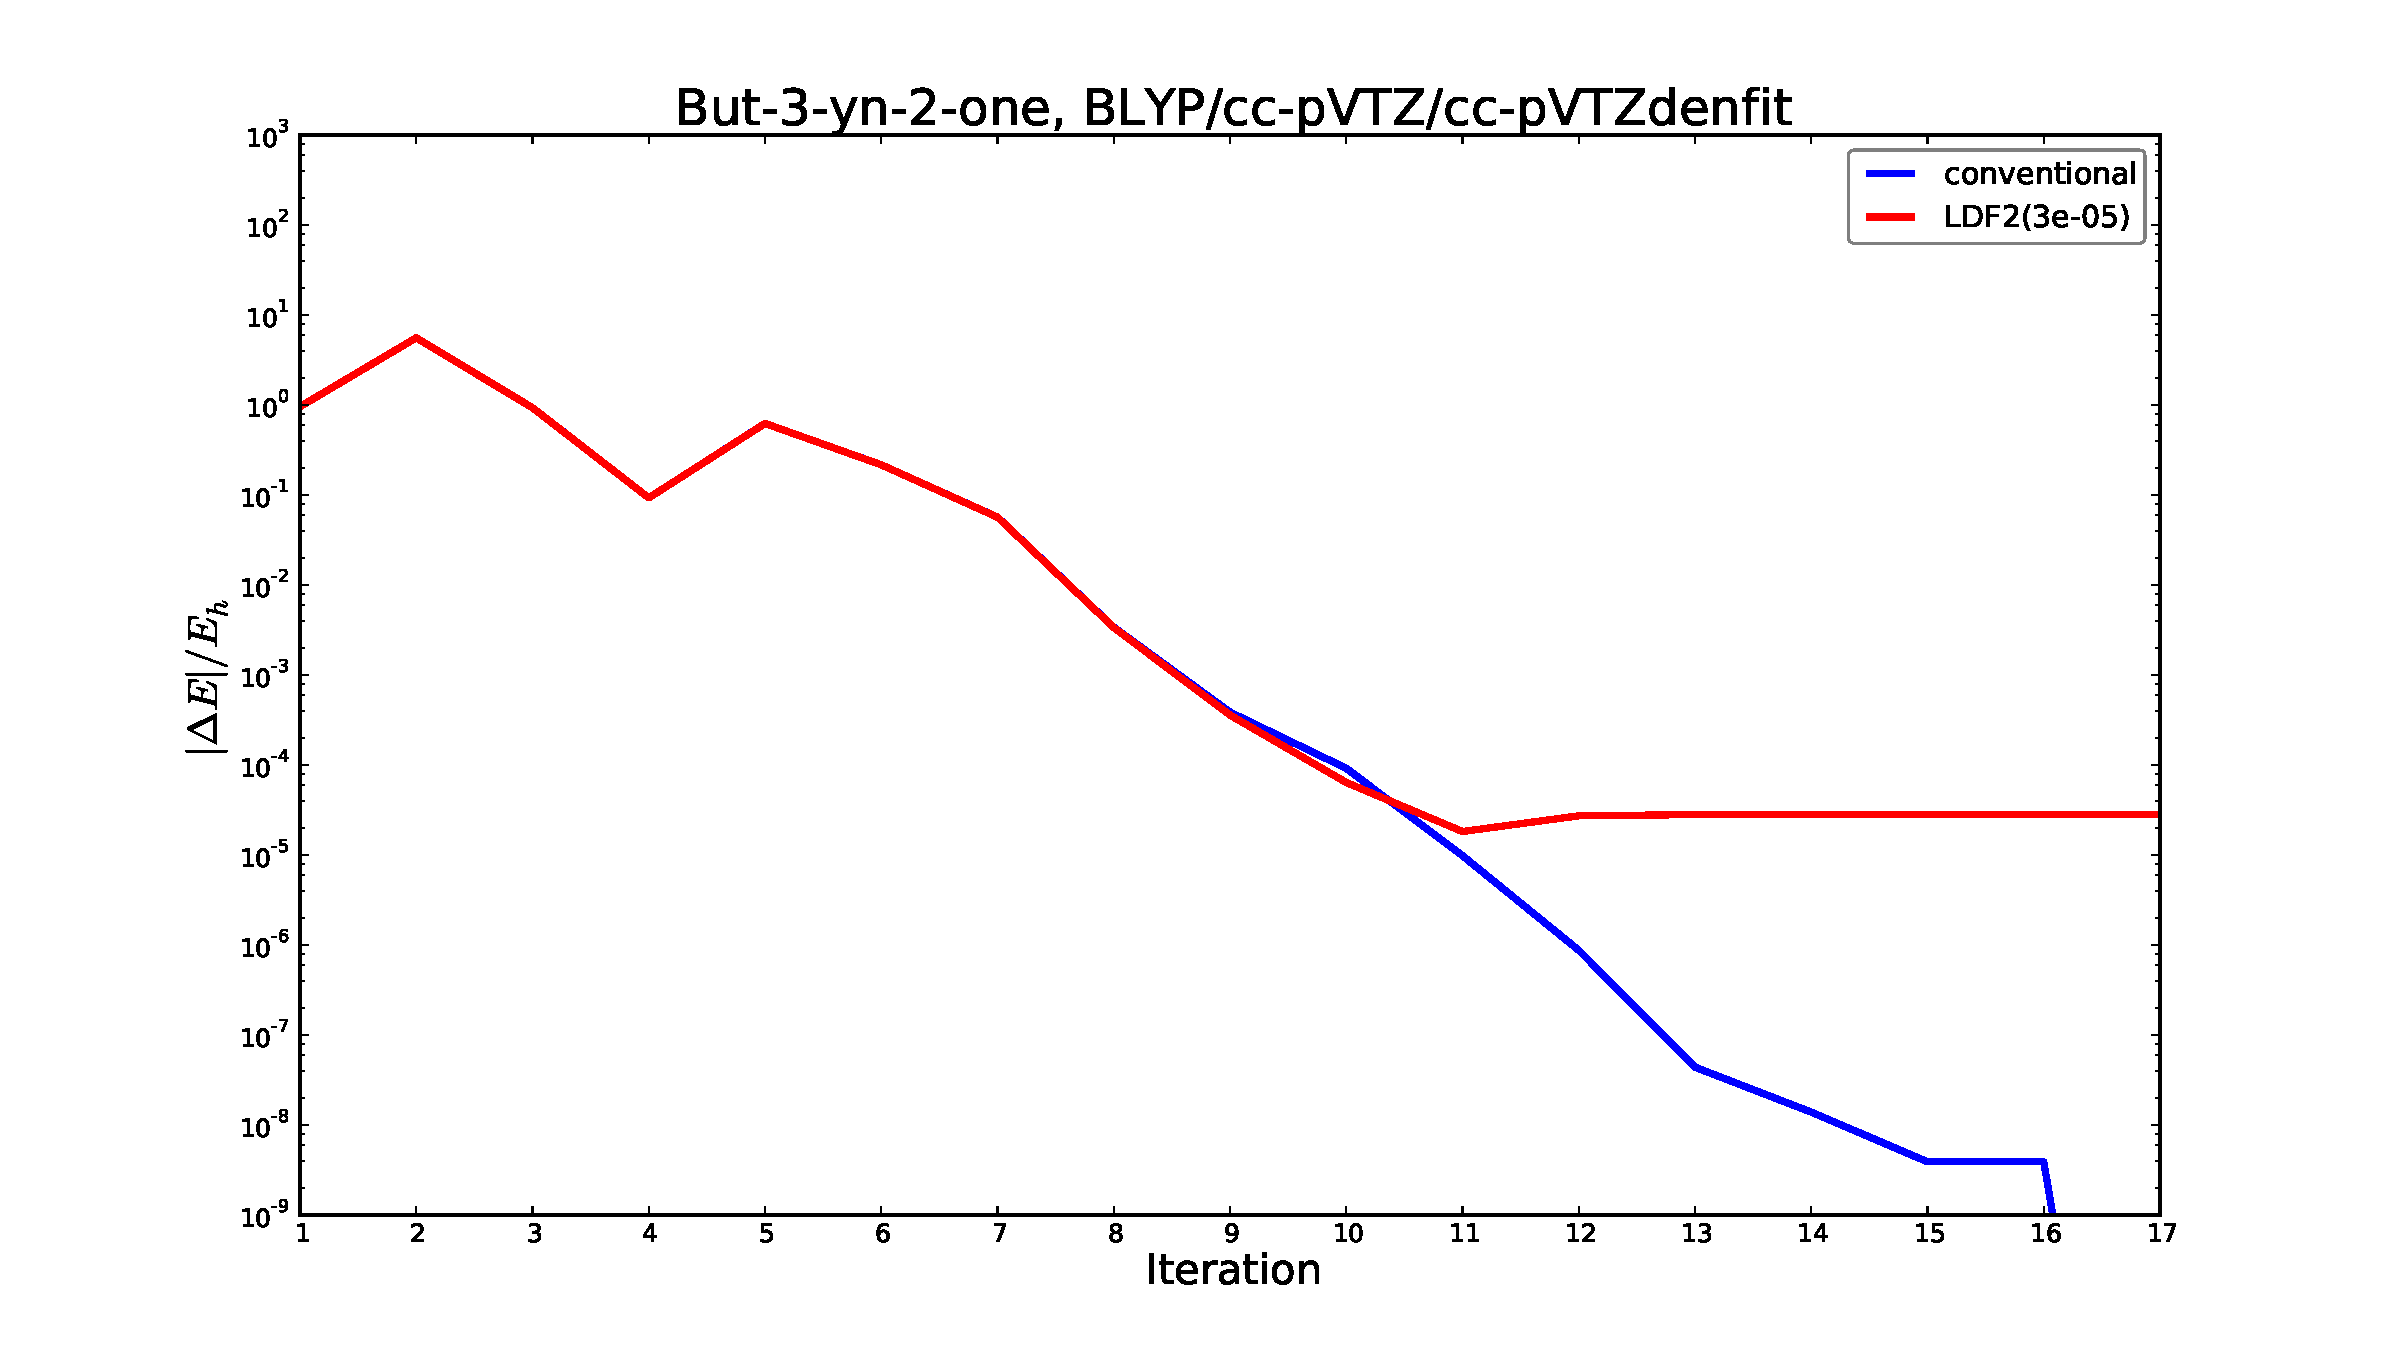
\includegraphics{Figures/conventional_ldf2_5_t3.pdf}
            }
        \end{figure}
    \end{center}
\end{frame}

\begin{frame}
   \frametitle{BLYP cc-pVTZ/cc-pVTZdenfit SCF iterations}
   \tiny{Development version of Molcas, www.molcas.org}
    \begin{center}
        \begin{figure}
            \scalebox{0.3}{
                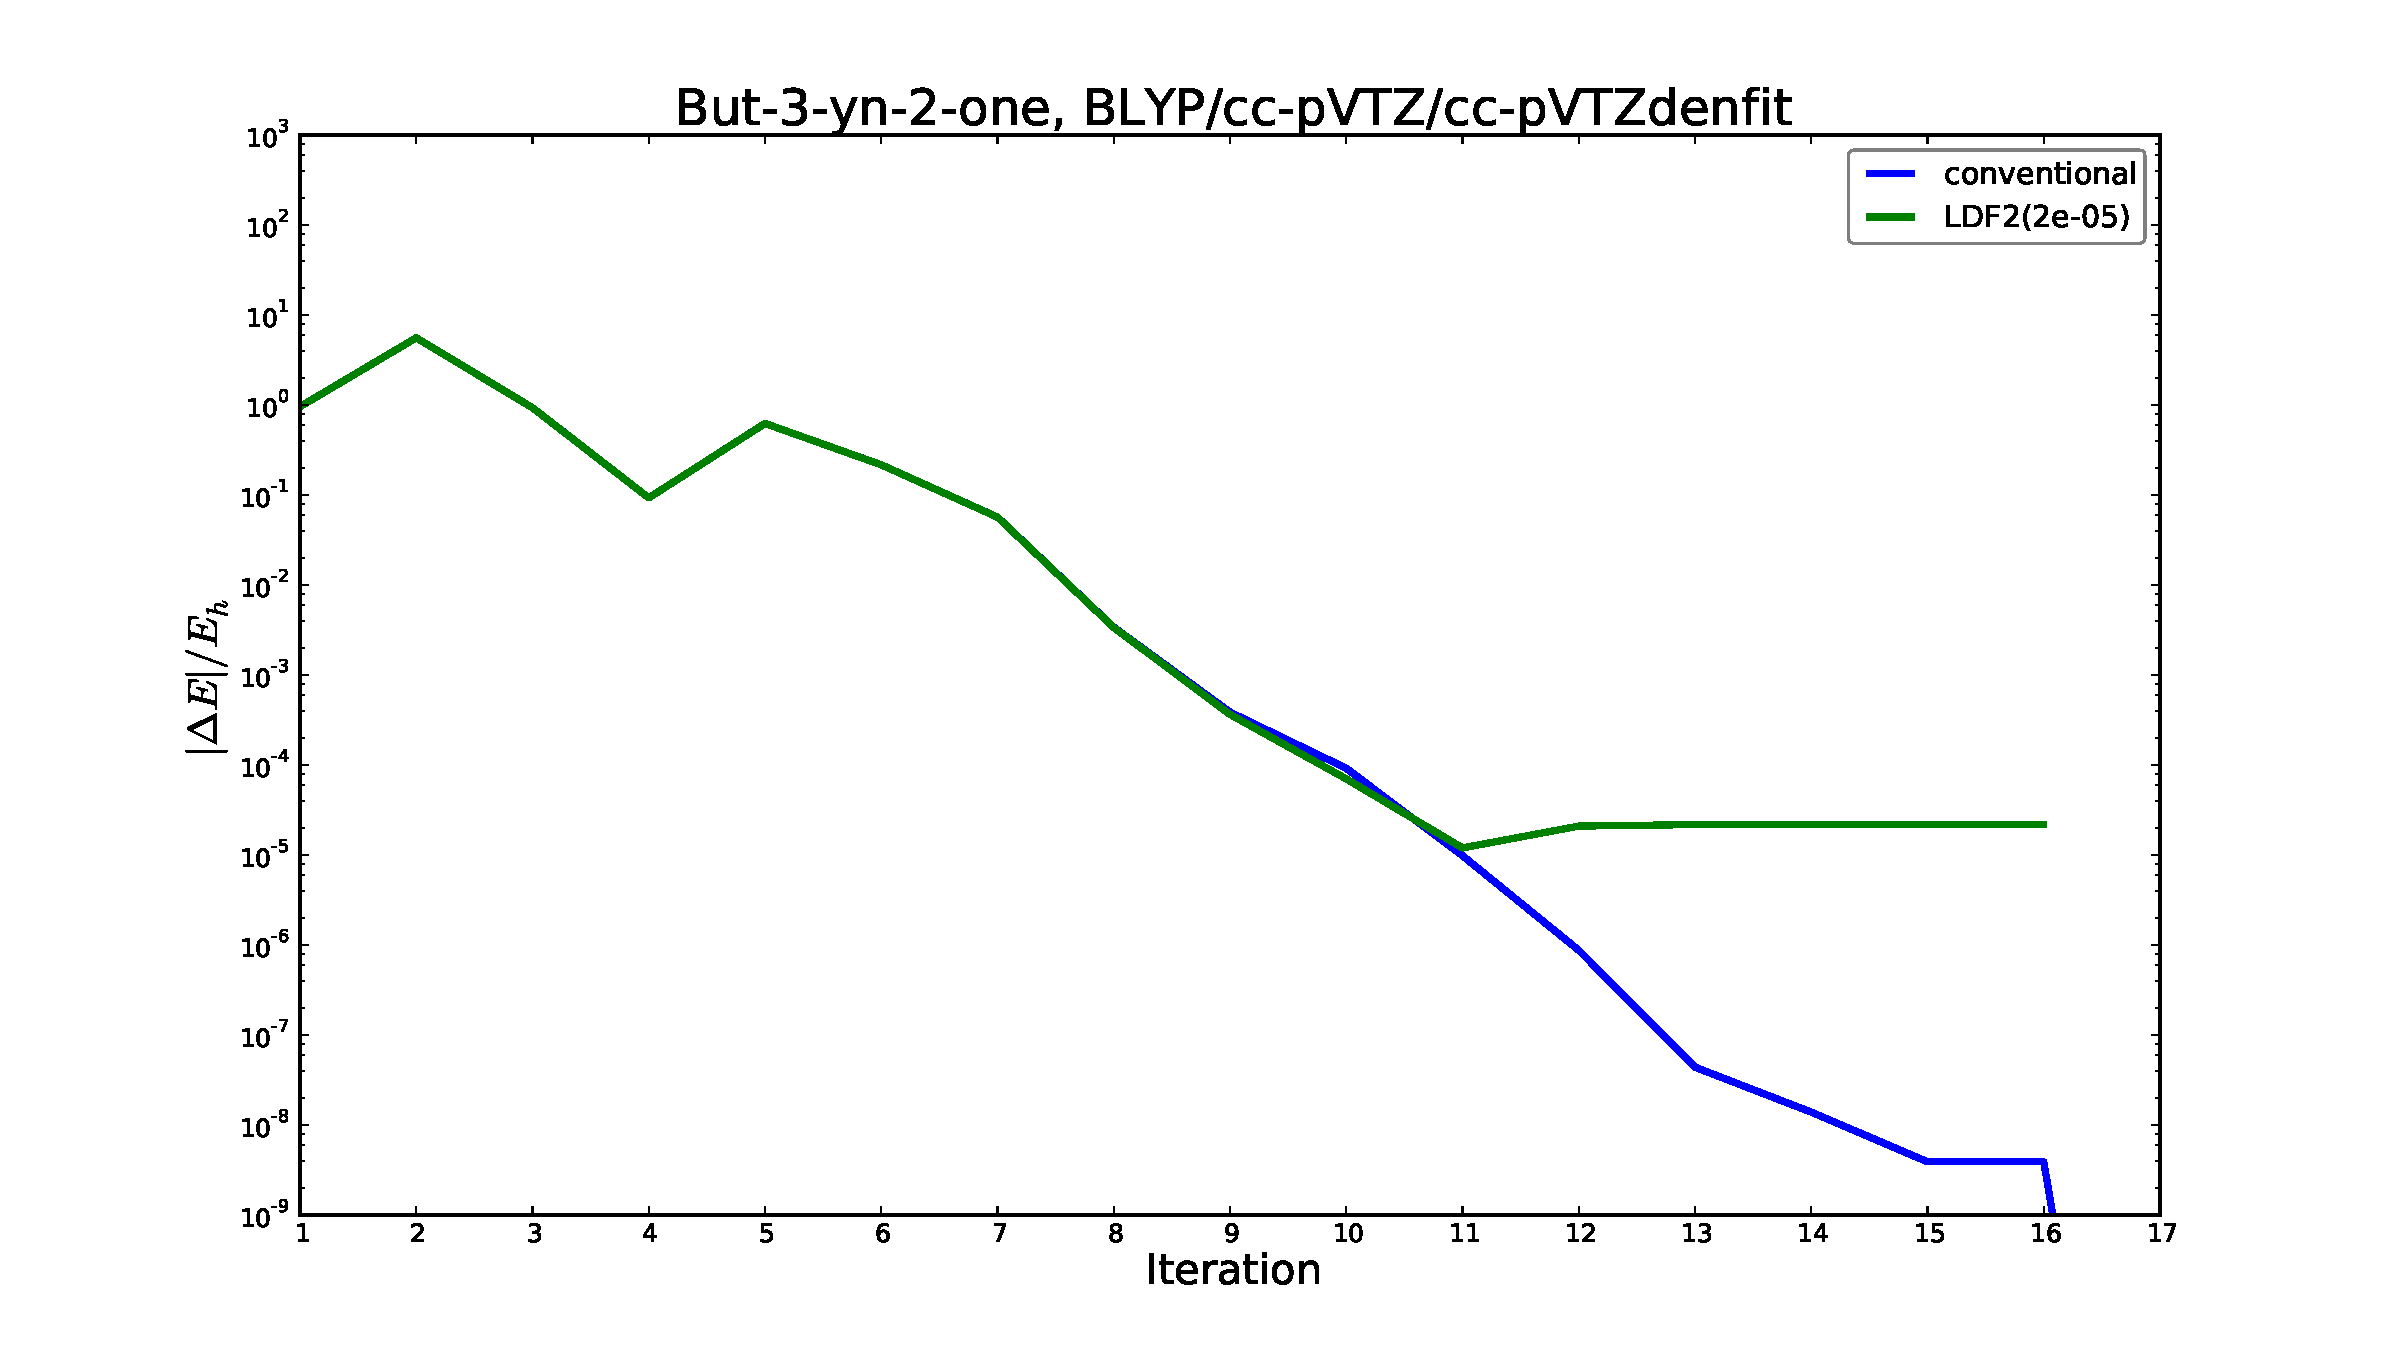
\includegraphics{Figures/conventional_ldf2_5_t2.pdf}
            }
        \end{figure}
    \end{center}
\end{frame}

\begin{frame}
   \frametitle{BLYP cc-pVTZ/cc-pVTZdenfit SCF iterations}
   \tiny{Development version of Molcas, www.molcas.org}
    \begin{center}
        \begin{figure}
            \scalebox{0.3}{
                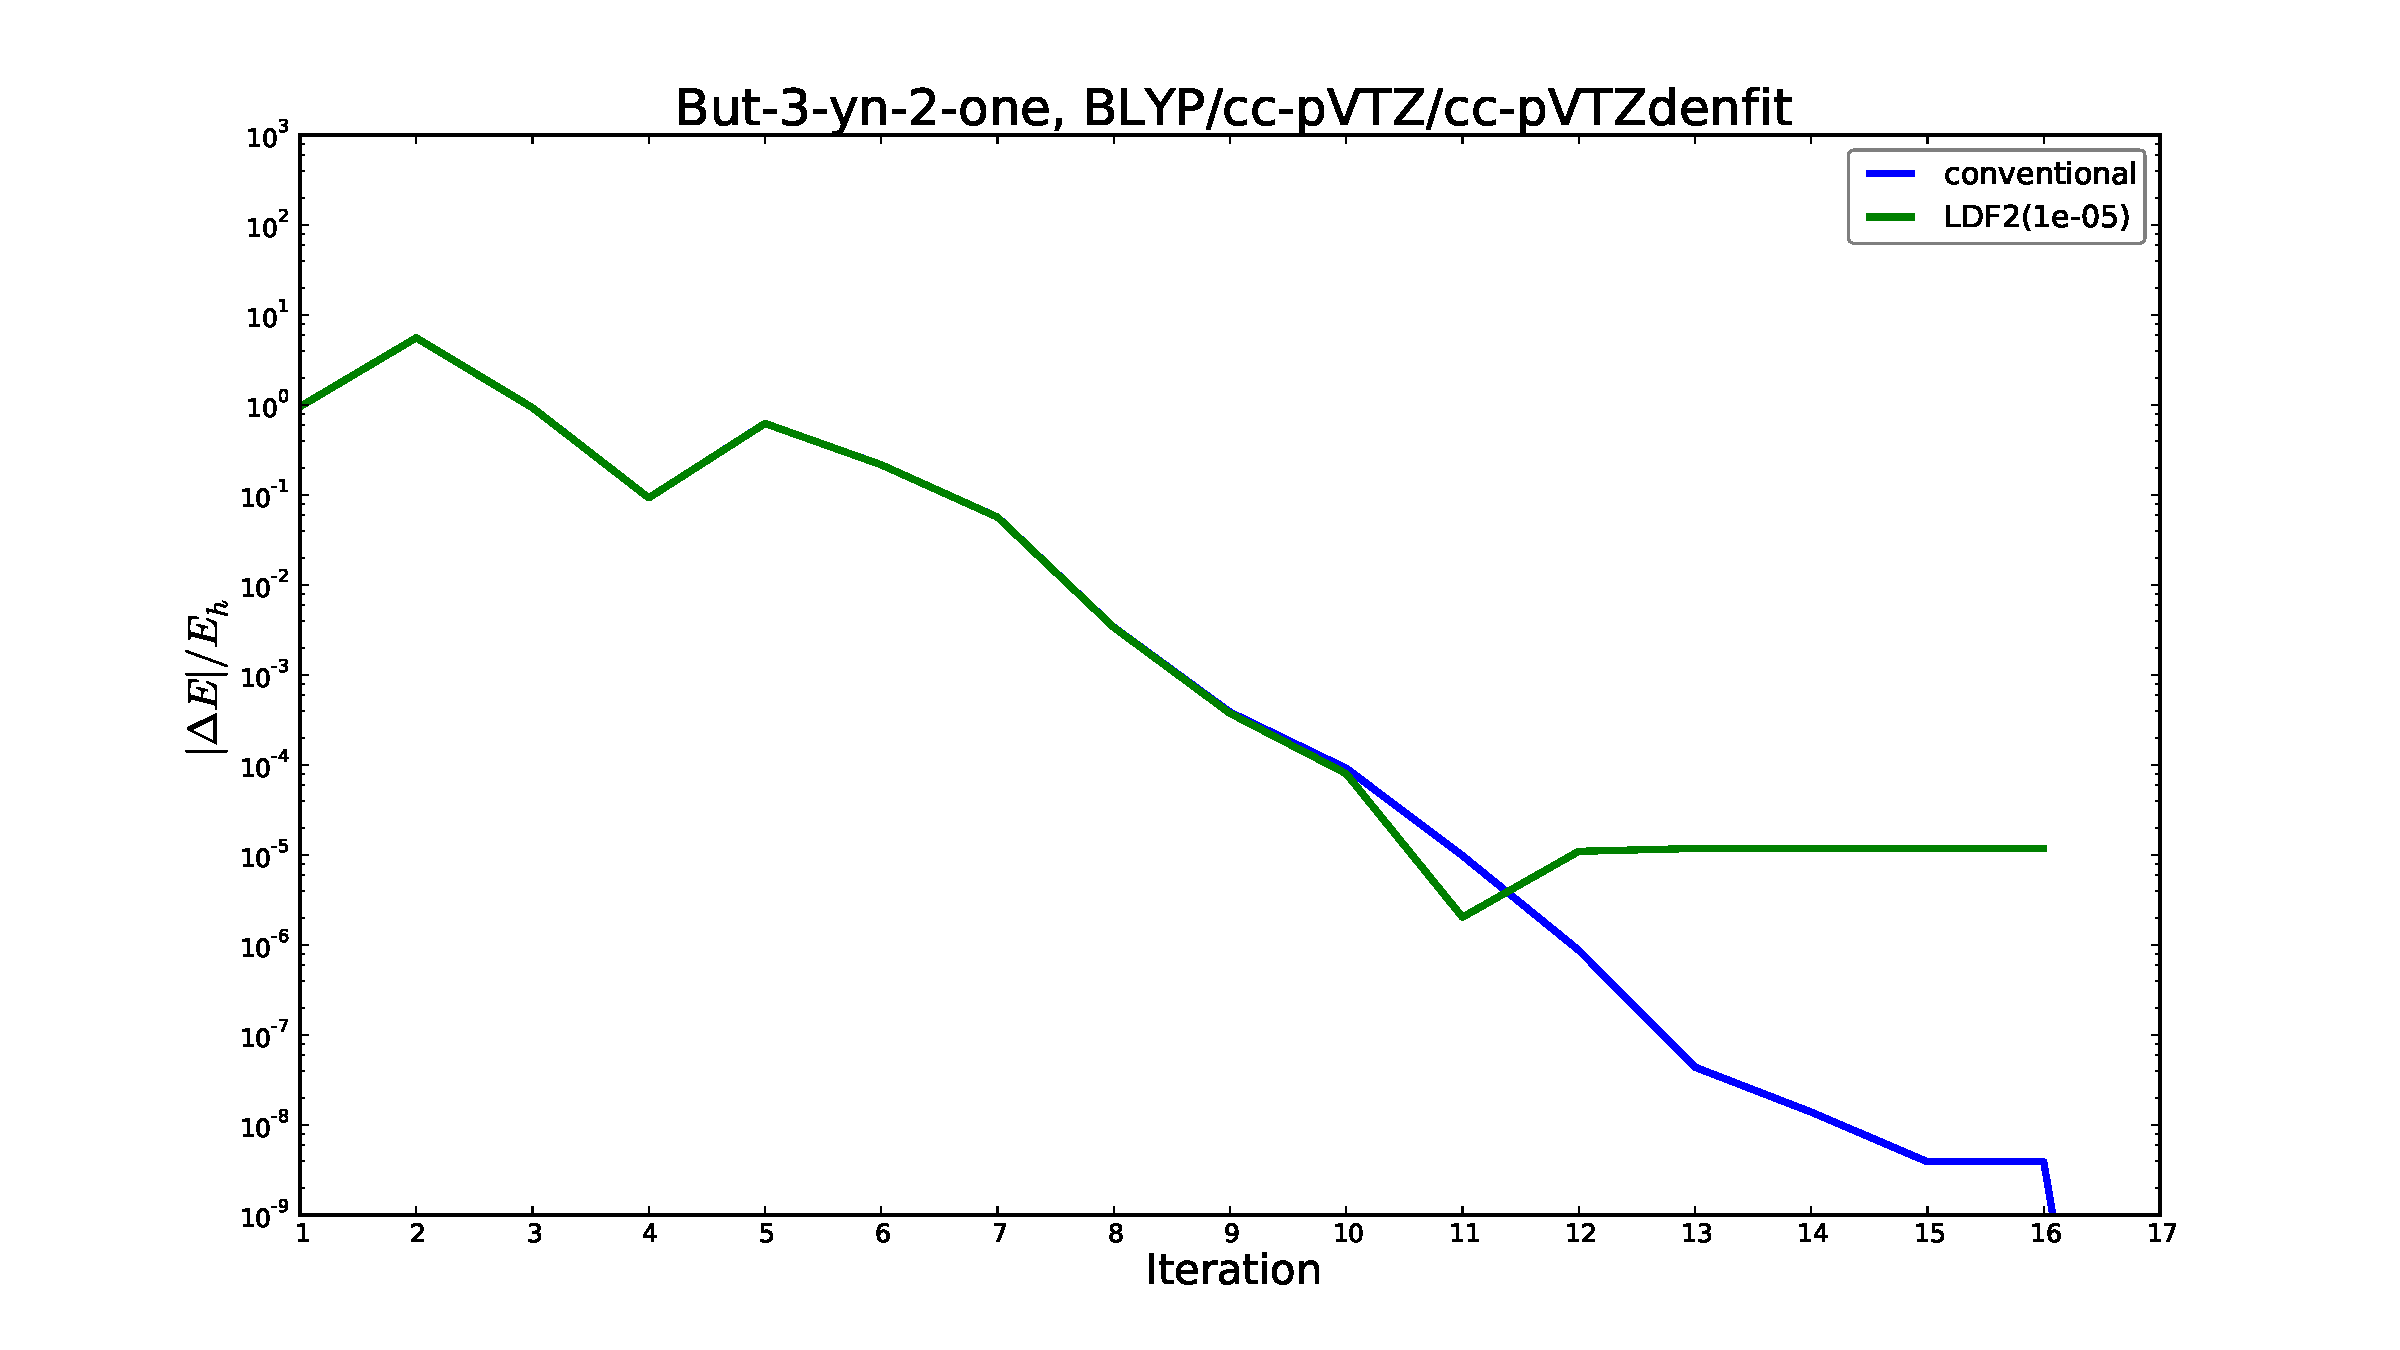
\includegraphics{Figures/conventional_ldf2_5.pdf}
            }
        \end{figure}
    \end{center}
\end{frame}

\begin{frame}
   \frametitle{BLYP cc-pVTZ/cc-pVTZdenfit SCF iterations}
   \tiny{Development version of Molcas, www.molcas.org}
    \begin{center}
        \begin{figure}
            \scalebox{0.3}{
                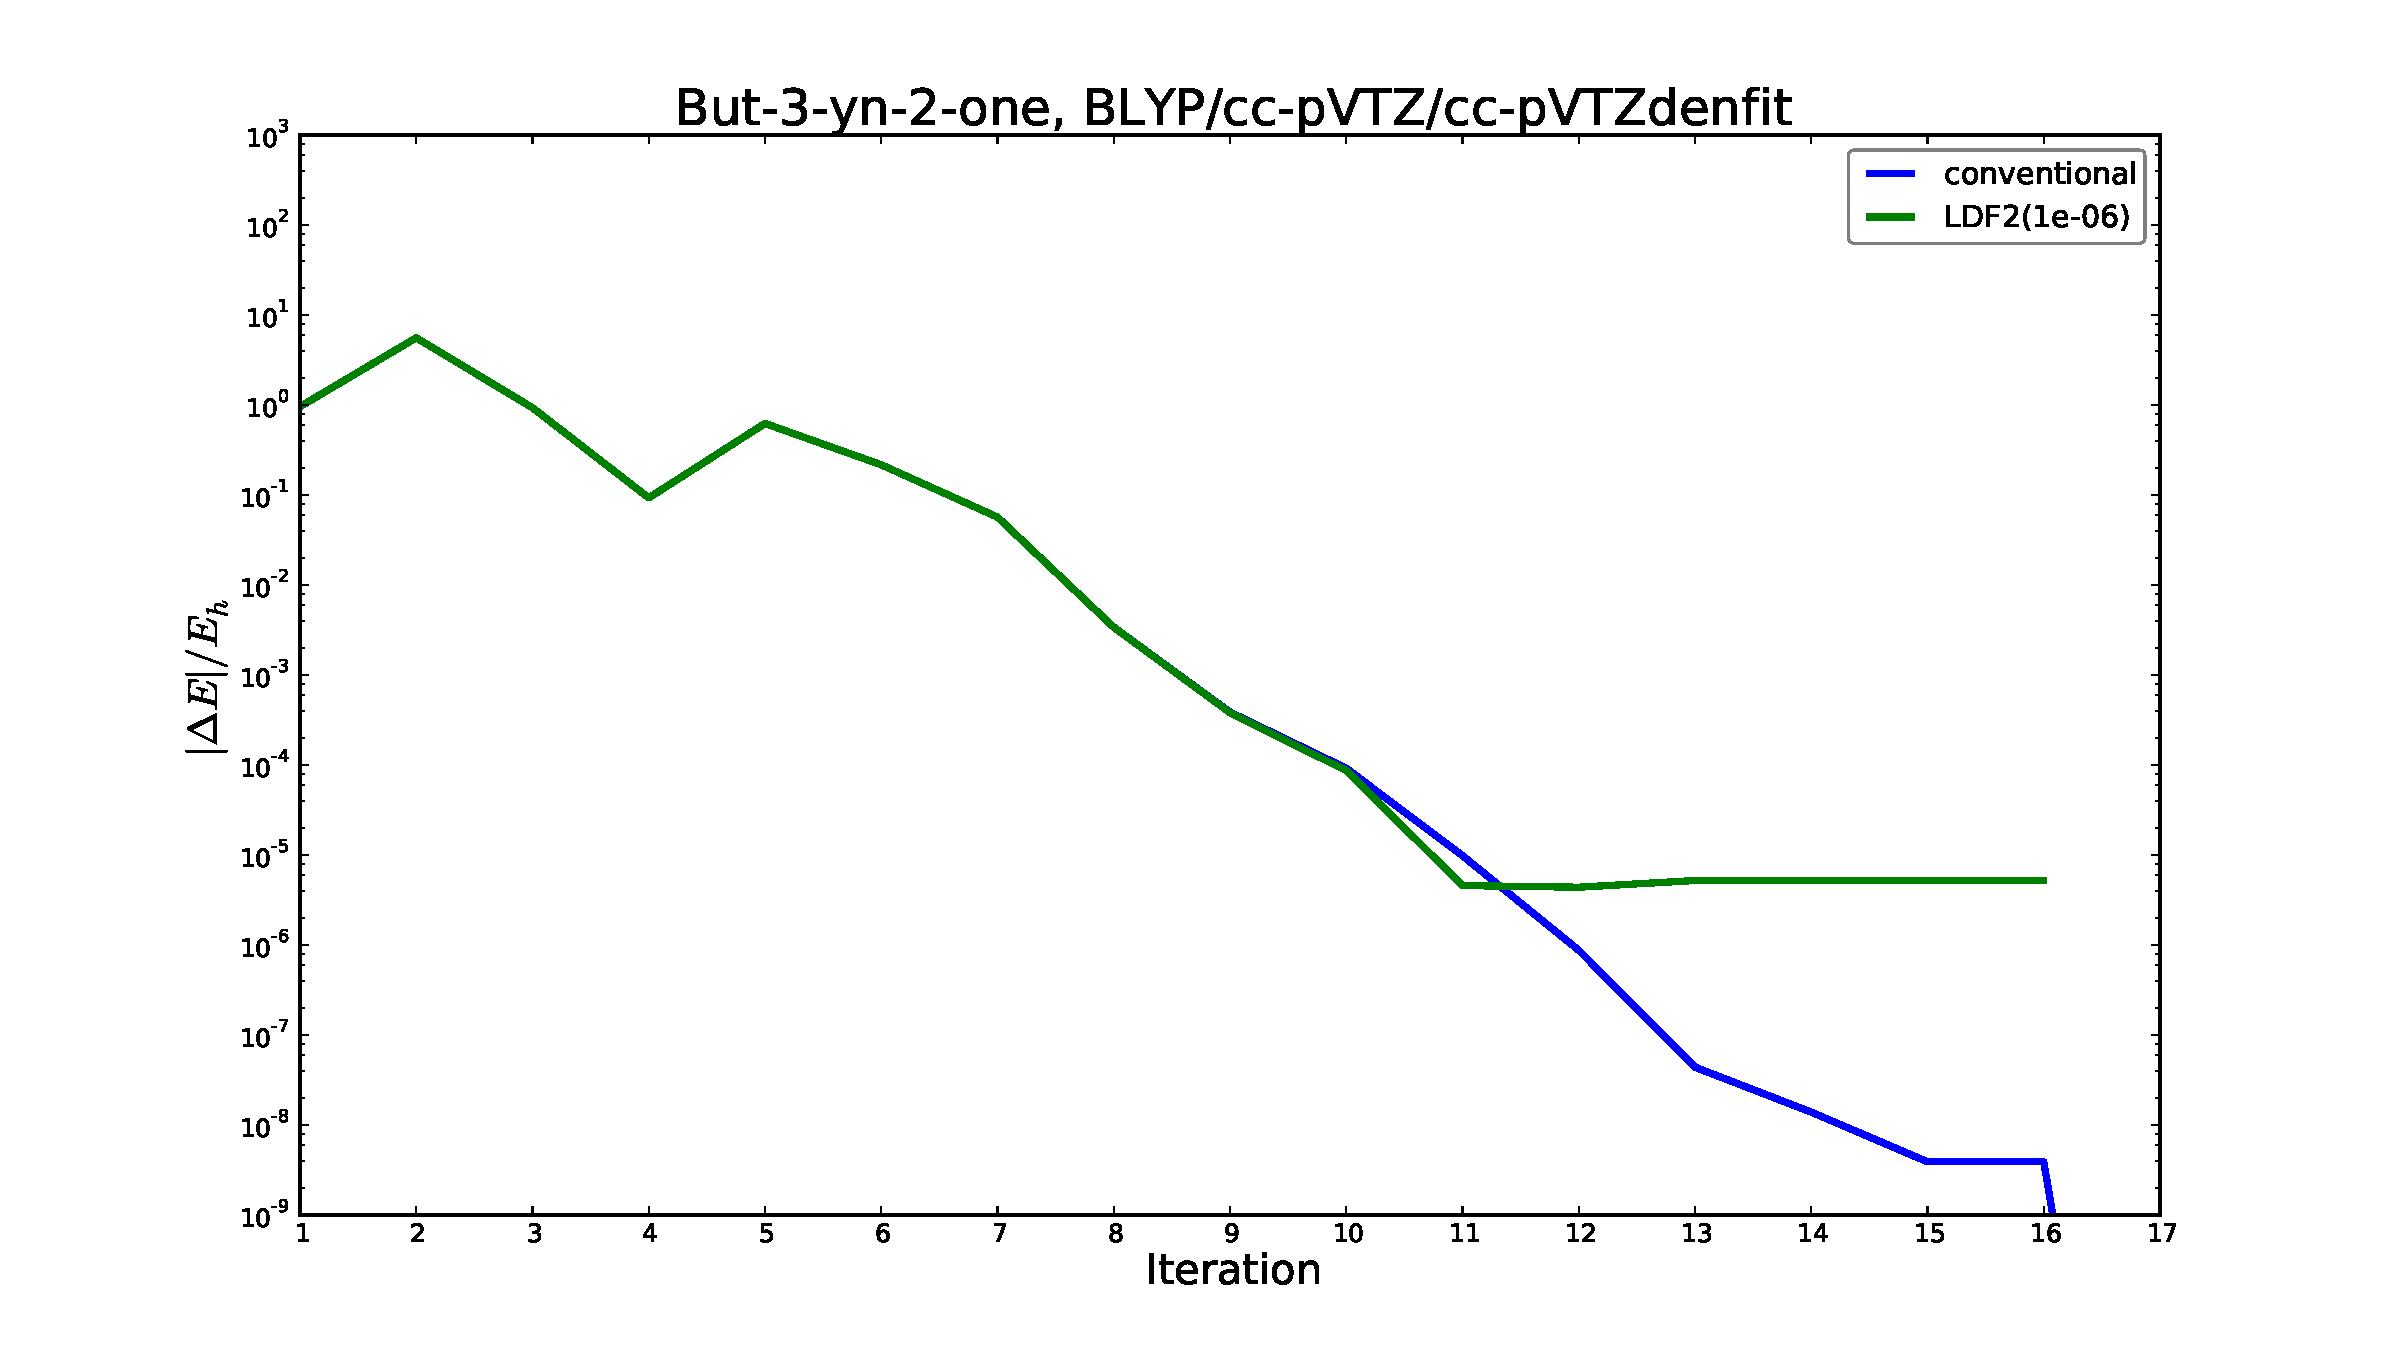
\includegraphics{Figures/conventional_ldf2_6.pdf}
            }
        \end{figure}
    \end{center}
\end{frame}

\begin{frame}
   \frametitle{BLYP cc-pVTZ/cc-pVTZdenfit SCF iterations}
   \tiny{Development version of Molcas, www.molcas.org}
    \begin{center}
        \begin{figure}
            \scalebox{0.3}{
                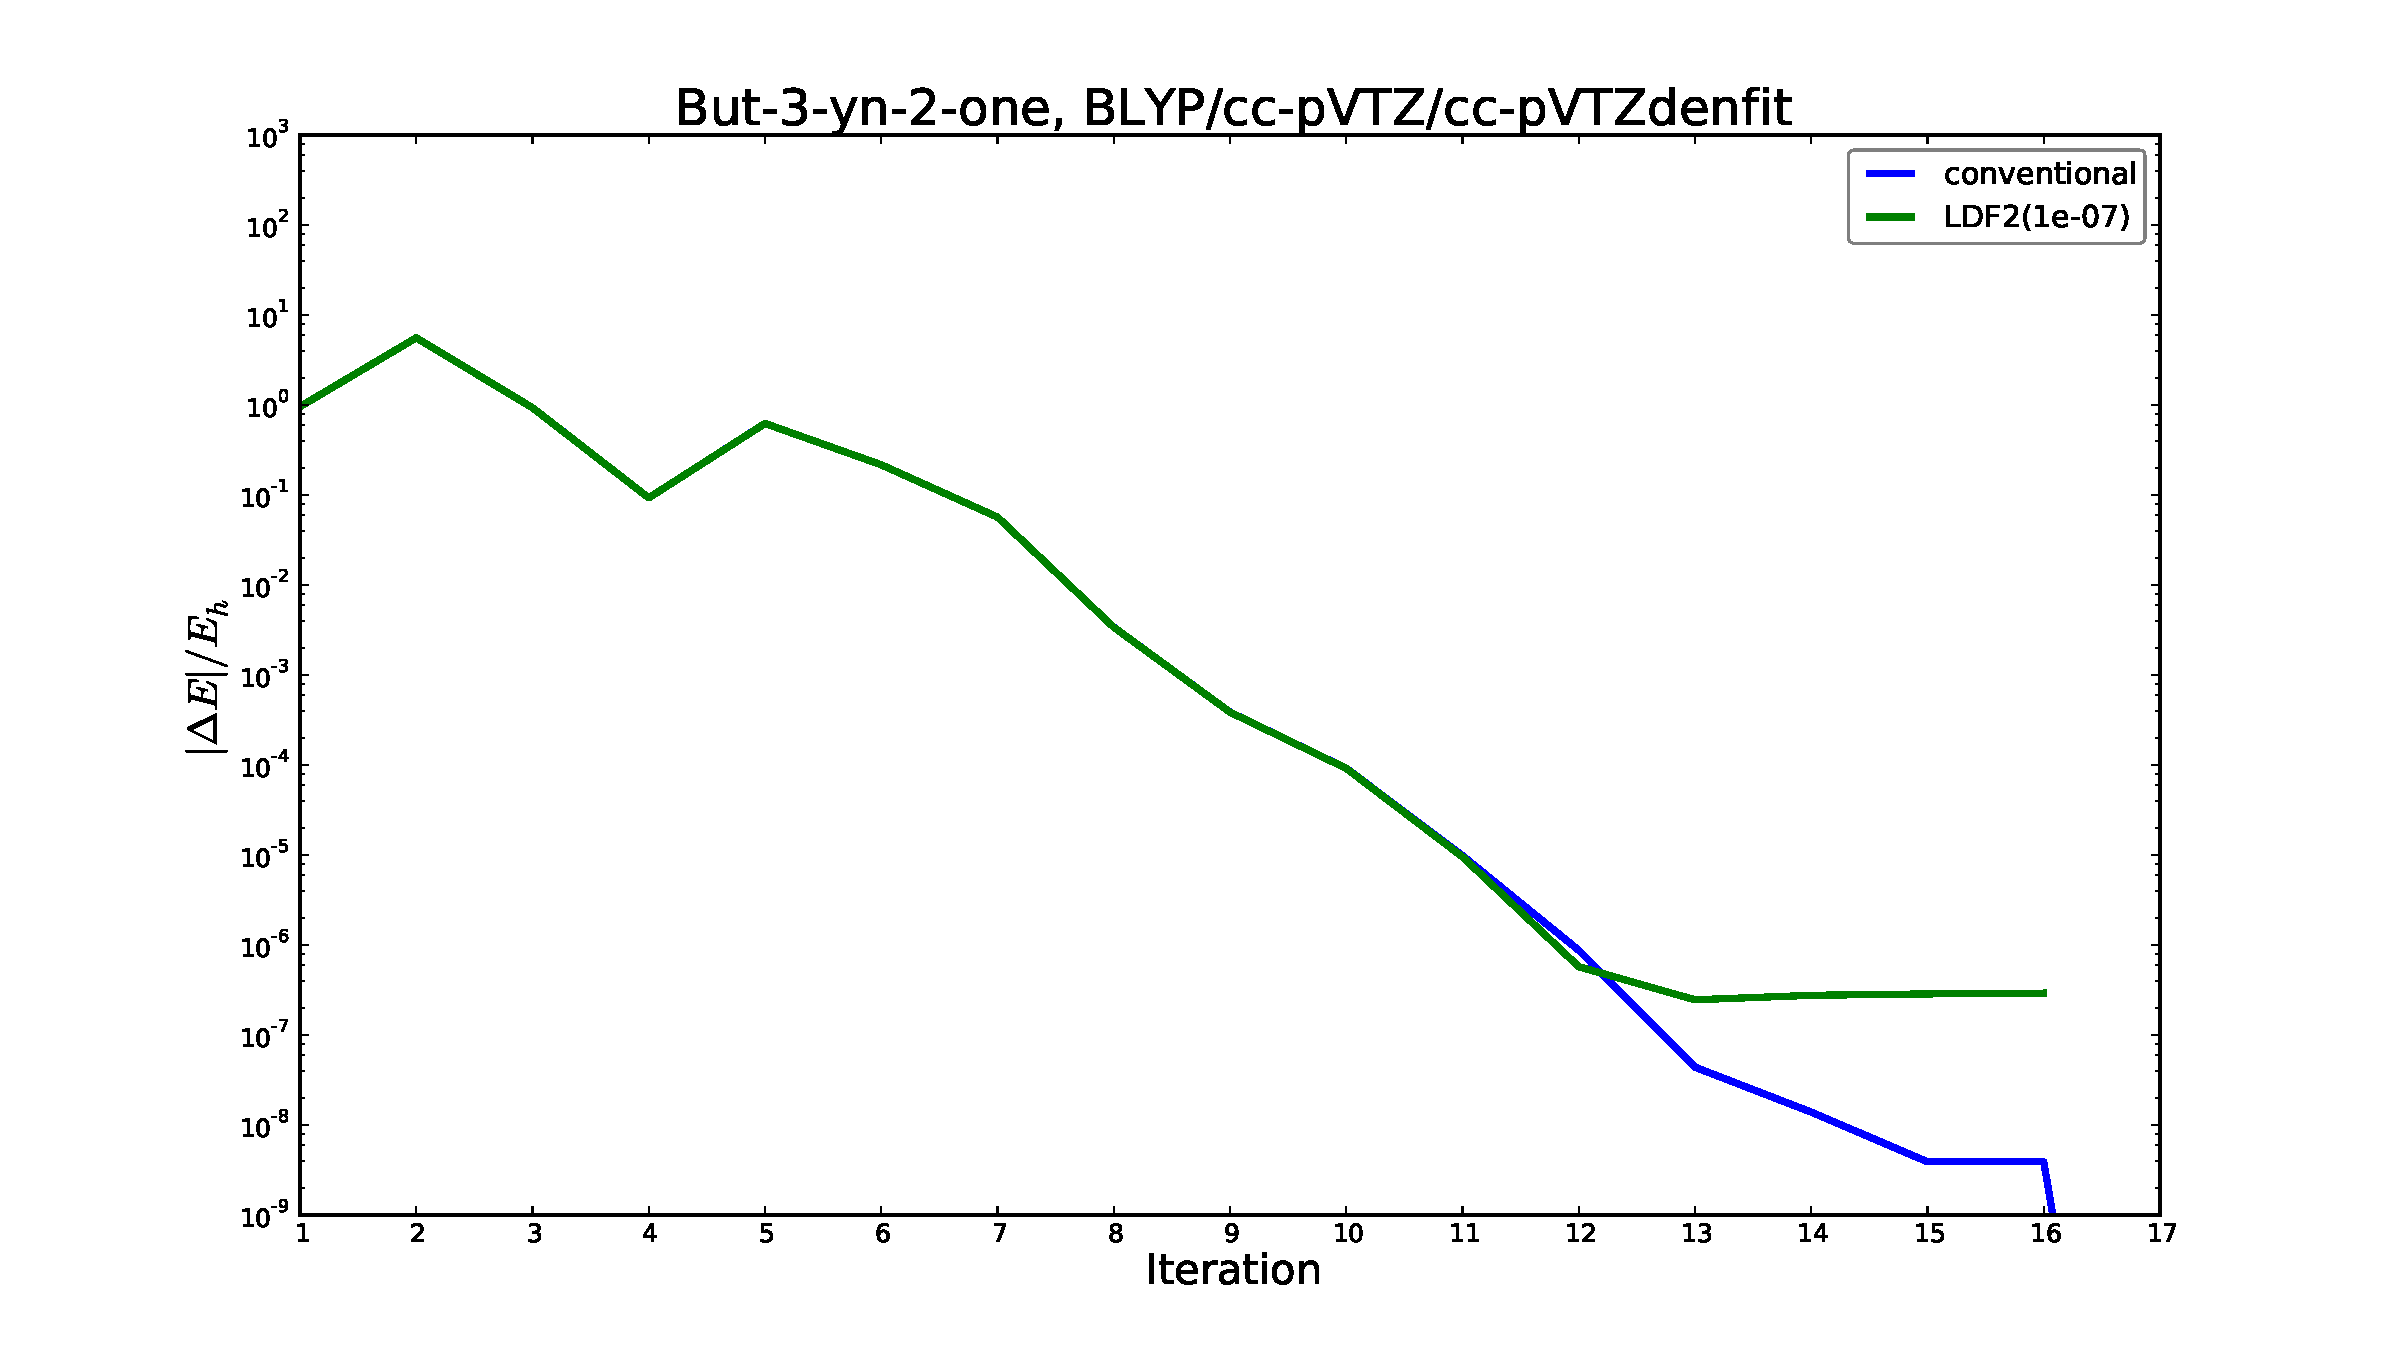
\includegraphics{Figures/conventional_ldf2_7.pdf}
            }
        \end{figure}
    \end{center}
\end{frame}

\begin{frame}
   \frametitle{BLYP cc-pVTZ/cc-pVTZdenfit SCF iterations}
   \tiny{Development version of Molcas, www.molcas.org}
    \begin{center}
        \begin{figure}
            \scalebox{0.3}{
                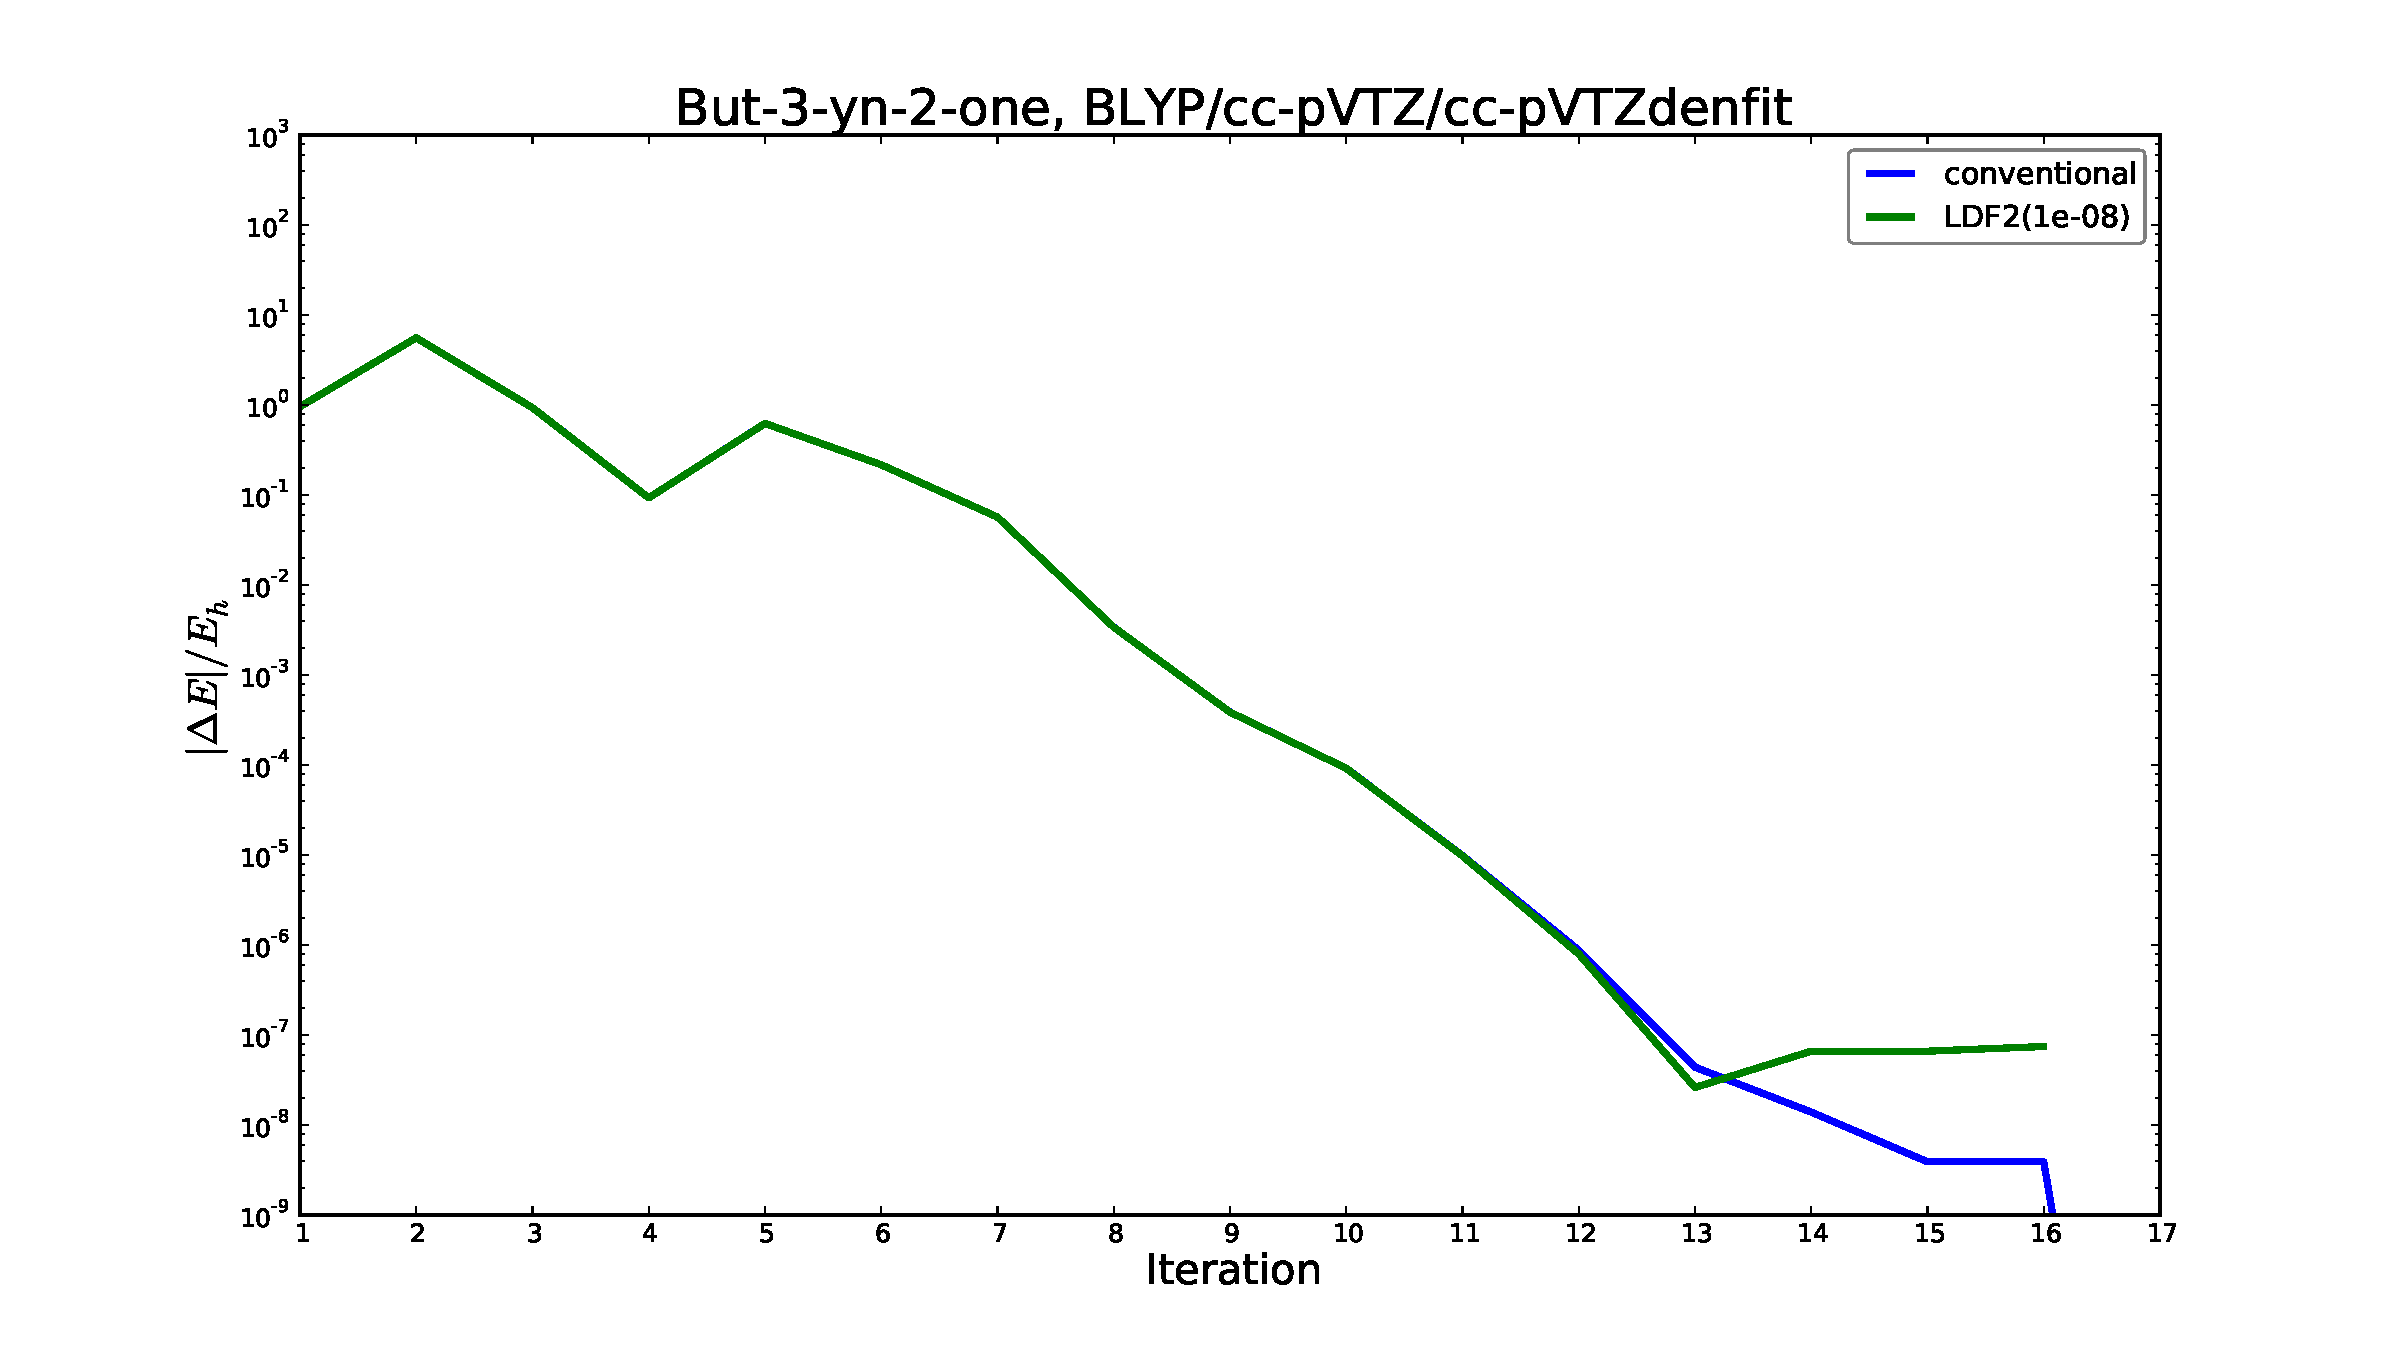
\includegraphics{Figures/conventional_ldf2_8.pdf}
            }
        \end{figure}
    \end{center}
\end{frame}

\begin{frame}
   \frametitle{BLYP cc-pVTZ/cc-pVTZdenfit SCF iterations}
   \tiny{Development version of Molcas, www.molcas.org}
    \begin{center}
        \begin{figure}
            \scalebox{0.3}{
                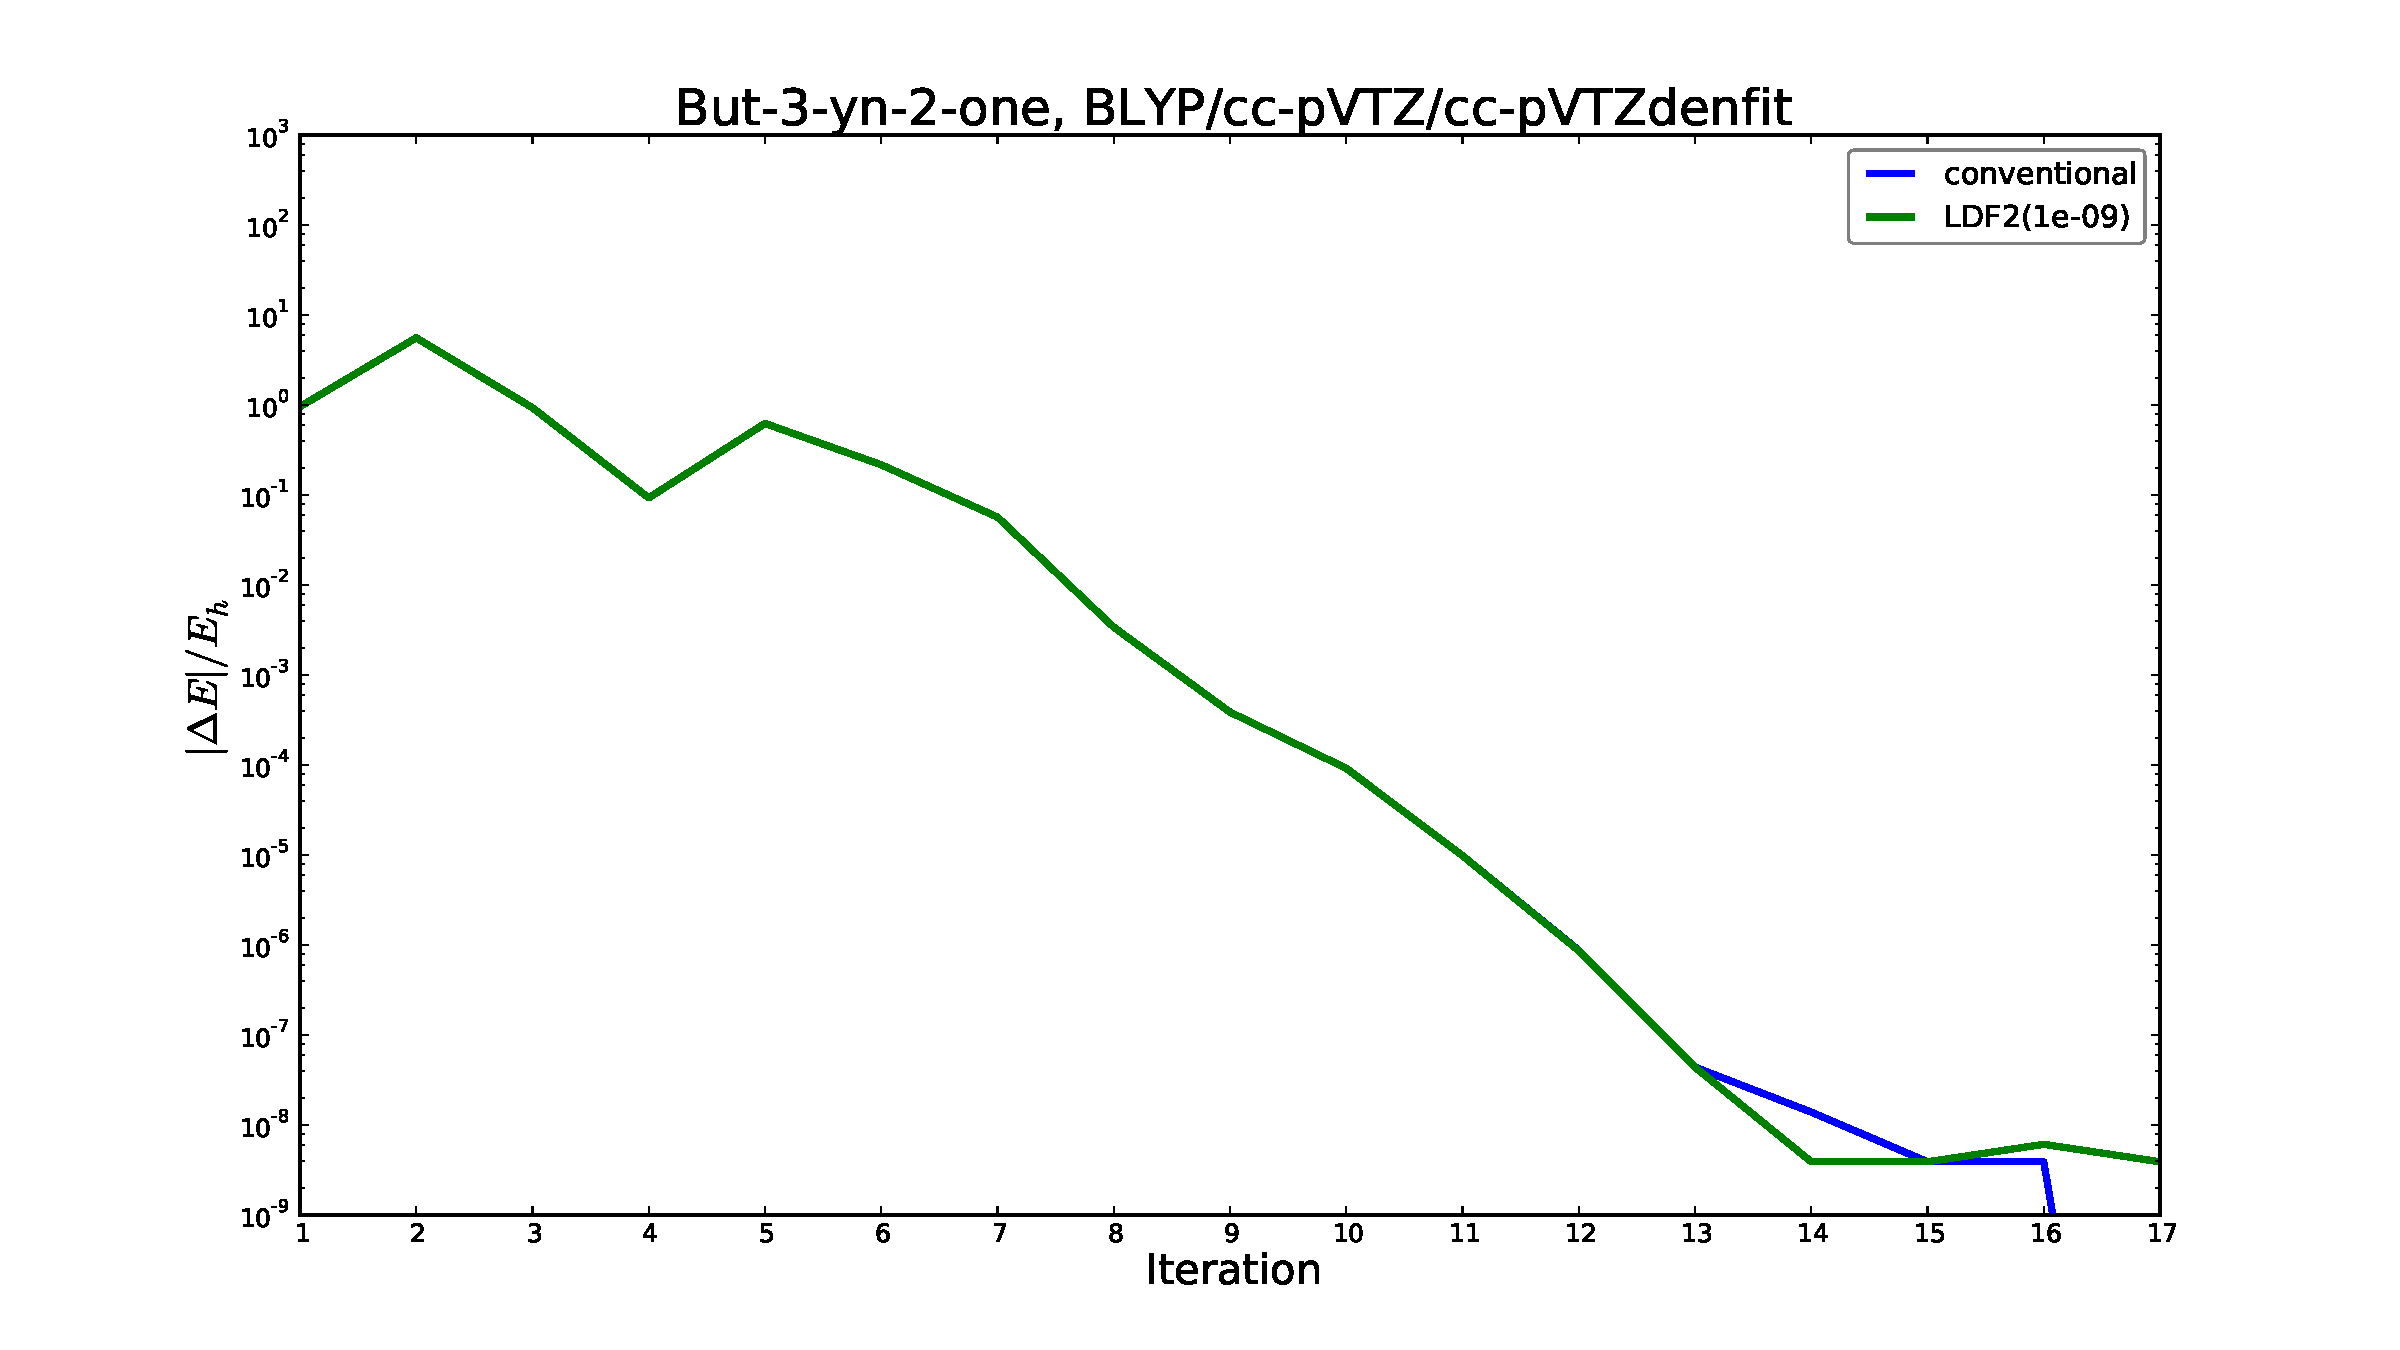
\includegraphics{Figures/conventional_ldf2_9.pdf}
            }
        \end{figure}
    \end{center}
\end{frame}

\begin{frame}
   \frametitle{BLYP cc-pVTZ/cc-pVTZdenfit SCF iterations}
   \tiny{Development version of Molcas, www.molcas.org}
    \begin{center}
        \begin{figure}
            \scalebox{0.3}{
                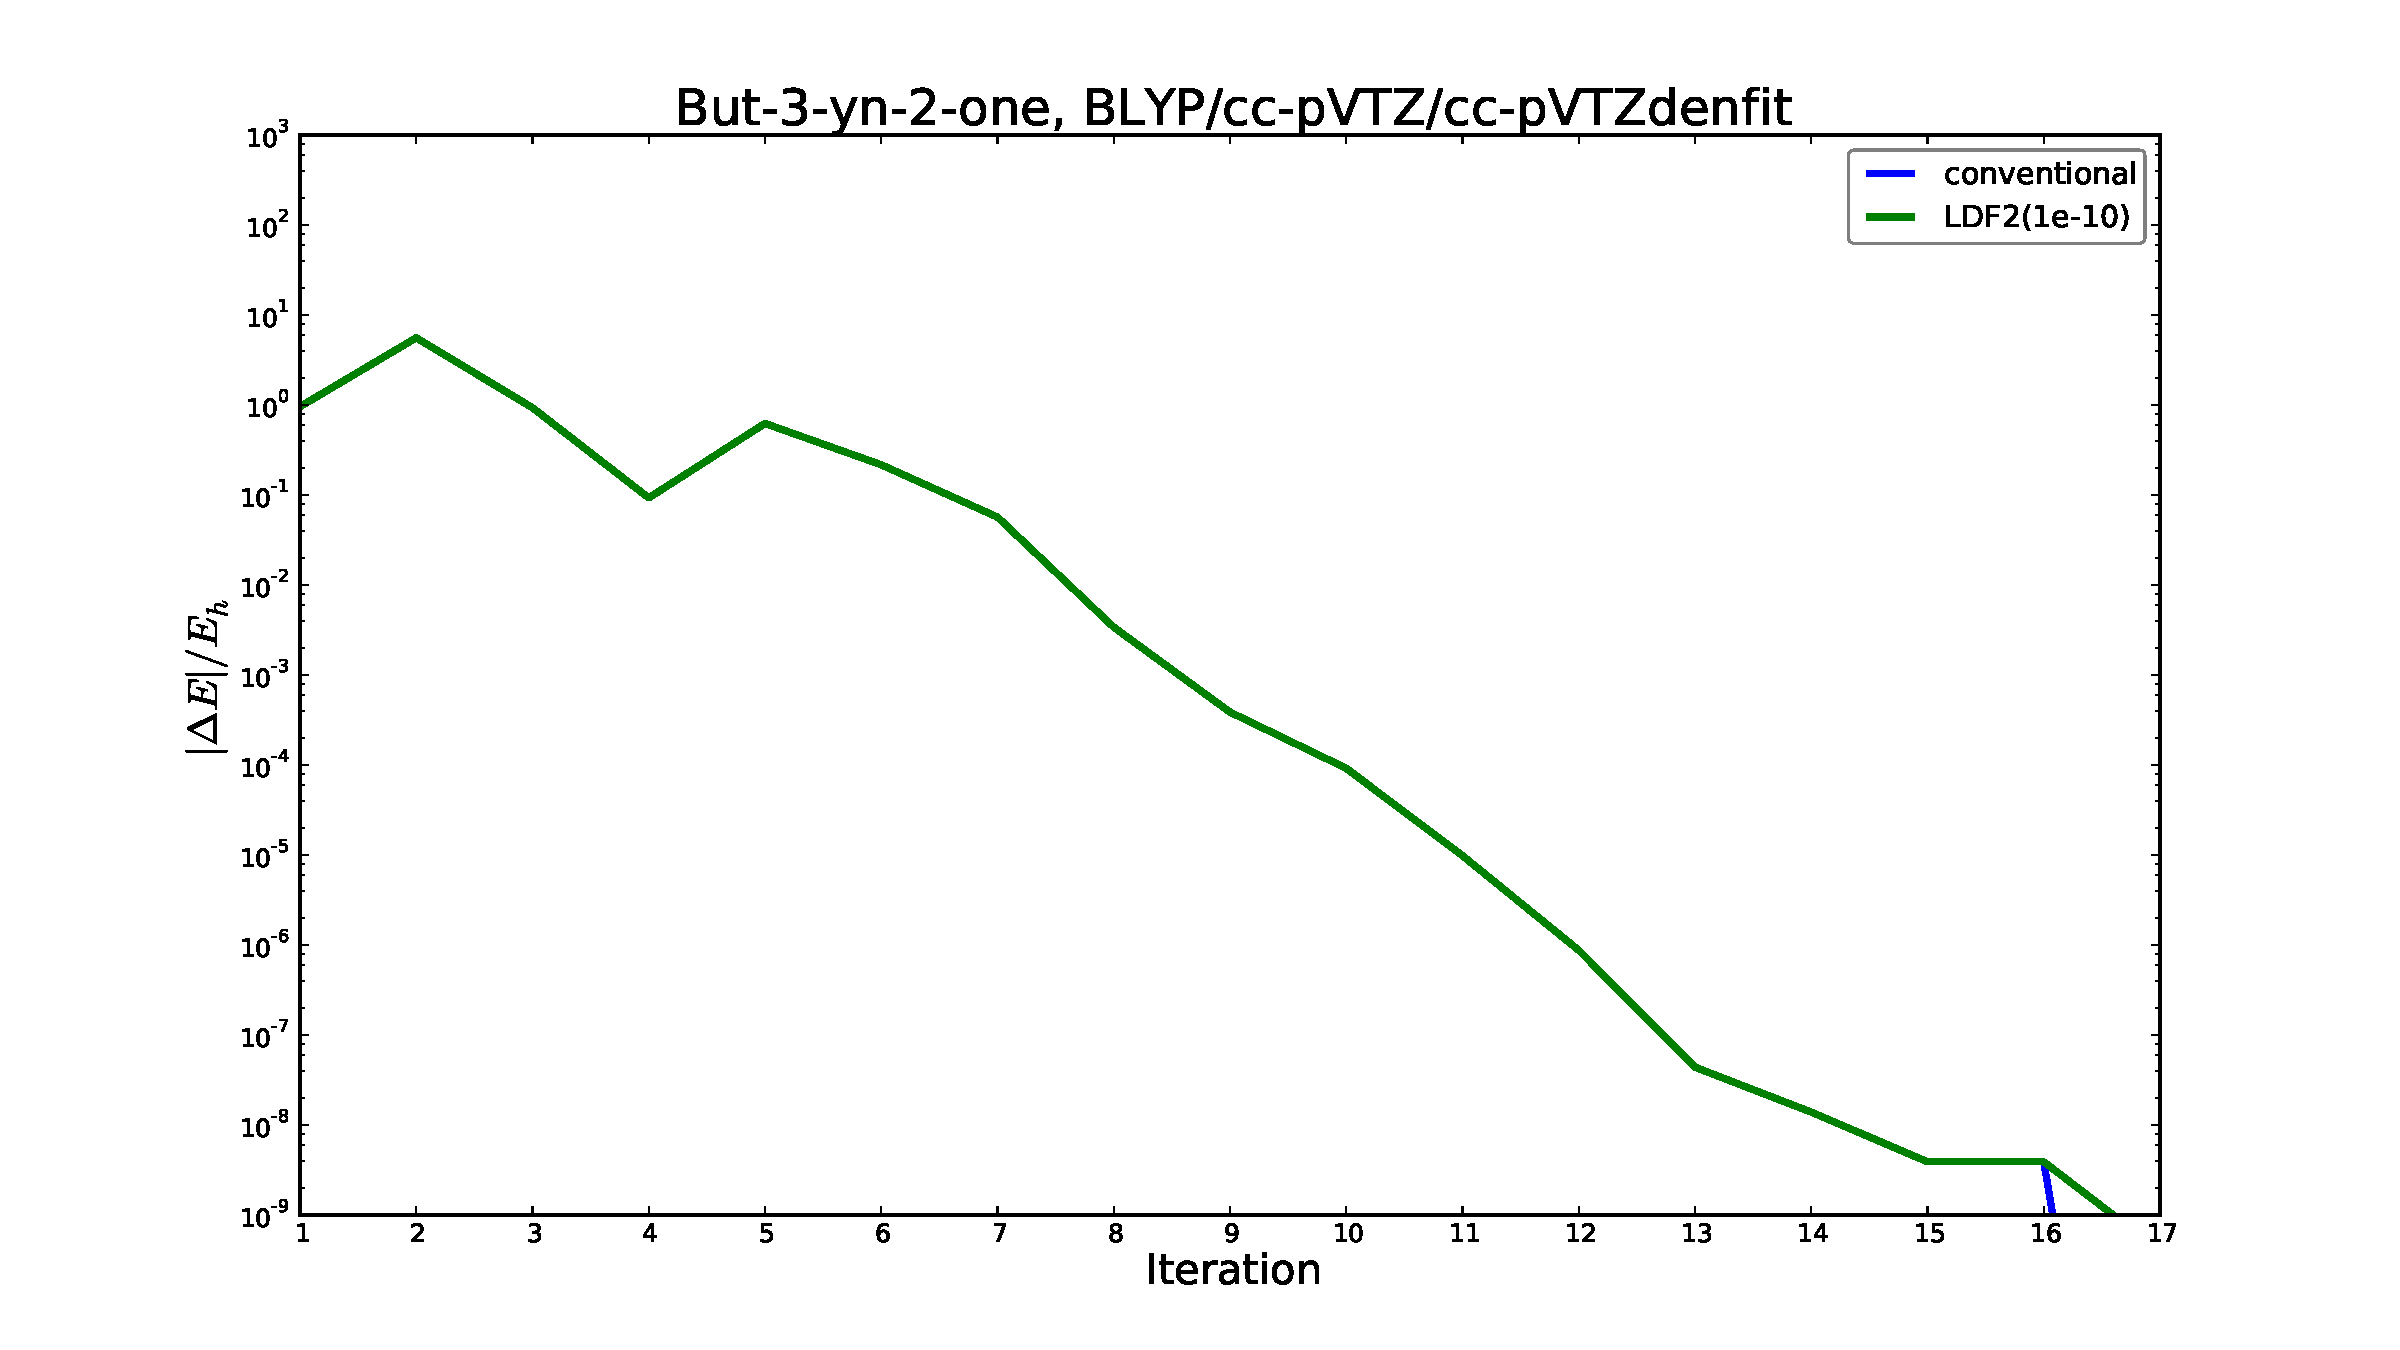
\includegraphics{Figures/conventional_ldf2_10.pdf}
            }
        \end{figure}
    \end{center}
\end{frame}


%% \section{But-3-yn-2-one: negative ERI eigenvalues}
%% \begin{frame}
%%    \frametitle{BLYP cc-pVTZ/cc-pVTZdenfit negative ERI eigenvalues}
%%    \tiny{Development version of Molcas, www.molcas.org}
%%     \begin{center}
%%         \begin{figure}
%%             \scalebox{0.3}{
%%                 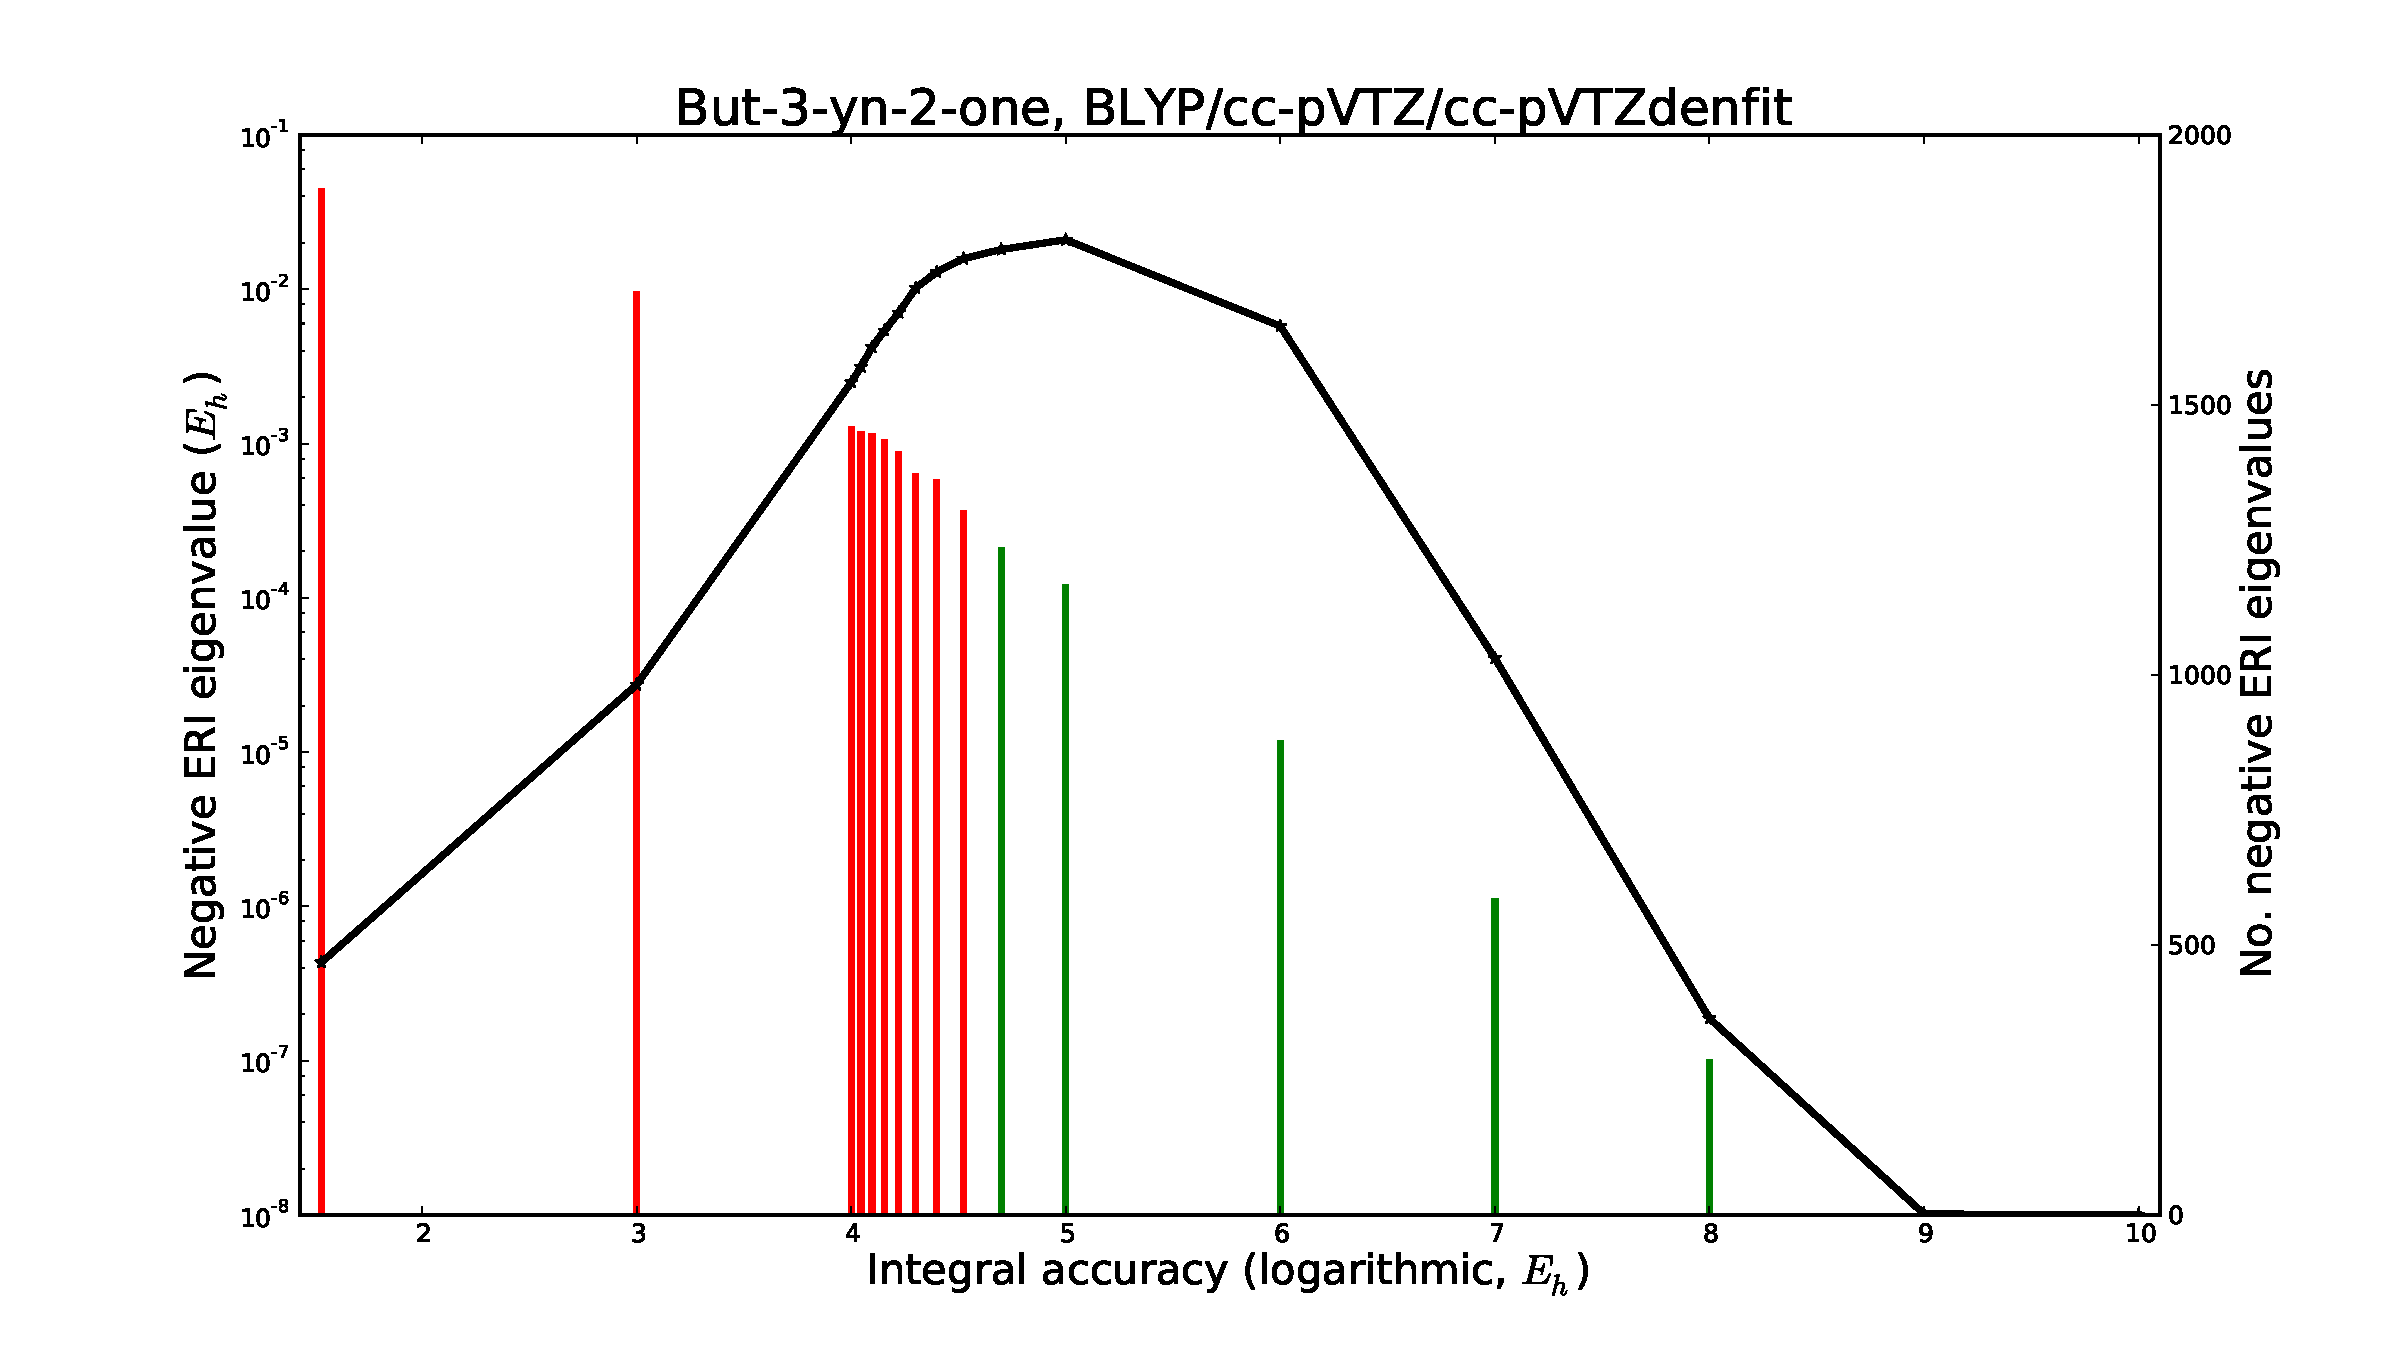
\includegraphics{Figures/negEig.pdf}
%%             }
%%         \end{figure}
%%     \end{center}
%% \end{frame}

\section{Conclusions}

\begin{frame}
   \frametitle{Conclusions}
   \begin{itemize}
      \item PARI \st{is} was promising
      \item When it fails, it fails spectacularly!
      \item Reason: small attractive forces between the electrons.
      \item Present in all local domain fitting schemes (using robust or similar integral representations).
      \item Only known solution: locally complete fitting basis.
      \item We use two-center functions selected by Cholesky decomposition of the fitting error matrix for each atom pair.
      \item Problems:
            \begin{itemize}
              \footnotesize
                 \item Slows down the calculation, even compared to conventional (up to a factor of 2 slow-down has been  observed for smallish molecules).
                 \item Fitting basis becomes geometry-dependent $\Longrightarrow$ discontinuities.
            \end{itemize}
   \end{itemize}
\end{frame}

\section{Acknowledgments}
\begin{frame}
   \begin{itemize}
        \item Organizers for the invitation
        \item Collaborators
          \begin{itemize}
          \item Prof. Trygve Helgaker
          \item Dr. Simen Reine
          \item Dr. Thomas Bondo Pedersen
          \item Dr. Thomas Kj{\ae}rgaard
          \end{itemize}
          
        \item Funding
          \begin{center}
            
\includegraphics[height=1.5cm]{uio.pdf}\hspace{1cm}
            
\includegraphics[height=1.5cm]{sff.pdf}\hspace{1cm}
            
\includegraphics[width=3cm]{notur_large.png}\hspace{1cm}
          \end{center}
   \end{itemize}
\end{frame}


